\documentclass[11pt,a4paper]{article}

%================================================
% Packages and formatting
%================================================

%================================================
% Page layout
%================================================

\usepackage[
    a4paper,
    margin=2.5cm
]{geometry}

%================================================
% Mathematics
%================================================

\usepackage{amsmath}
\usepackage{amssymb}
\usepackage{amsfonts}
\usepackage{bm}

%================================================
% Figures and tables
%================================================

\usepackage{graphicx}
\usepackage{float}
\usepackage{subcaption}
\usepackage{booktabs}
\usepackage{caption}
\usepackage{tabularx}

%================================================
% Fonts and typography
%================================================

\usepackage[T1]{fontenc}
\usepackage{lmodern}

\usepackage{setspace}
\setstretch{1.1}

\setlength{\parindent}{0pt}
\setlength{\parskip}{0.6em}

%================================================
% Section formatting
%================================================

\usepackage{titlesec}

\titleformat{\section}
{\Large\bfseries}
{\thesection.}
{0.6em}
{}

\titleformat{\subsection}
{\large\bfseries}
{\thesubsection}
{0.6em}
{}

\titlespacing*{\section}
{0pt}{18pt}{10pt}

\titlespacing*{\subsection}
{0pt}{12pt}{6pt}

%================================================
% Hyperlinks
%================================================

\usepackage[
colorlinks=true,
linkcolor=blue,
citecolor=blue,
urlcolor=blue
]{hyperref}

%================================================
% Header and footer
%================================================

\usepackage{fancyhdr}

\pagestyle{fancy}

\fancyhf{}

\fancyhead[L]{CFD Portfolio}
\fancyhead[R]{Project 01}

\fancyfoot[C]{\thepage}

\renewcommand{\headrulewidth}{0.4pt}

\setlength{\headheight}{25pt}
\setlength{\headsep}{25pt}

%================================================
% Lists
%================================================

\usepackage{enumitem}

\setlist{
itemsep=3pt,
topsep=5pt
}

%================================================
% Figure captions
%================================================

\captionsetup{
font=small,
labelfont=bf
}
\renewcommand{\arraystretch}{0.9}
\setlength{\abovecaptionskip}{4pt}
\setlength{\belowcaptionskip}{4pt}
\setlength{\intextsep}{8pt}

%================================================
% Table spacing
%================================================

\renewcommand{\arraystretch}{1.25}

%================================================
% Document information
%================================================

\title{
    \Huge\textbf{Parameterized Two-Dimensional
    Steady-State Energy Equation}\\[0.4cm]
    \Large
    Full-Order Numerical Modeling, Discrete
    Galerkin--POD Reduction, and
    Error-Guided Snapshot Enrichment
}

\author{
    \Large Arian Shahnoori
}

\date{\today}

%================================================
\begin{document}
%================================================

%------------------------------------------------
% Title and abstract
%------------------------------------------------

\pagenumbering{gobble}

\maketitle

\begin{abstract}
A numerical framework is developed for the solution and
reduced-order modeling of a parameterized two-dimensional
steady-state energy equation with prescribed velocity and
viscous dissipation. The full-order model employs a
cell-centered second-order spatial discretization with
ghost-cell boundary treatment and an iterative procedure
for obtaining steady-state solutions. A proper orthogonal
decomposition (POD) basis is constructed from parameterized
full-order solutions, and a reduced-order model is developed
through Galerkin projection of the discrete spatial operators.
The accuracy of the reduced-order model is evaluated for
different numbers of retained modes using independent
parameter samples. An error-guided snapshot enrichment
strategy is subsequently investigated by selecting additional
full-order solutions from regions associated with relatively
large approximation errors. The original and augmented POD
bases are compared using a common independent test dataset
to assess the effect of enrichment on reduced-order accuracy
across the parameter domain.
\end{abstract}

\vspace{0.4cm}

%------------------------------------------------
% Problem overview
%------------------------------------------------

\begin{center}
    \textbf{Study Overview}

    \vspace{0.15cm}

    {\small
    \renewcommand{\arraystretch}{1.15}
    \setlength{\tabcolsep}{5pt}

    \begin{tabular}{@{}p{0.27\textwidth}p{0.68\textwidth}@{}}
        \toprule
        \textbf{Problem} &
        Parameterized two-dimensional steady-state energy equation \\

        \textbf{Governing physics} &
        Convection, thermal diffusion, and viscous dissipation \\

        \textbf{Computational domain} &
        Rectangular channel ($L_x\times L_y=5\times1$) \\

        \textbf{Velocity field} &
        Prescribed parabolic profile \\

        \textbf{Spatial discretization} &
        Cell-centered second-order central differences \\

        \textbf{Computational grid} &
        $N_x\times N_y=50\times20$ \\

        \textbf{Boundary treatment} &
        Ghost-cell boundary closures \\

        \textbf{Full-order solver} &
        Backward-Euler pseudo-time marching with sparse LU factorization \\

        \textbf{Reduced-order method} &
        Proper orthogonal decomposition and discrete Galerkin projection \\

        \textbf{Parameter space} &
        $c=1$, $\mu=cPe\in[1,100]$, $Br\in[0.01,2]$ \\

        \textbf{Basis enrichment} &
        Error-guided local snapshot enrichment \\

        \textbf{Evaluation metrics} &
        Relative $L_2$ error, RMSE, and maximum absolute error \\

        \textbf{Programming language} &
        Python \\
        \bottomrule
    \end{tabular}
    }
\end{center}

%================================================
% Contents
%================================================

\clearpage

\pagenumbering{roman}

\tableofcontents

\clearpage

%================================================
% Main report
%================================================

\pagenumbering{arabic}

\section{Introduction}

\subsection{Motivation}

Repeated numerical solutions of parameterized partial differential equations can be computationally expensive, particularly when a large number of parameter combinations must be investigated. Reduced-order modelling offers an alternative by representing the solution in a low-dimensional space.

Proper orthogonal decomposition (POD) extracts dominant spatial modes from full-order solutions, while Galerkin projection transforms the governing equations into a reduced system. However, high POD energy retention does not necessarily guarantee accurate predictions across the entire parameter domain. Therefore, the performance of a reduced-order model must also be assessed at parameter combinations not used during basis construction.

\subsection{Problem Statement and Objectives}

This study develops a discrete Galerkin--POD reduced-order model for a parameterized two-dimensional steady-state energy equation. The main objectives are:

\begin{enumerate}
    \item Develop a full-order numerical model and generate parameterized temperature solutions.
    \item Construct a POD basis using singular value decomposition.
    \item Develop a reduced-order model through discrete Galerkin projection.
    \item Evaluate ROM accuracy for different numbers of retained modes.
    \item Identify parameter regions associated with relatively large approximation errors.
    \item Apply targeted snapshot enrichment and construct an augmented POD basis.
    \item Compare the original and augmented bases using an independent test dataset.
\end{enumerate}

The enrichment strategy is examined to determine whether additional snapshots can improve ROM accuracy, both overall and across individual parameter combinations.

\subsection{Scope of the Study}

The investigation considers a fixed two-dimensional rectangular domain, a prescribed velocity field, and a uniform computational grid. The two varying parameters are the effective parameter $\mu=cPe$ and the Brinkman number $Br$, with $c=1$:

\begin{equation}
    1 \leq \mu \leq 100,
    \qquad
    0.01 \leq Br \leq 2.
\end{equation}

The study focuses on steady-state temperature prediction. Changes in geometry, velocity field, mesh resolution, and governing equations are outside its scope.

\input{sections/02_physical_problem_and_mathematical_formulation}

\section{Full-Order Numerical Model}

The governing energy equation is discretized in space to obtain
a system of ordinary differential equations, which is integrated
iteratively to reach the steady-state solution. This section
describes the computational grid, spatial discretization,
boundary implementation, and numerical solution procedure.

\subsection{Computational Grid and Degrees of Freedom}

A uniform Cartesian grid is used to discretize the rectangular
computational domain. The grid consists of

\begin{equation}
    N_x=50,
    \qquad
    N_y=20,
\end{equation}

giving a total of

\begin{equation}
    \boxed{N=N_xN_y=1000}
\end{equation}

physical degrees of freedom.

The grid spacings in the streamwise and wall-normal directions
are

\begin{equation}
    \Delta x=\frac{L_x}{N_x}=0.1,
    \qquad
    \Delta y=\frac{L_y}{N_y}=0.05.
\end{equation}

A cell-centred arrangement is employed, with the physical cell
centres located at

\begin{equation}
    x_i=\left(i-\frac{1}{2}\right)\Delta x,
    \qquad
    y_j=\left(j-\frac{1}{2}\right)\Delta y,
\end{equation}

where $i=1,\ldots,N_x$ and $j=1,\ldots,N_y$.

The physical temperature field is represented by a two-dimensional
array of size $N_x\times N_y$, or equivalently by a vector
containing $N=1000$ unknowns. One layer of ghost cells is
allocated around the physical domain to implement the boundary
conditions. Therefore, the extended temperature array has
dimensions

\begin{equation}
    (N_x+2)\times(N_y+2)=52\times22.
\end{equation}

For the algebraic formulation, the physical temperature field is
converted into a one-dimensional vector using C-order
vectorization, in which the wall-normal index varies fastest.
The mapping between the two-dimensional indices and the vector
index is

\begin{equation}
    k=(i-1)N_y+(j-1).
    \label{eq:vector_indexing}
\end{equation}

Thus, the full-order temperature vector is written as

\begin{equation}
    \mathbf{T}\in\mathbb{R}^{1000}.
\end{equation}

The ghost-cell values are used in the spatial discretization
but are not included among the physical degrees of freedom.


\subsection{Spatial Discretization}

The spatial derivatives are approximated using second-order
central differences on the uniform Cartesian grid. The
discretized energy equation can be expressed as a system of
ordinary differential equations:

\begin{equation}
    \frac{d\mathbf{T}}{dt}
    =
    \mathcal{L}(\mathbf{T}),
    \label{eq:direct_ode}
\end{equation}

where $\mathbf{T}$ is the vector of cell-centred temperatures
and $\mathcal{L}$ denotes the spatial operator, including
convection, diffusion, viscous dissipation, and boundary
contributions.

For the direct solver, the spatial operator at cell $(i,j)$
is expressed in conservative form as

\begin{align}
    \mathcal{L}_{ij}(\mathbf{T})
    ={}&
    -c\frac{
    u_{i+1,j}T_{i+1,j}
    -u_{i-1,j}T_{i-1,j}
    }{2\Delta x}
    \nonumber\\
    &-
    c\frac{
    v_{i,j+1}T_{i,j+1}
    -v_{i,j-1}T_{i,j-1}
    }{2\Delta y}
    \nonumber\\
    &+
    \frac{1}{Pe}
    \frac{
    T_{i+1,j}-2T_{i,j}+T_{i-1,j}
    }{\Delta x^2}
    \nonumber\\
    &+
    \frac{1}{Pe}
    \frac{
    T_{i,j+1}-2T_{i,j}+T_{i,j-1}
    }{\Delta y^2}
    +S_{ij}.
    \label{eq:direct_spatial_operator}
\end{align}

The first two terms represent convective transport in the
streamwise and wall-normal directions, respectively. The
next two terms approximate thermal diffusion in the
corresponding directions. All spatial derivatives are
discretized using second-order central differences.

The source term $S_{ij}$ accounts for viscous dissipation.
It is evaluated from the prescribed velocity field and its
discrete spatial derivatives:

\begin{equation}
\begin{aligned}
    S_{ij}
    =\frac{\mathrm{Ec}}{\mathrm{Re}}
    \Bigg[
    &2\left(
    \frac{u_{i+1,j}-u_{i-1,j}}{2\Delta x}
    \right)^2
    \\[4pt]
    &+2\left(
    \frac{v_{i,j+1}-v_{i,j-1}}{2\Delta y}
    \right)^2
    \\[4pt]
    &+\left(
    \frac{u_{i,j+1}-u_{i,j-1}}{2\Delta y}
    +
    \frac{v_{i+1,j}-v_{i-1,j}}{2\Delta x}
    \right)^2
    \Bigg].
\end{aligned}
\label{eq:discrete_viscous_source}
\end{equation}

Equivalently, using the parameter definitions introduced in
Section~2.2, the source term can be expressed as

\begin{equation}
    S_{ij}=\frac{Br}{Pe}\Phi_{ij}.
\end{equation}

Since the velocity field and viscous-dissipation source are
prescribed and independent of temperature, the spatial operator
is linear in the temperature unknowns, provided that the
boundary conditions are linear.

After incorporating the boundary conditions, the resulting
discrete system takes the affine form

\begin{equation}
    \boxed{
    \frac{d\mathbf{T}}{dt}
    =\mathbf{A}\mathbf{T}+\mathbf{b},
    }
    \label{eq:semi_discrete_system}
\end{equation}

where $\mathbf{A}\in\mathbb{R}^{N\times N}$ is the sparse
spatial matrix and $\mathbf{b}\in\mathbb{R}^{N}$ is the
affine forcing vector.

The matrix $\mathbf{A}$ contains the discretized convective
and diffusive contributions. The vector $\mathbf{b}$ accounts
for the prescribed viscous-dissipation source and constant
contributions arising from the nonhomogeneous boundary
conditions.

The spatial matrix is assembled using a five-point stencil,
in which each physical cell interacts with itself and its
four immediate neighbours. After vectorization, the resulting
matrix has a sparse structure. Its coefficients are modified
near the boundaries to account for the elimination of ghost
cells.

For the prescribed velocity field, $u=u(y)$ and $v=0$, the
conservative convective discretization is consistent with
the non-conservative form used in the steady-state Galerkin
formulation, since the discrete streamwise velocity derivative
and wall-normal velocity derivative vanish.


\subsection{Ghost-Cell Boundary Implementation}

The boundary conditions introduced in Section~2.3 are
implemented through one layer of ghost cells surrounding
the physical domain. This approach allows the same central-difference
stencils to be applied to physical cells adjacent to the
boundaries.

For a Dirichlet boundary condition, the ghost-cell temperature
is obtained by reflecting the adjacent physical-cell temperature
about the prescribed boundary temperature:

\begin{equation}
    \boxed{
    T_g=2T_w-T_{\mathrm{adjacent}},
    }
    \label{eq:dirichlet_ghost}
\end{equation}

where $T_w$ is the prescribed wall or boundary temperature.

For the inlet, bottom wall, and top wall, the corresponding
relations are

\begin{align}
    T_{0,j}&=2y_j-T_{1,j},\\
    T_{i,0}&=-T_{i,1},\\
    T_{i,N_y+1}&=2-T_{i,N_y}.
\end{align}

At the outlet, the zero streamwise temperature gradient is
implemented using a zero-gradient ghost-cell relation:

\begin{equation}
    \boxed{
    T_{N_x+1,j}=T_{N_x,j}.
    }
    \label{eq:neumann_ghost}
\end{equation}

The ghost-cell values are substituted into the spatial
finite-difference expressions and eliminated from the
algebraic system. For Dirichlet boundaries, this substitution
modifies the coefficients associated with the adjacent
physical cells and introduces constant contributions into
the forcing vector. The zero-gradient outlet condition
modifies the corresponding boundary-row coefficients
without introducing a prescribed-temperature contribution.

Consequently, the boundary conditions are incorporated
directly into the assembled matrix and forcing vector:

\begin{equation}
    \frac{d\mathbf{T}}{dt}
    =
    \mathbf{A}\mathbf{T}+\mathbf{b}.
\end{equation}

The same discrete boundary treatment is retained in the
Galerkin reduced-order formulation, ensuring consistency
between the full-order and reduced-order models.

% Suggested figure:
% Physical cells and ghost cells at the four boundaries.
%
% \begin{figure}[htbp]
%     \centering
%     \includegraphics[width=0.75\textwidth]
%     {figures/ghost_cell_boundary_conditions.pdf}
%     \caption{Ghost-cell arrangement and boundary treatment
%     for the full-order numerical model.}
%     \label{fig:ghost_cells}
% \end{figure}


\subsection{Steady-State Solution Procedure}

The steady-state solution is obtained by integrating the
semi-discrete system in pseudo-time using the fully implicit
backward-Euler method. Applying this time discretization to
Eq.~\eqref{eq:semi_discrete_system} gives

\begin{equation}
    \frac{
    \mathbf{T}^{n+1}-\mathbf{T}^{n}
    }{\Delta t}
    =
    \mathbf{A}\mathbf{T}^{n+1}+\mathbf{b}.
\end{equation}

Rearranging, the temperature field at the next iteration
is obtained from

\begin{equation}
    \boxed{
    \left(
    \mathbf{I}-\Delta t\mathbf{A}
    \right)\mathbf{T}^{n+1}
    =
    \mathbf{T}^{n}+\Delta t\mathbf{b}.
    }
    \label{eq:backward_euler}
\end{equation}

The numerical solution procedure consists of the following
steps:

\begin{enumerate}
    \item Assemble the sparse spatial matrix and affine
    forcing vector for the specified parameter combination.

    \item Construct the implicit system matrix
    $\mathbf{I}-\Delta t\mathbf{A}$.

    \item Perform sparse LU factorization of the system matrix.

    \item Reuse the LU factorization during subsequent
    iterations for the same parameter combination.

    \item Solve for the updated physical temperature field.

    \item Update the ghost-cell values according to the
    prescribed boundary conditions.

    \item Evaluate the steady-state residual.

    \item Repeat the procedure until the convergence
    criterion is satisfied or the maximum iteration count
    is reached.
\end{enumerate}

Since the spatial matrix and forcing vector remain constant
during the iteration for a fixed parameter combination,
the LU factorization can be reused. A new factorization
is required when the governing parameters change and
the system matrix is reconstructed.

It should be noted that the time-marching procedure is
used only as a numerical means of obtaining the steady-state
solution. The reduced-order model developed in this work
is based on the steady-state governing equation rather
than the transient time-dependent system.


\subsection{Convergence Criterion}

Convergence is assessed using the root-mean-square (RMS)
of the discrete steady-state residual. For the semi-discrete
system, the residual at iteration $n$ is defined as

\begin{equation}
    \mathbf{R}^{n}
    =
    \mathbf{A}\mathbf{T}^{n}+\mathbf{b}.
\end{equation}

The corresponding RMS residual is

\begin{equation}
    \boxed{
    R_{\mathrm{RMS}}^{n}
    =
    \sqrt{
    \frac{1}{N}
    \sum_{i=1}^{N}
    \left(R_i^n\right)^2
    }.
    }
    \label{eq:fom_residual_rms}
\end{equation}

The iteration is terminated when the residual satisfies

\begin{equation}
    R_{\mathrm{RMS}}^{n}
    \leq \varepsilon_{\mathrm{FOM}},
\end{equation}

where $\varepsilon_{\mathrm{FOM}}$ is the prescribed
convergence tolerance. The maximum number of iterations
is imposed as an additional stopping condition.

The steady-state residual measures how closely the
numerical solution satisfies the discretized governing
equation. It is distinct from the reduced-order model
approximation error, which measures the difference
between the full-order and reconstructed reduced-order
temperature fields and is discussed in Section~6.


\subsection{Numerical Settings and Implementation}

The principal numerical settings of the full-order solver
are summarized in Table~\ref{tab:fom_settings}.

\begin{table}[htbp]
    \centering
    \caption{Numerical settings of the full-order model.}
    \label{tab:fom_settings}
    \begin{tabular}{lll}
        \toprule
        \textbf{Parameter} &
        \textbf{Description} &
        \textbf{Value} \\
        \midrule
        $N_x$ & Number of streamwise cells & 50 \\
        $N_y$ & Number of wall-normal cells & 20 \\
        $N$ & Number of physical unknowns & 1000 \\
        $\Delta x$ & Streamwise grid spacing & 0.1 \\
        $\Delta y$ & Wall-normal grid spacing & 0.05 \\
        $\Delta t$ & Pseudo-time step & 1 \\
        $\varepsilon_{\mathrm{FOM}}$ & RMS residual tolerance & $10^{-10}$ \\
        $N_{\max}$ & Maximum iterations & $10^5$ \\
        \bottomrule
    \end{tabular}
\end{table}

The implementation of the full-order numerical solver,
including the spatial discretization, boundary treatment,
and solution procedure, is available in the project
repository:

\begin{center}
    \href{
    https://github.com/Arian-Shahnoori/CFD/tree/main/CFD_Project_03
    }{
    Full-order numerical solver -- GitHub repository
    }
\end{center}

\subsection{Code implementation}

The full-order solver is implemented in Python, with its main
numerical routines contained in \texttt{src/solvers/direct.py}.
The implementation is organized into four functions:

\begin{itemize}
    \item \texttt{build\_spatial\_matrix}: Constructs the sparse
    five-diagonal matrix $\mathbf{A}$. It maps the two-dimensional
    physical cell indices to the one-dimensional system indices,
    calculates the coefficients of the five-point stencil, and
    incorporates the ghost-cell boundary conditions into the
    corresponding matrix coefficients.

    \item \texttt{build\_rhs}: Constructs the right-hand-side
    contribution for a single row. This function was originally
    developed for the Alternating Plane Filling (APF) method.

    \item \texttt{build\_forcing\_field}: Applies
    \texttt{build\_rhs} across the computational domain to
    assemble the complete forcing vector $\mathbf{b}$.

    \item \texttt{solve\_with\_direct}: Assembles the spatial
    matrix and forcing vector, factorizes
    $(\mathbf{I}-\Delta t\mathbf{A})$ using sparse LU
    factorization, and advances the temperature field.
    The steady-state residual is evaluated using
    \texttt{steady\_state\_residual\_rms} to determine
    convergence.
\end{itemize}

This modular structure separates spatial discretization,
forcing-term construction, and numerical solution. The same
discrete spatial formulation is subsequently used to construct
the Galerkin reduced-order model.

\section{Construction of the Original POD Basis}
\label{sec:original_pod_basis}

This section describes the construction of the original proper
orthogonal decomposition (POD) basis from the full-order temperature
solutions. The procedure consists of generating a parameterized
training dataset, assembling the snapshot matrix, performing singular
value decomposition, and selecting a reduced set of spatial modes.
The resulting basis is subsequently used in the Galerkin
reduced-order model.

\subsection{Original training dataset}

The original training dataset is generated using a uniform
two-dimensional parameter grid over the prescribed ranges of the
effective parameter $\mu$ and the Brinkman number $Br$. The
parameter grid contains ten equally spaced values for each
parameter:
\[
N_{\mu}=10,\qquad N_{Br}=10.
\]
The parameter ranges are
\[
1\leq\mu\leq100,\qquad
0.01\leq Br\leq2.
\]
The Cartesian product of the two parameter grids gives a total of
\[
\boxed{N_s=N_{\mu}N_{Br}=100}
\]
parameter combinations.

For each parameter pair $(\mu_k,Br_k)$, the full-order solver
computes a steady-state temperature field $\mathbf{T}_k$. A
simulation case is accepted into the training dataset only when
the solver reports successful convergence. The simulation summary
stores the case identifier, parameter values, convergence status,
final residual, number of iterations, and computation time.
All 100 cases in the original training dataset are marked as
successful.

The resulting dataset therefore contains 100 full-order
temperature solutions associated with 100 distinct parameter
combinations. An earlier 25-case parameter sweep was also
performed during the development of the project; however, the
POD basis and energy results presented in this section correspond
to the subsequent 100-case dataset.

\subsection{Snapshot preparation}

The POD basis is constructed using temperature deviations rather
than the complete temperature fields. As introduced in the
previous section, the temperature field is decomposed as
\[
T_k(x,y)=T_{\mathrm{ref}}(y)+\theta_k(x,y),
\qquad
T_{\mathrm{ref}}(y)=y.
\]
The reference temperature satisfies the prescribed
non-homogeneous temperature boundary conditions. Subtracting
this fixed profile gives the deviation field
\[
\boxed{
\boldsymbol{\theta}_k
=
\mathbf{T}_k-\mathbf{T}_{\mathrm{ref}}.
}
\]
This transformation separates the fixed reference profile
from the parameter-dependent part of the temperature field.
The resulting deviation fields satisfy homogeneous temperature
boundary conditions and are used to construct the snapshot
matrix.

The snapshot preparation procedure consists of the following
steps:
\begin{enumerate}
    \item The converged physical temperature field is loaded
    for each accepted simulation case.
    \item Ghost cells are removed to retain only the physical
    computational domain.
    \item The reference temperature field is subtracted from
    the physical temperature field.
    \item The resulting two-dimensional deviation field is
    flattened into a one-dimensional vector of length
    $N_xN_y$.
    \item The vector is stored as one column of the snapshot
    matrix.
\end{enumerate}

The flattening operation follows the same indexing convention
as the full-order solver, with the wall-normal index varying
fastest. The snapshot matrix is consequently defined as
\[
\mathbf{X}
=
\begin{bmatrix}
| & | & & |\\
\boldsymbol{\theta}_1 &
\boldsymbol{\theta}_2 &
\cdots &
\boldsymbol{\theta}_{100}\\
| & | & & |
\end{bmatrix}.
\]

For the present computational grid,
\[
N_x=50,\qquad N_y=20,
\]
and therefore each snapshot contains 1000 physical degrees of
freedom. Since the training dataset contains 100 snapshots,
the resulting snapshot matrix has dimensions
\[
\boxed{
\mathbf{X}\in\mathbb{R}^{1000\times100}.
}
\]

The parameter values are stored separately from the snapshot
matrix as metadata. Their association with the snapshots can
be represented by the parameter matrix
\[
\mathbf{P}
=
\begin{bmatrix}
\mu_1 & \mu_2 & \cdots & \mu_{100}\\
Br_1 & Br_2 & \cdots & Br_{100}
\end{bmatrix}
\in\mathbb{R}^{2\times100}.
\]
Thus, column $k$ of $\mathbf{X}$ corresponds to column $k$
of $\mathbf{P}$:
\[
\boldsymbol{\theta}_k
\longleftrightarrow
\begin{bmatrix}
\mu_k\\
Br_k
\end{bmatrix}.
\]
This correspondence is maintained through the simulation
metadata and case identifiers. Although the parameter values
are not directly used in the standard POD decomposition,
they are required to associate each snapshot with its
corresponding parameter combination.

\subsection{Singular value decomposition}

The snapshot matrix is decomposed using the economy singular
value decomposition (SVD):
\[
\boxed{
\mathbf{X}=\mathbf{U}\mathbf{\Sigma}\mathbf{W}^{T}.
}
\]
For the present snapshot matrix, the dimensions of the
decomposition are
\[
\begin{aligned}
\mathbf{X}&\in\mathbb{R}^{1000\times100},\\
\mathbf{U}&\in\mathbb{R}^{1000\times100},\\
\mathbf{\Sigma}&\in\mathbb{R}^{100\times100},\\
\mathbf{W}^{T}&\in\mathbb{R}^{100\times100}.
\end{aligned}
\]

The matrices obtained from the decomposition have the
following roles:
\begin{itemize}
    \item $\mathbf{U}$ contains the spatial POD modes as its
    columns. Each column represents a spatial pattern in the
    temperature-deviation field.

    \item $\mathbf{\Sigma}$ is a diagonal matrix containing
    the singular values, ordered from largest to smallest:
    \[
    \sigma_1\geq\sigma_2\geq\cdots\geq\sigma_{100}\geq0.
    \]
    The magnitude of each singular value indicates the
    contribution of its corresponding mode to the snapshot
    matrix.

    \item $\mathbf{W}$ contains the right singular vectors.
    These vectors describe the contributions of the individual
    snapshots to the decomposition and provide the coefficients
    used to reconstruct the original snapshots.
\end{itemize}

A reduced spatial basis is obtained by retaining only the first
$r$ columns of $\mathbf{U}$:
\[
\boxed{
\mathbf{V}_r=\mathbf{U}(:,1:r).
}
\]
Equivalently,
\[
\mathbf{V}_r
=
\begin{bmatrix}
\boldsymbol{\phi}_1 &
\boldsymbol{\phi}_2 &
\cdots &
\boldsymbol{\phi}_r
\end{bmatrix},
\]
where $\boldsymbol{\phi}_i$ denotes the $i$-th spatial POD
mode.

The columns of $\mathbf{U}$ are orthonormal. Therefore, the
retained modes satisfy
\[
\boxed{
\mathbf{V}_r^T\mathbf{V}_r=\mathbf{I}_r.
}
\]
This orthogonality property allows the temperature-deviation
field to be represented by a reduced set of independent
spatial basis functions.

\subsection{POD energy and mode selection}

The singular values quantify the relative contribution of the
spatial modes to the snapshot matrix. The energy fraction
associated with the $i$-th mode is defined as
\[
\boxed{
E_i=
\frac{\sigma_i^2}
{\displaystyle\sum_{j=1}^{N_s}\sigma_j^2}.
}
\]
The cumulative energy captured by the first $r$ modes is
\[
\boxed{
E_r=
\frac{\displaystyle\sum_{i=1}^{r}\sigma_i^2}
{\displaystyle\sum_{j=1}^{N_s}\sigma_j^2}.
}
\]
The squared singular values are used because their sum
represents the squared Frobenius norm of the snapshot matrix.
Consequently, $E_r$ measures the fraction of the total
snapshot energy represented by the first $r$ modes.

The singular values and corresponding energy fractions
obtained from the original 100-snapshot dataset are reported
in Table~\ref{tab:pod_energy}. The first eight modes are
included to show the decay of the singular-value spectrum.

\begin{table}[htbp]
    \centering
    \caption{Singular values and POD energy distribution
    of the original 100-snapshot dataset.}
    \label{tab:pod_energy}
    \begin{tabular}{cccc}
        \toprule
        \textbf{Mode} &
        \textbf{Singular value} &
        \textbf{Energy fraction} &
        \textbf{Cumulative energy} \\
        \midrule
        1 & 788.0597 & 0.926360 & 0.926360 \\
        2 & 215.0846 & 0.069005 & 0.995365 \\
        3 & 54.73393 & 0.004469 & 0.999833 \\
        4 & 10.41370 & 0.000162 & 0.999995 \\
        5 & 1.810038 & $4.89\times10^{-6}$ & $\approx 1$ \\
        6 & 0.247505 & $9.14\times10^{-8}$ & $\approx 1$ \\
        7 & 0.039928 & $2.38\times10^{-9}$ & $\approx 1$ \\
        8 & 0.004025 & $2.42\times10^{-11}$ & $\approx 1$ \\
        \bottomrule
    \end{tabular}
\end{table}

The first mode accounts for 92.6360\% of the total snapshot
energy. Retaining two modes increases the cumulative energy
to 99.5365\%, while the first three modes capture 99.9833\%.
With four retained modes, the cumulative energy reaches
99.9995\%. The cumulative values for modes five to eight
are displayed approximately as unity because of rounding.

The rapid decay of the singular values indicates that the
original training snapshots can be represented with high
energy retention using a relatively small number of spatial
modes. In particular, the first three or four modes provide
a highly compact representation of the training dataset.

However, cumulative POD energy alone does not establish
the accuracy of the reduced-order model at unseen parameter
combinations. It quantifies how well the retained modes
represent the original snapshot matrix, rather than how
accurately the reduced model predicts solutions outside the
training dataset. Prediction accuracy must be evaluated
separately using the reduced-order model.

\subsection{POD reconstruction versus new-parameter prediction}

The SVD provides the modal coefficients required to
reconstruct the snapshots used to construct the POD basis.
To obtain these coefficients, define the truncated singular
value matrix and right singular-vector matrix as
\[
\mathbf{\Sigma}_r
=
\operatorname{diag}(\sigma_1,\ldots,\sigma_r),
\qquad
\mathbf{W}_r=\mathbf{W}(:,1:r).
\]

For an existing snapshot $k$, its reduced coefficient vector
is obtained directly from the truncated SVD:
\[
\boxed{
\mathbf{a}_k
=
\mathbf{\Sigma}_r\mathbf{W}_r^T(:,k).
}
\]
The corresponding temperature-deviation field is
reconstructed through a linear combination of the retained
spatial modes:
\[
\hat{\boldsymbol{\theta}}_k
=
\mathbf{V}_r\mathbf{a}_k.
\]
Adding the reference temperature profile gives the
reconstructed full temperature field:
\[
\boxed{
\hat{\mathbf{T}}_k
=
\mathbf{T}_{\mathrm{ref}}
+
\mathbf{V}_r\mathbf{a}_k.
}
\]
This procedure is referred to as POD reconstruction of an
existing snapshot. The coefficient vector is directly
available from the SVD because the snapshot is already a
column of the original snapshot matrix.

The situation is different for a new parameter combination
$(\mu^*,Br^*)$ that was not included in the training dataset.
There is no corresponding snapshot column in $\mathbf{X}$
and, consequently, the SVD does not provide its modal
coefficient vector. The spatial basis alone is therefore
insufficient to determine the temperature field at this new
parameter combination.

An additional relationship between the parameters and the
reduced coefficients is required:
\[
\boxed{
(\mu,Br)\longrightarrow\mathbf{a}(\mu,Br).
}
\]
In the present work, this relationship is obtained by
projecting the discretized governing energy equation onto
the retained POD basis. The resulting reduced system
determines the modal coefficients for a specified parameter
combination. Once these coefficients have been calculated,
the corresponding temperature field is reconstructed as
\[
\boxed{
\hat{\mathbf{T}}(\mu,Br)
=
\mathbf{T}_{\mathrm{ref}}
+
\mathbf{V}_r\mathbf{a}(\mu,Br).
}
\]
This distinction separates the direct reconstruction of
existing training snapshots from the prediction of
temperature fields at new parameter combinations. The
following section develops the Galerkin projection and
formulates the resulting reduced-order model.

\subsection{Code implementation}

The construction and analysis of the original POD basis
are implemented through a sequence of Python scripts.
The workflow is divided into parameter-grid generation,
full-order simulations, snapshot preparation, SVD,
reconstruction, and visualization.

\begin{itemize}
    \item \texttt{F01\_parameter\_grid.py}: Defines the
    parameter limits and the number of sampling points for
    each parameter. The uniform parameter grids are generated
    using \texttt{numpy.linspace} and combined using
    \texttt{numpy.meshgrid} and
    \texttt{numpy.column\_stack}. The resulting parameter
    combinations are saved to a CSV file.

    \item \texttt{F02\_parameter\_sweep.py}: Loads the
    parameter-grid CSV file and iterates over the parameter
    combinations. For each case, it reads $\mu$ and $Br$,
    calls \texttt{solve\_with\_direct} to obtain the
    steady-state temperature field, and records selected
    simulation information. The summary, including the
    parameter values and convergence information, is saved
    as a CSV file. This stage generates the full-order
    dataset used for POD.

    \item \texttt{F03\_pod\_analysis/f01\_snapshot\_matrix.py}:
    Loads the simulation summary and selects the converged
    cases. For each case, it loads the corresponding
    temperature field, subtracts the reference temperature,
    removes ghost cells, and flattens the resulting
    two-dimensional deviation field into a vector. These
    vectors are stacked column-wise to construct the
    snapshot matrix, which is saved as a NumPy array.

    \item \texttt{F03\_pod\_analysis/f02\_pod.py}: Loads the
    snapshot matrix and performs its SVD using
    \texttt{numpy.linalg.svd}. It calculates the modal and
    cumulative energy distributions from the singular
    values and saves the resulting POD data, including
    the spatial modes and singular values.

    \item \texttt{F03\_pod\_analysis/f03\_visualize\_pod\_modes.py}:
    Loads the spatial modes from the saved POD results,
    determines the number of available modes, and generates
    plots of the individual spatial modes.

    \item \texttt{F03\_pod\_analysis/f04\_pod\_reconstruction.py}:
    Loads the POD results and snapshot metadata, then
    truncates the SVD according to the selected number of
    retained modes. It calculates the reconstructed snapshot
    matrix and evaluates the reconstruction error for each
    training case. The reconstructed temperature fields
    and error records are saved together with their
    corresponding parameter information.

    \item \texttt{F03\_pod\_analysis/f05\_visualize\_reconstruction.py}:
    Loads the simulation summary and the full-order and
    reconstructed temperature fields for three selected
    cases. It generates comparative plots of the
    full-order temperature fields, POD reconstructions,
    and their corresponding error fields.
\end{itemize}

This workflow separates the generation of the full-order
training dataset from the construction and assessment of
the POD basis. The reconstruction scripts assess how
accurately the retained modes reproduce the snapshots
used to construct the basis. The prediction of solutions
at new parameter combinations is subsequently handled by
the Galerkin reduced-order model.

\section{Discrete Galerkin--POD Reduced-Order Model}
\label{sec:discrete_galerkin_rom}

The POD basis constructed in the previous section provides a
reduced spatial representation of the temperature-deviation
field. To obtain temperature predictions at different parameter
combinations, the governing energy equation is projected onto
this basis. Unlike direct POD reconstruction, this procedure
determines the modal coefficients from the governing equations.

The present implementation uses the discrete spatial operators
of the full-order model (FOM). Consequently, the reduced-order
model (ROM) retains the spatial discretization and boundary
treatment of the original solver. This section describes the
operator decomposition, discrete lifting, Galerkin projection,
solution of the reduced system, and comparison with the
full-order solutions.

\subsection{Decomposition of the full-order spatial operator}

The spatially discretized full-order equation can be expressed
in semi-discrete form as
\begin{equation}
    \frac{\mathrm{d}\mathbf{T}}{\mathrm{d}t}
    =
    c\mathbf{C}_h\mathbf{T}
    +\frac{1}{Pe}\mathbf{L}_h\mathbf{T}
    +\frac{Br}{Pe}\boldsymbol{\Phi}_h
    +\mathbf{b}_{\mathrm{boundary}},
    \label{eq:fom_operator_decomposition}
\end{equation}
where $\mathbf{T}$ is the vector of physical temperature
unknowns. The spatial operator is decomposed as
\begin{equation}
    \boxed{
    \mathbf{A}
    =
    c\mathbf{C}_h+\frac{1}{Pe}\mathbf{L}_h.
    }
    \label{eq:full_order_operator}
\end{equation}

Here, $\mathbf{C}_h$ and $\mathbf{L}_h$ represent the discrete
convection and diffusion operators, respectively. The
convection operator includes the negative signs associated
with the convection terms on the right-hand side of the
semi-discrete full-order equation. The diffusion operator
represents the discrete Laplacian.

Using the central-difference stencils of the full-order solver,
the convection operator is defined component-wise as
\begin{align}
    (\mathbf{C}_h\mathbf{T})_{ij}
    ={}&
    -\frac{
    u_{i+1,j}T_{i+1,j}
    -u_{i-1,j}T_{i-1,j}
    }{2\Delta x}
    \nonumber\\
    &-
    \frac{
    v_{i,j+1}T_{i,j+1}
    -v_{i,j-1}T_{i,j-1}
    }{2\Delta y}.
    \label{eq:discrete_convection_operator}
\end{align}

The discrete diffusion operator is
\begin{align}
    (\mathbf{L}_h\mathbf{T})_{ij}
    ={}&
    \frac{
    T_{i+1,j}-2T_{i,j}+T_{i-1,j}
    }{\Delta x^2}
    \nonumber\\
    &+
    \frac{
    T_{i,j+1}-2T_{i,j}+T_{i,j-1}
    }{\Delta y^2}.
    \label{eq:discrete_diffusion_operator}
\end{align}

Both operators are linear in temperature because the velocity
field is prescribed and does not depend on the temperature
solution. Their matrix representations are obtained from the
spatial stencils and index mapping used by the existing
full-order matrix assembler. The convection and diffusion
contributions are separated according to their respective
coefficients, $c$ and $1/Pe$.

The ghost-cell boundary treatment is retained when constructing
the operator matrices. Substitution of the ghost-cell relations
modifies the coefficients associated with the physical
unknowns. The affine boundary contributions are collected
separately in $\mathbf{b}_{\mathrm{boundary}}$. Thus, the
discrete operators and boundary forcing are based on the same
spatial formulation as the original full-order solver.

The viscous-dissipation contribution is represented by the
vector
\[
\boldsymbol{\Phi}_h\in\mathbb{R}^{N},
\qquad N=N_xN_y.
\]
Its components are evaluated using the discrete velocity
derivatives:
\begin{align}
    \Phi_{ij}={}&
    2\left(
    \frac{u_{i+1,j}-u_{i-1,j}}{2\Delta x}
    \right)^2
    \nonumber\\
    &+
    2\left(
    \frac{v_{i,j+1}-v_{i,j-1}}{2\Delta y}
    \right)^2
    \nonumber\\
    &+
    \left(
    \frac{u_{i,j+1}-u_{i,j-1}}{2\Delta y}
    +
    \frac{v_{i+1,j}-v_{i-1,j}}{2\Delta x}
    \right)^2.
    \label{eq:discrete_dissipation}
\end{align}
The resulting two-dimensional field is flattened using the
same indexing convention as the temperature field.

For the prescribed velocity profile
\[
u(y)=18y(1-y),\qquad v=0,
\]
the continuous dissipation function is
\[
\Phi(y)=324(1-2y)^2.
\]
Since the velocity field and computational grid are fixed,
the discrete dissipation vector is independent of the
parameters $\mu$ and $Br$.

\subsection{Discrete lifting residual and boundary contributions}

The non-homogeneous temperature boundary conditions are
handled through the reference-temperature transformation:
\begin{equation}
    \boxed{
    \mathbf{T}
    =
    \mathbf{T}_{\mathrm{ref}}+\boldsymbol{\theta}.
    }
    \label{eq:discrete_lifting}
\end{equation}
Here, $\mathbf{T}_{\mathrm{ref}}$ is the discrete representation
of $T_{\mathrm{ref}}(y)=y$, and $\boldsymbol{\theta}$ is the
temperature-deviation vector.

Substituting this decomposition into the full-order
semi-discrete equation gives
\begin{align}
    \frac{\mathrm{d}\boldsymbol{\theta}}{\mathrm{d}t}
    ={}&
    c\mathbf{C}_h\boldsymbol{\theta}
    +\frac{1}{Pe}\mathbf{L}_h\boldsymbol{\theta}
    +\frac{Br}{Pe}\boldsymbol{\Phi}_h
    +\mathbf{g}_{\mathrm{lift}},
    \label{eq:lifted_discrete_equation}
\end{align}
where the discrete lifting residual is defined as
\begin{equation}
    \boxed{
    \mathbf{g}_{\mathrm{lift}}
    =
    \mathbf{A}\mathbf{T}_{\mathrm{ref}}
    +\mathbf{b}_{\mathrm{boundary}}.
    }
    \label{eq:discrete_lifting_residual}
\end{equation}

This term accounts for the contribution of the reference
temperature when it is substituted into the discrete
full-order equation. It includes both the action of the
discrete spatial operators on the reference field and the
affine contributions introduced by the boundary closures.
In general, it must be retained unless its value has been
established for the actual discrete implementation.

The lifting residual cannot be determined solely from the
continuous differential equation. Although the continuous
reference profile $T_{\mathrm{ref}}=y$ has zero second
derivatives and no streamwise variation, the discrete
residual also depends on how the boundary conditions are
implemented. In particular, ghost-cell elimination changes
the discrete matrix coefficients and introduces affine
forcing terms. Therefore, the lifting residual must be
evaluated using the actual discrete operators and boundary
closures of the full-order solver.

Two equivalent approaches can be used to evaluate this
residual.

\paragraph{Direct evaluation using the reference field.}

In the first approach, the transport and diffusion terms
are evaluated directly using $\mathbf{T}_{\mathrm{ref}}$.
The ghost-cell values are assigned according to the original
boundary conditions before applying the discrete stencils.
For a Dirichlet boundary, the ghost-cell temperature is
calculated as
\[
T_g=2T_w-T_{\mathrm{adjacent}},
\]
where $T_w$ is the prescribed wall or inlet temperature.
For the outlet Neumann condition, the ghost-cell value is
\[
T_g=T_{\mathrm{adjacent}}.
\]
The resulting discrete operator contributions give
\begin{equation}
    \mathbf{g}_{\mathrm{lift}}^{\mathrm{direct}}
    =
    c\,\mathcal{C}_h^{\mathrm{ghost}}
    (\mathbf{T}_{\mathrm{ref}})
    +
    \frac{1}{Pe}
    \mathcal{L}_h^{\mathrm{ghost}}
    (\mathbf{T}_{\mathrm{ref}}),
    \label{eq:direct_lifting_evaluation}
\end{equation}
where the superscript indicates that the operators are
evaluated using the prescribed ghost-cell values. This
approach directly applies the discrete stencils to the
reference field and includes the boundary contributions.

\paragraph{Evaluation using the full-order matrix and boundary forcing.}

In the second approach, the residual is calculated from
the assembled spatial matrix:
\begin{equation}
    \boxed{
    \mathbf{g}_{\mathrm{lift}}^{\mathrm{matrix}}
    =
    \mathbf{A}\mathbf{T}_{\mathrm{ref}}
    +\mathbf{b}_{\mathrm{boundary}}.
    }
    \label{eq:matrix_lifting_evaluation}
\end{equation}

The affine boundary forcing is obtained separately by
applying the ghost-cell boundary conditions to a zero
physical temperature vector. Since the physical values
are zero in this calculation, a Dirichlet ghost cell
becomes $T_g=2T_w$, whereas an outlet Neumann ghost cell
remains zero. These contributions isolate the constant
terms introduced by the non-homogeneous boundary
conditions. They are collected in
$\mathbf{b}_{\mathrm{boundary}}$.

The matrix-based expression therefore combines the action
of the assembled spatial matrix on the reference field
with the affine boundary forcing. Both contributions are
necessary to reproduce the direct evaluation.

The consistency of the operator decomposition can be
examined by comparing the assembled spatial matrix with
the sum of its components:
\begin{equation}
    \boxed{
    \mathbf{A}
    \approx
    c\mathbf{C}_h+\frac{1}{Pe}\mathbf{L}_h.
    }
    \label{eq:operator_verification}
\end{equation}
Likewise, the two lifting-residual evaluations can be
compared through
\begin{equation}
    \boxed{
    \mathbf{g}_{\mathrm{lift}}^{\mathrm{direct}}
    \approx
    \mathbf{A}\mathbf{T}_{\mathrm{ref}}
    +\mathbf{b}_{\mathrm{boundary}}.
    }
    \label{eq:lifting_verification}
\end{equation}

For the present problem, the reference field is linear
in the wall-normal coordinate and independent of the
streamwise coordinate. The prescribed velocity is also
independent of $x$, with $v=0$. Consequently, the interior
convection and diffusion stencils are expected to give
zero contributions when applied to the reference field.
If the ghost-cell closures preserve this reference
profile, the complete lifting residual is also expected
to be zero. The reduced formulation nevertheless retains
the general lifting term until its contribution is
established for the discrete implementation.

\subsection{Galerkin projection onto the POD basis}

The temperature-deviation field is approximated using the
$r$ retained POD modes:
\begin{equation}
    \boxed{
    \boldsymbol{\theta}\approx\mathbf{V}_r\mathbf{a},
    }
    \label{eq:rom_approximation}
\end{equation}
where
\[
\mathbf{V}_r\in\mathbb{R}^{N\times r},
\qquad
\mathbf{a}\in\mathbb{R}^{r}.
\]
The columns of $\mathbf{V}_r$ are the retained spatial POD
modes, and $\mathbf{a}$ contains their modal coefficients.
The reconstructed temperature field is consequently
\[
\mathbf{T}\approx
\mathbf{T}_{\mathrm{ref}}+\mathbf{V}_r\mathbf{a}.
\]

Since the POD modes are obtained from the left singular
vectors of the snapshot matrix, they satisfy the
orthogonality condition
\begin{equation}
    \boxed{
    \mathbf{V}_r^T\mathbf{V}_r=\mathbf{I}_r.
    }
    \label{eq:pod_orthogonality}
\end{equation}
The present implementation uses a uniform Cartesian grid
and the ordinary Euclidean POD inner product.

Substituting the reduced approximation into
Eq.~\eqref{eq:lifted_discrete_equation} gives
\begin{align}
    \mathbf{V}_r\dot{\mathbf{a}}
    ={}&
    c\mathbf{C}_h\mathbf{V}_r\mathbf{a}
    +\frac{1}{Pe}\mathbf{L}_h\mathbf{V}_r\mathbf{a}
    \nonumber\\
    &+
    \frac{Br}{Pe}\boldsymbol{\Phi}_h
    +\mathbf{g}_{\mathrm{lift}}.
\end{align}
Multiplying from the left by $\mathbf{V}_r^T$ and using
Eq.~\eqref{eq:pod_orthogonality} yields the reduced
equation. Define the projected operators as
\begin{align}
    \mathbf{C}_r
    &=
    \mathbf{V}_r^T\mathbf{C}_h\mathbf{V}_r,
    \label{eq:reduced_convection}
    \\
    \mathbf{L}_r
    &=
    \mathbf{V}_r^T\mathbf{L}_h\mathbf{V}_r,
    \label{eq:reduced_diffusion}
    \\
    \boldsymbol{\Phi}_r
    &=
    \mathbf{V}_r^T\boldsymbol{\Phi}_h,
    \label{eq:reduced_dissipation}
    \\
    \mathbf{g}_r
    &=
    \mathbf{V}_r^T\mathbf{g}_{\mathrm{lift}}.
    \label{eq:reduced_lifting}
\end{align}

The reduced convection and diffusion matrices describe
the action of the full-order spatial operators within the
retained POD subspace. The vectors
$\boldsymbol{\Phi}_r$ and $\mathbf{g}_r$ represent the
projections of the viscous-dissipation source and the
lifting residual onto that same subspace.

The dimensions of the full-order and reduced quantities
are summarized in Table~\ref{tab:galerkin_dimensions}.

\begin{table}[htbp]
    \centering
    \caption{Dimensions of the full-order and reduced
    Galerkin operators.}
    \label{tab:galerkin_dimensions}
    \begin{tabular}{lll}
        \toprule
        \textbf{Quantity} &
        \textbf{Dimensions} &
        \textbf{Description} \\
        \midrule
        $\mathbf{C}_h$ &
        $N\times N$ &
        Full-order convection matrix \\
        $\mathbf{L}_h$ &
        $N\times N$ &
        Full-order diffusion matrix \\
        $\boldsymbol{\Phi}_h$ &
        $N\times 1$ &
        Full-order dissipation vector \\
        $\mathbf{g}_{\mathrm{lift}}$ &
        $N\times 1$ &
        Full-order lifting residual \\
        $\mathbf{V}_r$ &
        $N\times r$ &
        Retained POD basis \\
        $\mathbf{C}_r$ &
        $r\times r$ &
        Reduced convection matrix \\
        $\mathbf{L}_r$ &
        $r\times r$ &
        Reduced diffusion matrix \\
        $\boldsymbol{\Phi}_r$ &
        $r\times 1$ &
        Reduced dissipation vector \\
        $\mathbf{g}_r$ &
        $r\times 1$ &
        Reduced lifting residual \\
        \bottomrule
    \end{tabular}
\end{table}

For the present grid, $N=N_xN_y=1000$. Thus, the
full-order operators act on 1000 physical degrees of
freedom, whereas the reduced operators act only on the
$r$ retained modal coefficients.

The resulting reduced semi-discrete equation is
\begin{equation}
    \boxed{
    \frac{\mathrm{d}\mathbf{a}}{\mathrm{d}t}
    =
    c\mathbf{C}_r\mathbf{a}
    +\frac{1}{Pe}\mathbf{L}_r\mathbf{a}
    +\frac{Br}{Pe}\boldsymbol{\Phi}_r
    +\mathbf{g}_r.
    }
    \label{eq:reduced_transient_equation}
\end{equation}

\subsection{Steady reduced-order system}

The objective is to calculate steady-state temperature
fields. Accordingly, the steady-state condition is applied
to the reduced equation:
\[
\frac{\mathrm{d}\mathbf{a}}{\mathrm{d}t}=\mathbf{0}.
\]
Setting Eq.~\eqref{eq:reduced_transient_equation} to zero
and multiplying by $Pe$ gives
\begin{equation}
    cPe\mathbf{C}_r\mathbf{a}
    +\mathbf{L}_r\mathbf{a}
    +Br\boldsymbol{\Phi}_r
    +Pe\mathbf{g}_r
    =\mathbf{0}.
\end{equation}
Rearranging, the general steady reduced-order system is
\begin{equation}
    \boxed{
    (cPe\mathbf{C}_r+\mathbf{L}_r)\mathbf{a}
    =
    -Br\boldsymbol{\Phi}_r-Pe\mathbf{g}_r.
    }
    \label{eq:steady_rom_general}
\end{equation}

For the present parameter study, the convection
coefficient is fixed at $c=1$. The effective parameter is
therefore $\mu=cPe=Pe$, and the reduced system becomes
\begin{equation}
    \boxed{
    (\mu\mathbf{C}_r+\mathbf{L}_r)\mathbf{a}
    =
    -Br\boldsymbol{\Phi}_r-Pe\mathbf{g}_r.
    }
    \label{eq:steady_rom_mu}
\end{equation}

If the discrete lifting residual is negligible, its
contribution can be omitted. In that case, the reduced
system simplifies to
\begin{equation}
    \boxed{
    (\mu\mathbf{C}_r+\mathbf{L}_r)\mathbf{a}
    =
    -Br\boldsymbol{\Phi}_r.
    }
    \label{eq:steady_rom_simplified}
\end{equation}

The signs in these equations follow directly from the
semi-discrete full-order formulation. In particular,
$\mathbf{C}_h$ contains the negative convection terms
on the right-hand side of the full-order equation, while
$\mathbf{L}_h$ is the discrete Laplacian. The resulting
steady reduced system therefore has the negative
viscous-dissipation contribution on its right-hand side.

These definitions must be distinguished from the
continuous weak-form formulation introduced earlier.
There, integration by parts produces a positive
diffusion stiffness matrix, conventionally denoted by
$\mathbf{K}$, and a differently signed convection
matrix. The matrices used in the present implementation
are obtained by projecting the discrete right-hand-side
operators of the full-order solver. The continuous
weak-form matrices must therefore not be substituted
directly into Eqs.~\eqref{eq:steady_rom_general}--\eqref{eq:steady_rom_simplified}.

\subsection{Reduced system solution and temperature reconstruction}

For a specified parameter combination, the reduced
system is assembled in matrix form as
\begin{equation}
    \boxed{
    \mathbf{A}_r
    =
    cPe\mathbf{C}_r+\mathbf{L}_r,
    }
    \label{eq:rom_system_matrix}
\end{equation}
and
\begin{equation}
    \boxed{
    \mathbf{b}_r
    =
    -Br\boldsymbol{\Phi}_r-Pe\mathbf{g}_r.
    }
    \label{eq:rom_system_rhs}
\end{equation}
The modal coefficient vector is obtained by solving
\begin{equation}
    \boxed{
    \mathbf{A}_r\mathbf{a}=\mathbf{b}_r.
    }
    \label{eq:rom_linear_system}
\end{equation}
This is an $r\times r$ linear system, compared with the
$N\times N$ full-order spatial system.

After calculating the modal coefficients, the
temperature-deviation field is reconstructed using the
retained POD basis:
\[
\boldsymbol{\theta}_{\mathrm{ROM}}
=
\mathbf{V}_r\mathbf{a}.
\]
The complete reduced-order temperature field is
therefore
\begin{equation}
    \boxed{
    \mathbf{T}_{\mathrm{ROM}}
    =
    \mathbf{T}_{\mathrm{ref}}
    +\mathbf{V}_r\mathbf{a}.
    }
    \label{eq:rom_temperature_reconstruction}
\end{equation}
The reconstructed vector is then reshaped into the
two-dimensional computational field using the same
spatial indexing convention as the full-order solver.

Two numerical diagnostics are used to assess the
reduced linear solve.

First, the algebraic residual is defined as
\begin{equation}
    \boxed{
    \mathbf{r}_{\mathrm{ROM}}
    =
    \mathbf{A}_r\mathbf{a}-\mathbf{b}_r.
    }
    \label{eq:rom_algebraic_residual}
\end{equation}
Its norm measures how closely the computed modal
coefficients satisfy the reduced linear system. A small
residual indicates that the reduced equations have been
solved accurately. This is a numerical solution
diagnostic; it is not a measure of the approximation
error relative to the full-order temperature field.

Second, the condition number of the reduced system
matrix is evaluated. Using the matrix 2-norm, it is
defined as
\begin{equation}
    \boxed{
    \kappa_2(\mathbf{A}_r)
    =
    \|\mathbf{A}_r\|_2
    \|\mathbf{A}_r^{-1}\|_2
    =
    \frac{\sigma_{\max}(\mathbf{A}_r)}
    {\sigma_{\min}(\mathbf{A}_r)}.
    }
    \label{eq:rom_condition_number}
\end{equation}
The condition number indicates the sensitivity of the
reduced linear system to perturbations in its
coefficients and right-hand side. A large value
indicates a more poorly conditioned system and greater
potential sensitivity to numerical errors. It does not,
by itself, indicate whether the POD approximation is
accurate.

The algebraic residual and condition number therefore
provide information about the numerical solution of
the reduced system. The accuracy of the ROM approximation
must be assessed separately by comparing reconstructed
temperature fields against full-order solutions.

\subsection{ROM comparison with full-order solutions}

The ROM temperature field is evaluated against the
corresponding full-order solution to assess the accuracy
of the reduced representation. For each evaluated case,
the relative $L_2$ error, root-mean-square error (RMSE),
and maximum absolute error are recorded. The aggregate
results for the 100 successfully evaluated cases are
summarized in Table~\ref{tab:rom_validation_errors}.

\begin{table}[htbp]
    \centering
    \caption{Aggregate ROM errors over 100 evaluated cases.}
    \label{tab:rom_validation_errors}
    \begin{tabular}{lc}
        \toprule
        \textbf{Error metric} & \textbf{Value} \\
        \midrule
        Number of successful cases & 100 \\
        Mean relative $L_2$ error & $2.401402\times10^{-2}$ \\
        Median relative $L_2$ error & $1.705007\times10^{-2}$ \\
        Maximum relative $L_2$ error & $1.262083\times10^{-1}$ \\
        Mean RMSE & $6.498504\times10^{-2}$ \\
        Mean maximum absolute error & $1.353265\times10^{-1}$ \\
        \bottomrule
    \end{tabular}
\end{table}

The mean relative $L_2$ error across the evaluated cases
is approximately $2.40\%$, while the median is
approximately $1.71\%$. The maximum relative $L_2$ error
is approximately $12.62\%$. The difference between the
mean and median indicates that the error distribution
includes cases with substantially larger errors than
the typical case.

The cases with the smallest and largest relative
$L_2$ errors are reported in
Table~\ref{tab:rom_error_extremes}.

\begin{table}[htbp]
    \centering
    \caption{Cases with the minimum and maximum relative
    $L_2$ errors.}
    \label{tab:rom_error_extremes}
    \begin{tabular}{lcc}
        \toprule
        \textbf{Case} &
        \textbf{Relative $L_2$ error} &
        \textbf{Result} \\
        \midrule
        \texttt{train\_0001} &
        $7.040618\times10^{-6}$ &
        Minimum error \\
        \texttt{train\_0020} &
        $1.262083\times10^{-1}$ &
        Maximum error \\
        \bottomrule
    \end{tabular}
\end{table}

The results show that the ROM accuracy varies across the
evaluated parameter combinations. In particular, the
maximum-error case has a considerably larger error than
the mean and median values. Therefore, the aggregate
statistics should be considered together with the
case-wise errors when assessing the reduced model.

\subsection{Computational procedure}

The implementation follows the sequence below for a
specified parameter combination:

\begin{enumerate}
    \item Load the retained POD basis
    $\mathbf{V}_r$ and the reference temperature vector
    $\mathbf{T}_{\mathrm{ref}}$.

    \item Construct the full-order convection matrix
    $\mathbf{C}_h$, diffusion matrix $\mathbf{L}_h$,
    and viscous-dissipation vector
    $\boldsymbol{\Phi}_h$ using the spatial discretization
    and boundary treatment of the original solver.

    \item Construct the boundary forcing and evaluate
    the discrete lifting residual.

    \item Project the full-order operators and source
    terms onto the retained POD basis to obtain
    $\mathbf{C}_r$, $\mathbf{L}_r$,
    $\boldsymbol{\Phi}_r$, and $\mathbf{g}_r$.

    \item Assemble the reduced matrix
    $\mathbf{A}_r$ and right-hand-side vector
    $\mathbf{b}_r$ for the specified parameters.

    \item Solve the reduced linear system for the modal
    coefficient vector $\mathbf{a}$.

    \item Reconstruct the full temperature field using
    $\mathbf{T}_{\mathrm{ROM}}=
    \mathbf{T}_{\mathrm{ref}}+\mathbf{V}_r\mathbf{a}$.

    \item For comparison cases, evaluate the ROM error
    against the corresponding full-order solution.
\end{enumerate}

The main computational stages can be summarized as
\[
\boxed{
\begin{gathered}
\text{POD basis and reference field}\\
\downarrow\\
\text{Full-order operator components and boundary terms}\\
\downarrow\\
\text{Galerkin projection}\\
\downarrow\\
\text{Reduced system assembly}\\
\downarrow\\
\text{Solution for modal coefficients}\\
\downarrow\\
\text{Temperature reconstruction}\\
\downarrow\\
\text{Full-order comparison}
\end{gathered}
}
\]

From a computational perspective, this procedure has a
potential offline-online structure. For a fixed
computational grid and prescribed velocity field,
$\mathbf{C}_h$, $\mathbf{L}_h$, and
$\boldsymbol{\Phi}_h$ are independent of the parameter
values. Their reduced projections can therefore be
constructed once and reused for different parameter
combinations. The parameter dependence then enters
through the coefficients multiplying the reduced
operators and through the reduced right-hand side.

However, the current implementation does not yet use
a completely precomputed offline-online workflow.
The evaluation scripts reconstruct the full-order
operator components for individual parameter cases
before carrying out the reduced projection and solving
the reduced system. Thus, although the operator
decomposition identifies quantities that are reusable
for a fixed grid and velocity field, the current
implementation still repeats part of the full-order
operator construction during parameter evaluation.

\subsection{Code implementation}
\label{subsec:rom_code_implementation}

The Galerkin--POD reduced-order model is implemented in the
\texttt{F04\_galerkin\_rom} directory. The implementation is
organized into five Python scripts, each responsible for a
specific stage of the reduced-order calculation, from
full-order operator construction to parameter-case evaluation.

\begin{itemize}

    \item \texttt{f01\_operators.py}: Constructs the full-order
    operator components and source terms required for the
    Galerkin projection. Its main functions are:

    \begin{itemize}
        \item \texttt{\_assemble\_spatial\_matrix}: Builds the
        full-order spatial matrix using the existing spatial
        discretization and boundary treatment.

        \item \texttt{build\_linear\_operators}: Separates the
        convection and diffusion contributions from the
        assembled spatial matrix. The resulting operators
        satisfy
        \[
            \mathbf{A}
            =
            c\mathbf{C}_h+\frac{1}{Pe}\mathbf{L}_h.
        \]
        The diffusion operator is obtained by assembling
        the spatial matrix with $c=0$ and $Pe=1$. The
        unit-coefficient operator is
        \[
            \mathbf{A}_{\mathrm{unit}}
            =
            \mathbf{C}_h+\mathbf{L}_h,
        \]
        corresponding to $c=1$ and $Pe=1$.

        \item \texttt{build\_viscous\_dissipation\_source}:
        Calculates the parameter-independent viscous-dissipation
        vector $\boldsymbol{\Phi}_h$ from the prescribed
        velocity field and its discrete derivatives.

        \item \texttt{build\_lifting\_residual}: Calculates
        the discrete lifting residual
        \[
            \mathbf{g}_{\mathrm{lift}}
            =
            \mathbf{A}\mathbf{T}_{\mathrm{ref}}
            +\mathbf{b}_{\mathrm{boundary}}.
        \]
        This accounts for the contribution of the reference
        temperature and the affine boundary forcing.

        \item \texttt{\_assemble\_forcing\_field}: Constructs
        the forcing vector associated with the equation
        \[
            \frac{\mathrm{d}\boldsymbol{\theta}}{\mathrm{d}t}
            =
            \mathbf{A}\boldsymbol{\theta}+\mathbf{b}.
        \]
        It reuses the \texttt{build\_forcing\_field} routine
        from the direct full-order solver.

        \item \texttt{verify\_operator\_decomposition}:
        Provides checks for the operator decomposition and
        the matrix-based expression of the lifting residual.

        \item \texttt{build\_operator\_components}: Collects
        the operator matrices, viscous-dissipation source,
        and lifting contribution. It is the main interface
        for constructing the full-order components required
        by the reduced model.
    \end{itemize}

    \item \texttt{f02\_reduced\_operators.py}: Projects the
    full-order operators and source terms onto the retained
    POD basis. For a basis $\mathbf{V}_r$, the reduced
    quantities are calculated as
    \begin{align*}
        \mathbf{C}_r
        &=\mathbf{V}_r^T\mathbf{C}_h\mathbf{V}_r,\\
        \mathbf{L}_r
        &=\mathbf{V}_r^T\mathbf{L}_h\mathbf{V}_r,\\
        \boldsymbol{\Phi}_r
        &=\mathbf{V}_r^T\boldsymbol{\Phi}_h,\\
        \mathbf{g}_r
        &=\mathbf{V}_r^T\mathbf{g}_{\mathrm{lift}}.
    \end{align*}
    These reduced matrices and vectors are subsequently
    used to assemble the parameter-dependent reduced system.

    \item \texttt{f03\_solve\_reduced.py}: Handles the
    construction and solution of the reduced linear system,
    as well as temperature reconstruction. Its main functions
    are:

    \begin{itemize}
        \item \texttt{construct\_reduced\_system}: Assembles
        the reduced matrix and right-hand-side vector:
        \[
            \mathbf{A}_r
            =
            cPe\mathbf{C}_r+\mathbf{L}_r,
        \]
        \[
            \mathbf{b}_r
            =
            -Br\boldsymbol{\Phi}_r-Pe\mathbf{g}_r.
        \]
        It returns the reduced system
        $\mathbf{A}_r\mathbf{a}=\mathbf{b}_r$.

        \item \texttt{solve\_reduced\_system}: Solves the
        reduced linear system for the modal coefficient
        vector $\mathbf{a}$ and returns the solution
        together with the reduced-system residual.

        \item \texttt{reconstruct\_temperature}: Uses the
        calculated modal coefficients to reconstruct the
        temperature field:
        \[
            \boldsymbol{\theta}_{\mathrm{ROM}}
            =\mathbf{V}_r\mathbf{a},
        \]
        \[
            \mathbf{T}_{\mathrm{ROM}}
            =
            \mathbf{T}_{\mathrm{ref}}
            +\boldsymbol{\theta}_{\mathrm{ROM}}.
        \]

        \item \texttt{run\_reduced\_model}: Coordinates the
        reduced-order calculation for a specified number of
        POD modes and parameter combination. It invokes the
        reduced-system construction, solution, and
        reconstruction routines, and saves the modal
        coefficients, reduced system, and reconstructed
        temperature field.
    \end{itemize}

    \item \texttt{f04\_rom\_for\_case.py}: Provides the
    case-level evaluation of the reduced-order model. Its
    main function, \texttt{run\_rom\_for\_case}, processes
    the specified cases and retained POD rank. For each
    case, the following operations are performed:

    \begin{enumerate}
        \item The full-order temperature field is computed
        using \texttt{run\_fom\_case}, which calls
        \texttt{solve\_with\_direct}.

        \item The reduced-order solution is computed using
        \texttt{run\_rom\_case}. This involves constructing
        the full-order operator components, projecting them
        onto the POD basis, assembling and solving the
        reduced system, and reconstructing the temperature
        field.

        \item The reconstructed ROM field is compared with
        the corresponding full-order temperature field to
        calculate the error metrics.

        \item The case results and reconstructed temperature
        field are saved, and the case information is added
        to the overall results summary.
    \end{enumerate}

    After processing the cases, the script saves the
    aggregated case records in a CSV file. It also identifies
    the cases with the minimum and maximum relative
    $L_2$ errors and generates comparison plots for these
    two cases.

    \item \texttt{f05\_test\_rom.py}: Generates a parameter
    grid over the prescribed parameter domain and converts
    its parameter combinations into individual simulation
    cases. It then passes these cases to
    \texttt{run\_rom\_for\_cases} to evaluate the ROM over
    the selected parameter grid. This script provides the
    main entry point for the multi-case ROM evaluation.

\end{itemize}

The overall implementation separates the construction of
the full-order operator components, their Galerkin
projection, the solution of the reduced system, and the
evaluation of individual parameter cases. Although the
full-order operators and their reduced projections depend
only on the fixed grid and prescribed velocity field, the
current evaluation workflow reconstructs the operator
components for individual cases. Therefore, the code has
the mathematical structure needed for an offline-online
decomposition, but does not yet implement a fully
precomputed offline stage in which all reusable reduced
operators are constructed once and stored for subsequent
parameter evaluations.

\section{Error Assessment and Adaptive Snapshot Enrichment}
\label{sec:pod_enrichment}

The original POD basis provides a compact spatial representation
of the temperature fields in the training dataset. However, its
ability to represent solutions at parameter combinations outside
the training set must be assessed separately. This section
evaluates the original reduced-order model (ROM) over an
independent parameter sample, examines the effect of the number
of retained modes, and introduces a targeted snapshot-enrichment
procedure to improve the spatial basis.

The refinement procedure considers three approaches: increasing
the number of retained POD modes, identifying parameter regions
associated with relatively large ROM errors, and adding
full-order snapshots around selected high-error locations.
The resulting augmented basis is then compared with the original
basis.

\subsection{Initial ROM error assessment}

The reconstruction accuracy of a POD basis on its training
snapshots does not establish its predictive accuracy at new
parameter combinations. The ROM must also be evaluated at
parameter values that were not included in the construction
of the original snapshot matrix.

For this purpose, an independent set of 100 parameter
combinations is generated using Latin hypercube sampling (LHS)
over the prescribed parameter domain:
\[
1\leq\mu\leq100,
\qquad
0.01\leq Br\leq2.
\]
Unlike the uniformly spaced original training grid, the LHS
samples provide a separate distribution of parameter locations
throughout the domain.

For each sampled parameter pair $(\mu_k,Br_k)$, the full-order
model is solved to obtain a reference temperature field.
The corresponding ROM solution is then calculated using the
original POD basis. The resulting errors are recorded for
different numbers of retained modes.

This LHS dataset is used as an error-screening dataset. Its
purpose is to examine the performance of the original basis,
assess the effect of the retained basis dimension, and identify
parameter combinations that may require additional snapshots.
The 100 LHS cases are separate from the original training
snapshots and are not used to construct the initial POD basis.
They are also distinct from the subsequent dataset used for
the original-versus-augmented basis comparison.

\subsection{Error metrics}

The difference between the full-order and reduced-order
temperature fields is quantified using three error measures.
Let $\mathbf{T}_{\mathrm{FOM}}$ and
$\mathbf{T}_{\mathrm{ROM}}$ denote the corresponding
temperature vectors, each containing $N$ physical
temperature values.

The relative discrete $L_2$ error is defined as
\begin{equation}
    \boxed{
    \epsilon_{\mathrm{rel}}
    =
    \frac{
    \left\|
    \mathbf{T}_{\mathrm{FOM}}
    -
    \mathbf{T}_{\mathrm{ROM}}
    \right\|_2
    }{
    \left\|
    \mathbf{T}_{\mathrm{FOM}}
    \right\|_2
    }.
    }
    \label{eq:relative_l2_error}
\end{equation}
This measure quantifies the overall difference between the
two temperature fields relative to the magnitude of the
full-order solution.

The root-mean-square error (RMSE) is calculated as
\begin{equation}
    \boxed{
    RMSE
    =
    \sqrt{
    \frac{1}{N}
    \sum_{i=1}^{N}
    \left(
    T_{\mathrm{FOM},i}
    -
    T_{\mathrm{ROM},i}
    \right)^2
    }.
    }
    \label{eq:rom_rmse}
\end{equation}
The RMSE measures the average magnitude of the temperature
differences over all physical degrees of freedom.

The maximum absolute error is defined as
\begin{equation}
    \boxed{
    \epsilon_{\max}
    =
    \max_i
    \left|
    T_{\mathrm{FOM},i}
    -
    T_{\mathrm{ROM},i}
    \right|.
    }
    \label{eq:rom_max_error}
\end{equation}
Unlike the RMSE, this measure is determined by the single
spatial location with the largest absolute temperature
difference.

These measures provide complementary information. The
relative $L_2$ error describes the overall field discrepancy
relative to the full-order solution, the RMSE quantifies the
average absolute difference per degree of freedom, and the
maximum absolute error identifies the largest local
discrepancy.

All three metrics are calculated using the complete
reconstructed temperature field, rather than only the
temperature-deviation field. Thus, the comparison is performed
between $\mathbf{T}_{\mathrm{FOM}}$ and
$\mathbf{T}_{\mathrm{ROM}}$ after the reference temperature
has been added to the ROM reconstruction.

\subsection{Mode-count study}

The first refinement step examines the effect of increasing
the number of retained POD modes. The same original POD basis
is evaluated using the following mode counts:
\[
\boxed{
r\in\{1,2,3,4,5,6,8,10\}.
}
\]
For each selected value of $r$, the first $r$ modes of the
original basis are retained. The Galerkin reduced system is
then constructed and solved for each of the 100 LHS
parameter combinations.

The mean, median, 95th-percentile, and maximum relative
$L_2$ errors are reported in Table~\ref{tab:mode_count_errors}.
The mean RMSE is also included to provide information about
the absolute temperature discrepancy.

\begin{table}[htbp]
    \centering
    \caption{ROM error statistics for different numbers of
    retained POD modes over the 100 LHS screening cases.}
    \label{tab:mode_count_errors}
    \small
    \begin{tabular}{ccccccc}
        \toprule
        \textbf{Modes} &
        \textbf{Cases} &
        \textbf{Mean} &
        \textbf{Median} &
        \textbf{95th percentile} &
        \textbf{Maximum} &
        \textbf{Mean RMSE} \\
        \midrule
        1  & 100 & 0.395587 & 0.418291 & 0.614300 & 0.636144 & 0.813243 \\
        2  & 100 & 0.171552 & 0.175393 & 0.348644 & 0.410623 & 0.378429 \\
        3  & 100 & 0.027889 & 0.025590 & 0.063268 & 0.079345 & 0.073850 \\
        4  & 100 & 0.007663 & 0.006444 & 0.020409 & 0.044846 & 0.024056 \\
        5  & 100 & 0.002532 & 0.001145 & 0.013146 & 0.031450 & 0.010355 \\
        6  & 100 & 0.001377 & 0.000184 & 0.008551 & 0.024884 & 0.006698 \\
        8  & 100 & 0.000726 & $3.02\times10^{-6}$ & 0.005354 & 0.015513 & 0.003776 \\
        10 & 100 & 0.000468 & $2.96\times10^{-8}$ & 0.003338 & 0.010435 & 0.002440 \\
        \bottomrule
    \end{tabular}
\end{table}

The results show a consistent reduction in ROM error as
the number of retained modes increases. With one mode,
the mean relative $L_2$ error is approximately 39.56\%,
and the maximum error reaches 63.61\%. Increasing the
basis dimension to three modes reduces the mean error
to 2.79\%, while four modes reduce it further to 0.77\%.

The improvement continues with additional modes. For
ten retained modes, the mean relative $L_2$ error
decreases to approximately 0.0468\%, and the median
reaches $2.96\times10^{-8}$. However, the 95th-percentile
error remains approximately 0.334\%, and the maximum
error is approximately 1.04\%. This difference between
the median and upper-tail statistics indicates that
the ROM errors are not uniformly distributed across
the test cases. Although the typical error becomes very
small at higher basis dimensions, some parameter
combinations still exhibit comparatively larger errors.

The maximum error does not necessarily occur at the same
parameter combination for every mode count. The locations
associated with the maximum errors are reported in
Table~\ref{tab:mode_count_error_locations}.

\begin{table}[htbp]
    \centering
    \caption{Parameter combinations associated with the
    maximum relative $L_2$ error at each retained mode count.}
    \label{tab:mode_count_error_locations}
    \small
    \begin{tabular}{cccc}
        \toprule
        \textbf{Modes} &
        \textbf{Case ID} &
        $\boldsymbol{\mu}$ &
        $\boldsymbol{Br}$ \\
        \midrule
        1  & \texttt{lhs\_test\_0054} & 92.777390 & 1.948657 \\
        2  & \texttt{lhs\_test\_0016} & 98.197590 & 1.610037 \\
        3  & \texttt{lhs\_test\_0070} & 5.720724 & 1.320725 \\
        4  & \texttt{lhs\_test\_0075} & 4.066653 & 1.769485 \\
        5  & \texttt{lhs\_test\_0075} & 4.066653 & 1.769485 \\
        6  & \texttt{lhs\_test\_0075} & 4.066653 & 1.769485 \\
        8  & \texttt{lhs\_test\_0075} & 4.066653 & 1.769485 \\
        10 & \texttt{lhs\_test\_0099} & 3.035937 & 0.320114 \\
        \bottomrule
    \end{tabular}
\end{table}

The maximum-error location changes with the retained
basis dimension. For three modes, the largest error
occurs at $(\mu,Br)=(5.720724,1.320725)$. For four,
five, six, and eight modes, the same parameter
combination, $(4.066653,1.769485)$, produces the
maximum error. At ten modes, the maximum shifts to
$(3.035937,0.320114)$. This variation indicates that
increasing the number of modes does not reduce the
error uniformly at every parameter location.

A plot of the mean, median, 95th-percentile, and maximum
relative $L_2$ errors against the retained mode count
provides a visual comparison of the error distributions.
A logarithmic vertical axis is suitable because the
error values span several orders of magnitude.

\subsection{Identification of high-error parameter regions}

The LHS screening results are also used to identify
parameter combinations for which the original ROM
produces relatively large errors. Each evaluation case
is associated with its parameter coordinates,
\[
(\mu_k,Br_k),
\]
and its corresponding relative $L_2$ error,
$\epsilon_{\mathrm{rel},k}$.

The error values are examined over the two-dimensional
parameter space. A scatter plot of the LHS samples,
coloured according to their relative $L_2$ errors,
provides a spatial representation of the ROM accuracy
throughout the sampled domain.

This visualization helps identify regions where the
original basis produces larger errors. These regions
provide candidate locations for additional training
snapshots. The parameter coordinates are retained
alongside the error values so that the high-error
cases can be ranked and grouped during the subsequent
hotspot-selection procedure.

The errors are not necessarily distributed uniformly
across the parameter domain. Consequently, simply
increasing the number of uniformly spaced training
points may not efficiently target the locations where
the original reduced basis has the greatest difficulty.
The enrichment procedure instead uses the case-wise
ROM errors to guide the selection of additional
snapshot locations.

\subsection{Selection of hotspot candidates}

The hotspot-selection procedure considers the results
from four selected mode counts:
\[
\boxed{
r\in\{5,6,8,10\}.
}
\]
For each of these mode counts, the cases with the
largest ROM errors are considered. The mode-count
study provides the 20 highest-error records for each
selected mode count. From these records, the six
highest-ranked cases are selected as candidates.

Candidates are ranked separately within each mode
count because the magnitude and distribution of the
errors change with the number of retained modes.
Therefore, raw error values are not compared directly
across different mode counts. Instead, each candidate
receives an order score according to its position in
the error ranking for the corresponding mode count.
A higher rank score represents a more severe position
in that ranking.

The candidate records from the different mode counts
are then grouped according to their parameter
combinations $(\mu,Br)$. This allows a parameter
combination that appears among the high-error cases
for multiple mode counts to be identified and given
additional support.

Two quantities are calculated for each grouped
parameter combination.

First, the mean rank score, $S_{\mathrm{rank}}$,
represents its average ranking across the mode counts
in which it appears. A higher score indicates that
the parameter combination is consistently associated
with a relatively large ROM error.

Second, the support fraction, $S_{\mathrm{support}}$,
measures how many of the selected mode counts identify
the same parameter combination as a high-error
candidate. It is defined as
\begin{equation}
    \boxed{
    S_{\mathrm{support}}
    =
    \frac{n_{\mathrm{mode}}}{N_{\mathrm{mode}}},
    }
    \label{eq:hotspot_support}
\end{equation}
where $n_{\mathrm{mode}}$ is the number of selected
mode counts in which the parameter combination appears,
and $N_{\mathrm{mode}}=4$ is the total number of
mode counts considered.

The two quantities are combined to obtain the base
candidate score:
\begin{equation}
    \boxed{
    S_{\mathrm{base}}
    =
    0.70S_{\mathrm{rank}}
    +
    0.30S_{\mathrm{support}}.
    }
    \label{eq:hotspot_base_score}
\end{equation}
This weighting assigns 70\% of the score to the
candidate's mean ranking and 30\% to its support
across different mode counts. The resulting base
scores provide an initial ranking of the hotspot
candidates.

However, selecting candidates solely according to
their base scores could produce several locations
close to one another in parameter space. A further
selection criterion is therefore introduced to
promote spatial diversity.

\subsection{Spatially diverse hotspot selection}

Selecting the highest-scoring candidates independently
may lead to several hotspots concentrated in a
relatively small region of the parameter domain.
Such a selection would provide limited coverage of
other potentially problematic regions.

To promote spatial diversity, the hotspot-selection
algorithm uses a normalized Euclidean distance in
the two-dimensional parameter space. The normalized
parameter coordinates are defined as
\begin{equation}
    \tilde{\mu}
    =
    \frac{\mu-\mu_{\min}}
    {\mu_{\max}-\mu_{\min}},
    \qquad
    \widetilde{Br}
    =
    \frac{Br-Br_{\min}}
    {Br_{\max}-Br_{\min}}.
    \label{eq:normalized_parameter_coordinates}
\end{equation}

The normalized distance between two parameter
combinations $p$ and $q$ is
\begin{equation}
    d(p,q)
    =
    \sqrt{
    (\tilde{\mu}_p-\tilde{\mu}_q)^2
    +
    (\widetilde{Br}_p-\widetilde{Br}_q)^2
    }.
    \label{eq:normalized_parameter_distance}
\end{equation}

At each selection step, the minimum distance from
an unselected candidate $p$ to the already selected
hotspots is calculated:
\begin{equation}
    \boxed{
    d_{\min}(p)
    =
    \min_{q\in\mathcal{H}}d(p,q),
    }
    \label{eq:minimum_hotspot_distance}
\end{equation}
where $\mathcal{H}$ denotes the set of selected
hotspot centres.

The first hotspot is selected according to the
highest base score. For subsequent selections, the
candidate score combines its base score with its
minimum distance from the existing hotspot centres:
\begin{equation}
    \boxed{
    S_{\mathrm{selection}}
    =
    0.55S_{\mathrm{base}}
    +
    0.45d_{\min}.
    }
    \label{eq:hotspot_selection_score}
\end{equation}
The candidate with the highest updated selection
score is added to the hotspot set. Its inclusion
changes the minimum-distance values of the remaining
candidates, and the procedure is repeated until the
maximum permitted number of hotspot centres is
reached or the available candidates are exhausted.

The algorithm permits up to six hotspot centres.
However, the actual selection procedure produced
three centres for the present dataset. Their
coordinates are reported in
Table~\ref{tab:selected_hotspots}.

\begin{table}[htbp]
    \centering
    \caption{Selected hotspot centres in the parameter domain.}
    \label{tab:selected_hotspots}
    \begin{tabular}{ccc}
        \toprule
        \textbf{Hotspot} &
        $\boldsymbol{\mu}$ &
        $\boldsymbol{Br}$ \\
        \midrule
        1 & 4.066653 & 1.769485 \\
        2 & 3.035937 & 0.320114 \\
        3 & 5.720724 & 1.320725 \\
        \bottomrule
    \end{tabular}
\end{table}

The selected locations correspond to parameter
combinations that appear among the maximum-error
cases for several of the tested mode counts. In
particular, the first hotspot is the maximum-error
location for four, five, six, and eight modes. The
third hotspot is the maximum-error location for
three modes, while the second is the maximum-error
location for ten modes. This agreement provides
additional motivation for using these locations
as centres for local enrichment.

A parameter-space scatter plot can be used to show
the LHS screening samples and the selected hotspot
centres. This provides a visual representation of
the selected enrichment locations relative to the
parameter domain.

\subsection{Local parameter-space refinement}

Additional parameter combinations are generated
around each selected hotspot to enrich the original
snapshot dataset in regions associated with
relatively large ROM errors.

The original uniformly spaced training grid has
parameter spacings
\begin{equation}
    \Delta\mu
    =
    \frac{100-1}{10-1}
    =11,
\end{equation}
and
\begin{equation}
    \Delta Br
    =
    \frac{2-0.01}{10-1}
    \approx0.221111.
\end{equation}

For each hotspot centre $(\mu_h,Br_h)$, local
parameter combinations are generated using the
offset coefficients
\[
\delta_\mu,\delta_{Br}
\in\{-0.5,0,0.5\}.
\]
The corresponding parameter values are
\begin{equation}
    \mu
    =
    \mu_h+\delta_\mu\Delta\mu,
    \qquad
    Br
    =
    Br_h+\delta_{Br}\Delta Br.
    \label{eq:local_parameter_refinement}
\end{equation}

The Cartesian product of these offsets defines a
local $3\times3$ candidate grid around each hotspot.
The centre itself is excluded because it is already
represented by the hotspot location. The remaining
candidates are filtered according to the following
conditions:
\begin{itemize}
    \item Parameter combinations outside the original
    parameter domain are rejected.
    \item Duplicate parameter combinations are removed.
    \item Combinations already present in the original
    training grid are excluded.
\end{itemize}

After applying these restrictions to the three
selected hotspot centres, 15 additional parameter
combinations remain.

Each new parameter combination is passed to the
full-order solver. Its converged temperature field
is then processed using the same snapshot-preparation
procedure as the original training data. Ghost cells
are removed, the reference temperature is subtracted,
and the resulting deviation field is flattened and
stored as an additional snapshot column.

The local refinement therefore increases the
sampling density around the selected high-error
regions without uniformly increasing the number
of training points throughout the entire parameter
domain.

\subsection{Construction of the augmented POD basis}

The augmented snapshot matrix is constructed by
combining the original snapshots with the additional
snapshots generated through local refinement:
\begin{equation}
    \boxed{
    \mathbf{X}_{\mathrm{aug}}
    =
    \begin{bmatrix}
    \mathbf{X}_{\mathrm{original}}
    &
    \mathbf{X}_{\mathrm{additional}}
    \end{bmatrix}.
    }
    \label{eq:augmented_snapshot_matrix}
\end{equation}

The dimensions of the two snapshot datasets are
\[
\mathbf{X}_{\mathrm{original}}
\in\mathbb{R}^{1000\times100},
\]
and
\[
\mathbf{X}_{\mathrm{additional}}
\in\mathbb{R}^{1000\times15}.
\]
Consequently, the augmented snapshot matrix has
dimensions
\begin{equation}
    \boxed{
    \mathbf{X}_{\mathrm{aug}}
    \in\mathbb{R}^{1000\times115}.
    }
    \label{eq:augmented_snapshot_dimensions}
\end{equation}

A new SVD is performed on the augmented snapshot
matrix:
\begin{equation}
    \mathbf{X}_{\mathrm{aug}}
    =
    \mathbf{U}_{\mathrm{aug}}
    \mathbf{\Sigma}_{\mathrm{aug}}
    \mathbf{W}_{\mathrm{aug}}^T.
    \label{eq:augmented_svd}
\end{equation}
The augmented POD basis is obtained by retaining
the first $r$ columns of
$\mathbf{U}_{\mathrm{aug}}$:
\begin{equation}
    \boxed{
    \mathbf{V}_{r,\mathrm{aug}}
    =
    \mathbf{U}_{\mathrm{aug}}(:,1:r).
    }
    \label{eq:augmented_pod_basis}
\end{equation}

Adding the additional snapshots changes the snapshot
matrix and therefore changes its singular values
and spatial modes. The cumulative energy captured
by the first three modes of the original and
augmented bases is compared in
Table~\ref{tab:original_augmented_energy}.

\begin{table}[htbp]
    \centering
    \caption{Comparison of three-mode cumulative POD
    energy for the original and augmented snapshot datasets.}
    \label{tab:original_augmented_energy}
    \begin{tabular}{ccc}
        \toprule
        \textbf{Basis} &
        \textbf{Number of snapshots} &
        \textbf{Cumulative energy in first 3 modes (\%)} \\
        \midrule
        Original & 100 & 99.9833 \\
        Augmented & 115 & 99.9699 \\
        \bottomrule
    \end{tabular}
\end{table}

The first three modes of the original basis capture
approximately 99.9833\% of its snapshot energy,
whereas the first three modes of the augmented basis
capture approximately 99.9699\%. The slight decrease
in cumulative energy reflects the redistribution of
the snapshot energy after the additional temperature
fields are included.

This difference does not, by itself, establish
whether the original or augmented basis gives more
accurate predictions at unseen parameter
combinations. The POD energy is calculated relative
to the total energy of its own snapshot matrix.
Adding snapshots changes that reference total and
the resulting singular-value distribution. A lower
cumulative energy at a fixed number of modes
therefore does not necessarily correspond to a
larger prediction error.

The effect of snapshot enrichment must instead be
assessed by evaluating both bases on the same
independent parameter set, using the same retained
mode counts and error metrics. This comparison is
presented in the subsequent results section.

\subsection{Code implementation}
\label{subsec:refinement_code}

The refinement and augmented-basis construction
workflow is implemented through six Python scripts
in the \texttt{F05\_refinement} directory.

\begin{itemize}

    \item \texttt{f00\_generate\_large\_training\_cases.py}:
    Generates the 100-case training parameter grid
    over the prescribed parameter domain. The
    function \texttt{build\_parameter\_grid} creates
    the parameter combinations and saves the grid
    as a CSV file. The script then processes each
    case using \texttt{run\_fom\_case}. Converged
    temperature solutions are converted into
    snapshot columns, and their associated
    simulation information is stored in
    \texttt{snapshot\_case\_records}. The snapshot
    columns and case records are saved for
    subsequent POD construction.

    \item \texttt{f01\_build\_pod\_basis.py}:
    Loads the training snapshot matrix and its
    associated case records, performs the SVD,
    and saves the resulting POD data. This script
    constructs the original basis used in the
    subsequent mode-count study.

    \item \texttt{f02\_generate\_large\_test\_cases.py}:
    Generates the LHS evaluation dataset. Its
    function \texttt{build\_latin\_hypercube\_cases}
    creates the parameter combinations within the
    prescribed domain. The function
    \texttt{run\_lhs\_test\_case\_generation}
    then runs the full-order solver for these
    combinations and saves the resulting case
    records.

    \item \texttt{f03\_mode\_count\_study.py}:
    Evaluates the original POD basis using the
    selected retained-mode counts. The function
    \texttt{run\_rom\_for\_mode\_count} performs
    the Galerkin projection and reduced-order
    solution for a specified case and mode count.
    The main function, \texttt{run\_mode\_count\_study},
    loads the POD modes and LHS evaluation cases,
    constructs the required full-order operators,
    and evaluates the ROM for each selected mode
    count. It saves the case-wise error records
    and generates error visualizations. The
    function \texttt{plot\_error\_statistics}
    summarizes the error metrics as a function
    of the retained basis dimension.

    \item \texttt{f04\_generate\_augmented\_training\_set.py}:
    Selects the hotspot candidates and generates
    the additional training parameter combinations.
    The function \texttt{build\_hotspot\_candidates}
    loads the high-error cases from the mode-count
    study, considers the 20 worst-error records
    for each selected mode count, and selects and
    ranks the top candidates. It then groups
    repeated parameter combinations and calculates
    the mean rank score, support fraction, and
    base score for each group.

    The function \texttt{select\_hotspots} applies
    the spatial-diversity criterion to select the
    hotspot centres. The function
    \texttt{build\_augmented\_parameter\_grid}
    generates local parameter combinations around
    these centres and applies the parameter-domain,
    duplicate, and original-grid restrictions.
    Finally,
    \texttt{run\_augmented\_training\_set\_generation}
    solves the additional cases using the
    full-order model, adds their converged
    temperature fields to the augmented snapshot
    dataset, and saves the corresponding records.

    \item \texttt{f05\_build\_augmented\_pod\_basis.py}:
    Constructs the augmented POD basis. The
    function \texttt{combine\_snapshot\_datasets}
    loads the original and additional snapshot
    matrices and concatenates them column-wise.
    The function \texttt{build\_augmented\_pod\_basis}
    then performs the SVD on the combined matrix
    and saves the augmented POD results.

\end{itemize}

The scripts separate the error-screening process
from the generation of additional training data
and the construction of the augmented basis. The
original basis is first evaluated over the LHS
parameter set. Its high-error cases guide the
selection of local enrichment regions. Additional
full-order snapshots are then generated around
these regions and combined with the original
training data to obtain the augmented POD basis.

\section{Independent Evaluation Methodology}
\label{sec:independent_evaluation}

The original and augmented POD bases are compared using a
separate test dataset that is independent of both training
datasets. This evaluation is designed to assess whether the
additional snapshots improve the predictive accuracy of the
reduced-order model at parameter combinations that were not
used during the construction of either basis.

Both bases are evaluated using the same full-order reference
solutions, parameter combinations, and retained mode counts.
This paired evaluation makes it possible to attribute
differences in ROM accuracy to the choice of POD basis rather
than to differences in the evaluation cases.

\subsection{Generation of the final test set}

A second set of 100 parameter combinations is generated using
Latin hypercube sampling (LHS) over the prescribed parameter
domain:
\[
1\leq\mu\leq100,
\qquad
0.01\leq Br\leq2.
\]

Unlike the first LHS dataset, which was used to screen the
original basis and identify high-error regions, this dataset
is reserved for the final comparison between the original
and augmented bases. It is generated only after the
additional training snapshots have been selected and the
augmented POD basis has been constructed.

To maintain the independence of the test set, the parameter
combinations used in both training datasets are first
collected. These include the original 100 training cases
and the 15 additional cases introduced through local
refinement. The corresponding parameter combinations are
stored as training keys and used to filter the LHS samples.

The test-grid generation procedure follows these steps:
\begin{enumerate}
    \item Generate candidate parameter combinations using
    a Latin hypercube sampler over the prescribed domain.
    \item Load the parameter keys associated with the
    original and augmented training datasets.
    \item Reject candidate combinations that duplicate
    parameter combinations already used in either training
    dataset.
    \item Retain unique parameter combinations to construct
    the final test grid.
    \item Save the accepted combinations in a CSV file.
\end{enumerate}

After obtaining the 100 test parameter combinations, the
full-order solver is executed for each case. The resulting
converged temperature fields are saved and associated with
their parameter values in a test-case summary file.

The final evaluation dataset therefore contains 100
parameter combinations and their corresponding full-order
reference temperature fields. None of these parameter
combinations is included in the original or augmented
POD training datasets.

\subsection{Paired comparison of the two POD bases}

The original and augmented POD bases are evaluated using
exactly the same final test cases. For each test parameter
combination, the corresponding full-order temperature
solution is used as the common reference for both ROM
evaluations.

The comparison considers the retained mode counts
\[
\boxed{
r\in\{1,2,3,4,5,6,8,10\}.
}
\]

For every mode count, the following procedure is performed:
\begin{enumerate}
    \item Load the original and augmented POD bases.
    \item Select the first $r$ modes from each basis.
    \item Evaluate the original-basis ROM for each test case.
    \item Evaluate the augmented-basis ROM for the same
    test case and retained mode count.
    \item Reconstruct both temperature fields and compare
    them against the same full-order reference solution.
    \item Store the case-wise errors and pair the original
    and augmented results using their test-case identifiers.
\end{enumerate}

Since both bases are evaluated at every mode count for all
100 test cases, the comparison involves
\[
100\times8\times2=1600
\]
ROM evaluations: 800 evaluations using the original basis
and 800 using the augmented basis.

The paired evaluation is important because it keeps the
parameter combinations and reference solutions unchanged
while changing only the POD basis. Consequently, the
differences in error can be examined on a case-by-case
basis rather than inferred solely from two independently
calculated error distributions.

\subsection{Comparison statistics}

The relative $L_2$ error defined in
Eq.~\eqref{eq:relative_l2_error} is used as the primary
measure for comparing the two bases. For each basis and
retained mode count, the mean, median, 95th percentile,
and maximum relative $L_2$ errors are calculated over
the 100 test cases.

The mean error describes the overall average performance,
while the median represents the central value of the error
distribution. The 95th percentile provides information
about the upper tail of the distribution without depending
on only the single worst case. The maximum error identifies
the most inaccurate test case.

These statistics are reported separately for the original
and augmented bases in Table~\ref{tab:independent_error_statistics}.

\begin{table}[htbp]
    \centering
    \caption{Relative $L_2$ error statistics for the original
    and augmented POD bases over the 100 independent test cases.}
    \label{tab:independent_error_statistics}
    \scriptsize
    \begin{tabular}{ccccccc}
        \toprule
        \textbf{Basis} &
        \textbf{Modes} &
        \textbf{Cases} &
        \textbf{Mean} &
        \textbf{Median} &
        \textbf{95th percentile} &
        \textbf{Maximum} \\
        \midrule
        Original  & 1  & 100 & 0.401768 & 0.437246 & 0.620615 & 0.634832 \\
        Original  & 2  & 100 & 0.176187 & 0.166973 & 0.371498 & 0.411629 \\
        Original  & 3  & 100 & 0.028506 & 0.024564 & 0.062156 & 0.081035 \\
        Original  & 4  & 100 & 0.008127 & 0.007205 & 0.026946 & 0.044410 \\
        Original  & 5  & 100 & 0.002725 & 0.001065 & 0.018959 & 0.030992 \\
        Original  & 6  & 100 & 0.001571 & 0.000189 & 0.013137 & 0.026048 \\
        Original  & 8  & 100 & 0.000876 & $3.00\times10^{-6}$ & 0.006426 & 0.018205 \\
        Original  & 10 & 100 & 0.000577 & $3.31\times10^{-8}$ & 0.003450 & 0.013008 \\
        \midrule
        Augmented & 1  & 100 & 0.384505 & 0.423167 & 0.594550 & 0.608058 \\
        Augmented & 2  & 100 & 0.193602 & 0.163706 & 0.435441 & 0.468897 \\
        Augmented & 3  & 100 & 0.036678 & 0.035301 & 0.079193 & 0.095283 \\
        Augmented & 4  & 100 & 0.013629 & 0.013465 & 0.028654 & 0.037714 \\
        Augmented & 5  & 100 & 0.003841 & 0.004188 & 0.007181 & 0.009805 \\
        Augmented & 6  & 100 & 0.000930 & 0.000758 & 0.001740 & 0.005040 \\
        Augmented & 8  & 100 & 0.000141 & 0.000123 & 0.000241 & 0.001747 \\
        Augmented & 10 & 100 & $1.74\times10^{-5}$ & $1.30\times10^{-5}$ & $3.07\times10^{-5}$ & 0.000401 \\
        \bottomrule
    \end{tabular}
\end{table}

In addition to the aggregate statistics, the comparison
examines the difference in relative $L_2$ error for each
paired test case. Define the case-wise error change as
\begin{equation}
    \boxed{
    \Delta\epsilon_k
    =
    \epsilon_{\mathrm{rel},k}^{\mathrm{aug}}
    -
    \epsilon_{\mathrm{rel},k}^{\mathrm{orig}}.
    }
    \label{eq:casewise_error_change}
\end{equation}
A negative value indicates that the augmented basis
produces a lower error for that test case, whereas a
positive value indicates that its error is higher.

The mean and median of $\Delta\epsilon_k$, together
with its 5th and 95th percentiles, are calculated for
each retained mode count. The percentage of test cases
for which the augmented basis produces a lower error
is also evaluated:
\begin{equation}
    \boxed{
    P_{\mathrm{improved}}
    =
    \frac{
    \displaystyle\sum_{k=1}^{N_t}
    \mathbb{I}
    \left(
    \epsilon_{\mathrm{rel},k}^{\mathrm{aug}}
    <
    \epsilon_{\mathrm{rel},k}^{\mathrm{orig}}
    \right)
    }{N_t}
    \times100,
    }
    \label{eq:percentage_improved}
\end{equation}
where $N_t=100$ and $\mathbb{I}$ is the indicator
function.

The percentage reduction in the mean relative $L_2$
error is defined as
\begin{equation}
    \boxed{
    R_{\mathrm{mean}}
    =
    \frac{
    \bar{\epsilon}_{\mathrm{orig}}
    -
    \bar{\epsilon}_{\mathrm{aug}}
    }{
    \bar{\epsilon}_{\mathrm{orig}}
    }\times100.
    }
    \label{eq:mean_error_reduction}
\end{equation}
An analogous expression is used for the maximum relative
$L_2$ error:
\begin{equation}
    R_{\max}
    =
    \frac{
    \epsilon_{\max,\mathrm{orig}}
    -
    \epsilon_{\max,\mathrm{aug}}
    }{
    \epsilon_{\max,\mathrm{orig}}
    }\times100.
    \label{eq:maximum_error_reduction}
\end{equation}
Positive values indicate a reduction in error with the
augmented basis, whereas negative values indicate an
increase.

Reporting only the mean error would be insufficient for
this comparison. An augmented basis may substantially
reduce the mean error through improvements in a relatively
small number of cases, while producing larger errors in
many other cases. The case-wise difference and percentage
of improved cases provide additional information about
whether the enrichment benefits the test set consistently.

\subsection{Results of the paired basis comparison}

The paired comparison results for the eight retained
mode counts are presented in
Table~\ref{tab:paired_basis_comparison}. The table reports
the mean and maximum relative $L_2$ errors for each basis,
their percentage reductions, and the percentage of
individual test cases improved by the augmented basis.

\begin{table}[htbp]
    \centering
    \caption{Paired comparison of original and augmented
    POD bases over 100 independent test cases.}
    \label{tab:paired_basis_comparison}
    \scriptsize
    \setlength{\tabcolsep}{3pt}
    \resizebox{\textwidth}{!}{%
        \begin{tabular}{cccccccc}
            \toprule
            \textbf{Modes} &
            \textbf{Mean, orig.} &
            \textbf{Mean, aug.} &
            \textbf{Mean reduction (\%)} &
            \textbf{Max., orig.} &
            \textbf{Max., aug.} &
            \textbf{Max. reduction (\%)} &
            \textbf{Improved cases (\%)} \\
            \midrule
            1  & 0.401768 & 0.384505 & 4.2967   & 0.634832 & 0.608058 & 4.2175   & 100 \\
            2  & 0.176187 & 0.193602 & -9.8843  & 0.411629 & 0.468897 & -13.9125 & 33 \\
            3  & 0.028506 & 0.036678 & -28.6650 & 0.081035 & 0.095283 & -17.5825 & 32 \\
            4  & 0.008127 & 0.013629 & -67.6905 & 0.044410 & 0.037714 & 15.0773  & 28 \\
            5  & 0.002725 & 0.003841 & -40.9432 & 0.030992 & 0.009805 & 68.3639  & 22 \\
            6  & 0.001571 & 0.000930 & 40.7665  & 0.026048 & 0.005040 & 80.6523  & 22 \\
            8  & 0.000876 & 0.000141 & 83.9121  & 0.018205 & 0.001747 & 90.4018  & 11 \\
            10 & 0.000577 & $1.74\times10^{-5}$ & 96.9841 &
            0.013008 & 0.000401 & 96.9175 & 20 \\
            \bottomrule
        \end{tabular}%
    }
\end{table}

The case-wise error changes are summarized in
Table~\ref{tab:casewise_error_changes}. Negative values
represent improvements produced by the augmented basis.

\begin{table}[htbp]
    \centering
    \caption{Statistics of the paired case-wise relative
    $L_2$ error changes,
    $\Delta\epsilon=\epsilon_{\mathrm{aug}}-\epsilon_{\mathrm{orig}}$.}
    \label{tab:casewise_error_changes}
    \small
    \begin{tabular}{cccccc}
        \toprule
        \textbf{Modes} &
        \textbf{Mean} &
        \textbf{Median} &
        \textbf{5th percentile} &
        \textbf{95th percentile} &
        \textbf{Improved cases (\%)} \\
        \midrule
        1  & -0.017260 & -0.017340 & -0.026400 & -0.004820 & 100 \\
        2  &  0.017415 &  0.041945 & -0.080070 &  0.077803 & 33 \\
        3  &  0.008171 &  0.011487 & -0.027850 &  0.031049 & 32 \\
        4  &  0.005501 &  0.007381 & -0.014240 &  0.021053 & 28 \\
        5  &  0.001116 &  0.002426 & -0.013540 &  0.005900 & 22 \\
        6  & -0.000640 &  0.000445 & -0.011450 &  0.001546 & 22 \\
        8  & -0.000730 &  0.000082 & -0.006310 &  0.000193 & 11 \\
        10 & -0.000560 &  0.00000833 & -0.003440 &  0.0000271 & 20 \\
        \bottomrule
    \end{tabular}
\end{table}

For one retained mode, the augmented basis improves all
100 test cases. The mean relative $L_2$ error decreases
by 4.30\%, and the maximum error decreases by 4.22\%.

The results are different for two and three modes. At
both ranks, the augmented basis produces larger mean
and maximum errors. Only 33\% and 32\% of the test
cases, respectively, have lower errors with the
augmented basis.

For four and five modes, the maximum errors decrease
by 15.08\% and 68.36\%, respectively. However, the
mean errors increase by 67.69\% and 40.94\%, and
only 28\% and 22\% of the test cases improve. Thus,
the reduction in the worst-case error does not imply
an overall improvement across the test set.

At six modes, the augmented basis reduces the mean
relative $L_2$ error by 40.77\% and the maximum error
by 80.65\%. Nevertheless, only 22\% of individual
test cases improve. The mean and median case-wise
error changes also have opposite signs. This indicates
that substantial improvements in a relatively small
number of cases compensate for error increases in
a larger number of cases.

The difference is even more pronounced at eight
and ten modes. At eight modes, the mean error
decreases by 83.91\% and the maximum error decreases
by 90.40\%, but only 11\% of the individual cases
improve. At ten modes, the mean and maximum errors
decrease by approximately 96.98\% and 96.92\%,
respectively, while only 20\% of the cases improve.

These results show why the mean error alone cannot
describe the effect of snapshot enrichment. At higher
basis dimensions, the augmented basis produces
substantial improvements in the mean and maximum
errors, but the case-wise statistics show that these
improvements are not distributed uniformly across
the test set. For several mode counts, the median
case-wise error change is positive even when the
mean change is negative.

Additional error measures are reported in
Table~\ref{tab:additional_error_metrics}. These include
the mean and median RMSE, the mean of the case-wise
maximum absolute errors, and the largest absolute
error across all test cases.

\begin{table}[htbp]
    \centering
    \caption{Additional error measures and mean ROM
    computation time for the two POD bases.}
    \label{tab:additional_error_metrics}
    \scriptsize
    \setlength{\tabcolsep}{3pt}
    \resizebox{\textwidth}{!}{%
        \begin{tabular}{ccccccc}
            \toprule
            \textbf{Basis} &
            \textbf{Modes} &
            \textbf{Mean RMSE} &
            \textbf{Median RMSE} &
            \textbf{Mean max. abs. error} &
            \textbf{Maximum abs. error} &
            \textbf{Mean ROM time (s)} \\
            \midrule
            Original  & 1  & 0.815932 & 0.800746 & 1.535463 & 5.172093 & 0.000307 \\
            Original  & 2  & 0.378037 & 0.302243 & 0.795553 & 3.403278 & 0.000402 \\
            Original  & 3  & 0.074669 & 0.040121 & 0.171397 & 1.960261 & 0.000366 \\
            Original  & 4  & 0.026578 & 0.011539 & 0.068964 & 1.086724 & 0.000386 \\
            Original  & 5  & 0.012879 & 0.001724 & 0.036530 & 0.750323 & 0.000408 \\
            Original  & 6  & 0.009093 & 0.000303 & 0.027099 & 0.636573 & 0.000415 \\
            Original  & 8  & 0.005597 & $4.91\times10^{-6}$ & 0.018300 & 0.516899 & 0.000461 \\
            Original  & 10 & 0.003786 & $4.71\times10^{-8}$ & 0.013759 & 0.434450 & 0.000523 \\
            \midrule
            Augmented & 1  & 0.774306 & 0.741124 & 1.498850 & 4.911156 & 0.000331 \\
            Augmented & 2  & 0.380486 & 0.286150 & 0.748525 & 2.356156 & 0.000417 \\
            Augmented & 3  & 0.080750 & 0.061802 & 0.175861 & 1.057812 & 0.000418 \\
            Augmented & 4  & 0.029537 & 0.022399 & 0.070843 & 0.541289 & 0.000431 \\
            Augmented & 5  & 0.009004 & 0.006955 & 0.023487 & 0.296553 & 0.000461 \\
            Augmented & 6  & 0.002595 & 0.001311 & 0.008216 & 0.193327 & 0.000473 \\
            Augmented & 8  & 0.000475 & 0.000177 & 0.001579 & 0.073051 & 0.000544 \\
            Augmented & 10 & $7.24\times10^{-5}$ & $2.26\times10^{-5}$ & 0.000221 & 0.014533 & 0.000637 \\
            \bottomrule
        \end{tabular}%
    }
\end{table}

The absolute-error measures show the same general trend
at higher basis dimensions: the augmented basis reduces
the mean RMSE and the maximum absolute error for six,
eight, and ten modes. Its mean ROM computation time is
slightly higher for every mode count. This is consistent
with the additional projection and reduced-system
operations associated with the larger augmented
snapshot basis. These times describe the ROM evaluation
itself and do not include the cost of generating the
full-order training and test datasets.

Overall, the augmented basis does not provide a uniform
improvement across all retained mode counts and test
cases. Its performance is worse on average for two,
three, four, and five modes, although the maximum
error decreases at four and five modes. At six, eight,
and ten modes, it produces substantially lower mean
and maximum errors, but the percentage of individual
cases improved remains relatively small.

The results therefore indicate that the effect of
snapshot enrichment depends on the retained basis
dimension and the parameter combination being
evaluated. The improvement in aggregate error
statistics should be interpreted together with the
paired case-wise differences.

\subsection{Computational procedure and code implementation}

The final independent evaluation is implemented through
two scripts in the \texttt{F05\_refinement} directory.

\begin{itemize}

    \item \texttt{f06\_generate\_independent\_test\_set.py}:
    Generates the final independent LHS test dataset.
    Its main function,
    \texttt{run\_independent\_test\_set\_generation},
    loads the parameter keys from both the original
    and augmented training datasets. The function
    \texttt{load\_training\_parameter\_keys} combines
    these keys to exclude previously used parameter
    combinations.

    The function \texttt{generate\_test\_parameter\_grid}
    generates candidate samples using
    \texttt{scipy.stats.qmc.LatinHypercube}, filters
    duplicate and previously used parameter
    combinations, and returns the accepted test grid.
    The resulting parameter combinations are saved
    in a CSV file. The main function then processes
    each accepted case using \texttt{run\_fom\_case},
    saves the full-order temperature field, and
    records the associated simulation information.

    \item \texttt{f07\_compare\_original\_and\_augmented\_bases.py}:
    Evaluates and compares the original and augmented
    POD bases using the independent test dataset.
    The main function, \texttt{run\_basis\_comparison},
    loads the full-order test cases and both POD bases,
    evaluates the ROMs over the selected mode counts,
    constructs paired case-wise comparisons, and
    generates the corresponding error visualizations.

    The function \texttt{evaluate\_rom} performs an
    individual ROM evaluation. It constructs the
    full-order operator components, projects them
    onto the selected POD basis, assembles the
    reduced system, solves for the modal coefficients,
    and reconstructs the temperature field.

    The function \texttt{run\_rom\_evaluations}
    applies this procedure to every test case, both
    POD bases, and all selected mode counts. Each
    result is saved with its corresponding test-case
    identifier and basis information.

    The function \texttt{build\_comparison\_summary}
    calculates the aggregate error statistics for
    each basis and mode count. The function
    \texttt{build\_paired\_comparison} associates
    the original and augmented results for each
    identical test case. The function
    \texttt{build\_improvement\_summary} then
    calculates the case-wise error changes and
    improvement statistics.

    Finally, the plotting routines
    \texttt{plot\_error\_comparison},
    \texttt{plot\_error\_reduction}, and
    \texttt{plot\_error\_maps} generate visual
    comparisons of the error distributions, the
    changes introduced by augmentation, and their
    variation across the parameter domain.

\end{itemize}

The evaluation workflow can be summarized as
\[
\boxed{
\begin{gathered}
\text{Independent LHS parameter set}\\
\downarrow\\
\text{Full-order reference solutions}\\
\downarrow\\
\begin{array}{cc}
\text{Original POD basis} &
\text{Augmented POD basis}\\
\downarrow & \downarrow\\
\text{Original ROM} & \text{Augmented ROM}
\end{array}\\
\downarrow\\
\text{Paired error comparison}\\
\downarrow\\
\text{Aggregate and case-wise statistics}
\end{gathered}
}
\]

Since both bases use the same independent test cases and
full-order reference fields, the resulting comparison
provides a consistent assessment of the effect of
snapshot enrichment on ROM accuracy.


\section{Results and Discussion}
\label{sec:results_discussion}

\subsection{Preliminary POD analysis using the 25-case dataset}
\label{subsec:preliminary_pod_results}

An initial POD analysis was performed using a training
dataset containing 25 full-order temperature solutions.
The dataset was generated from a uniform parameter grid
with five values of $\mu$ and five values of $Br$,
resulting in 25 parameter combinations. This preliminary
analysis was used to examine the dominant spatial modes
and assess how accurately the truncated POD basis
reconstructed the original training snapshots.

Figure~\ref{fig:initial_pod_modes} shows the first three
spatial POD modes obtained from the snapshot matrix.
These modes represent the dominant spatial patterns
extracted from the temperature-deviation fields through
singular value decomposition.

\begin{figure}[htbp]
    \centering
    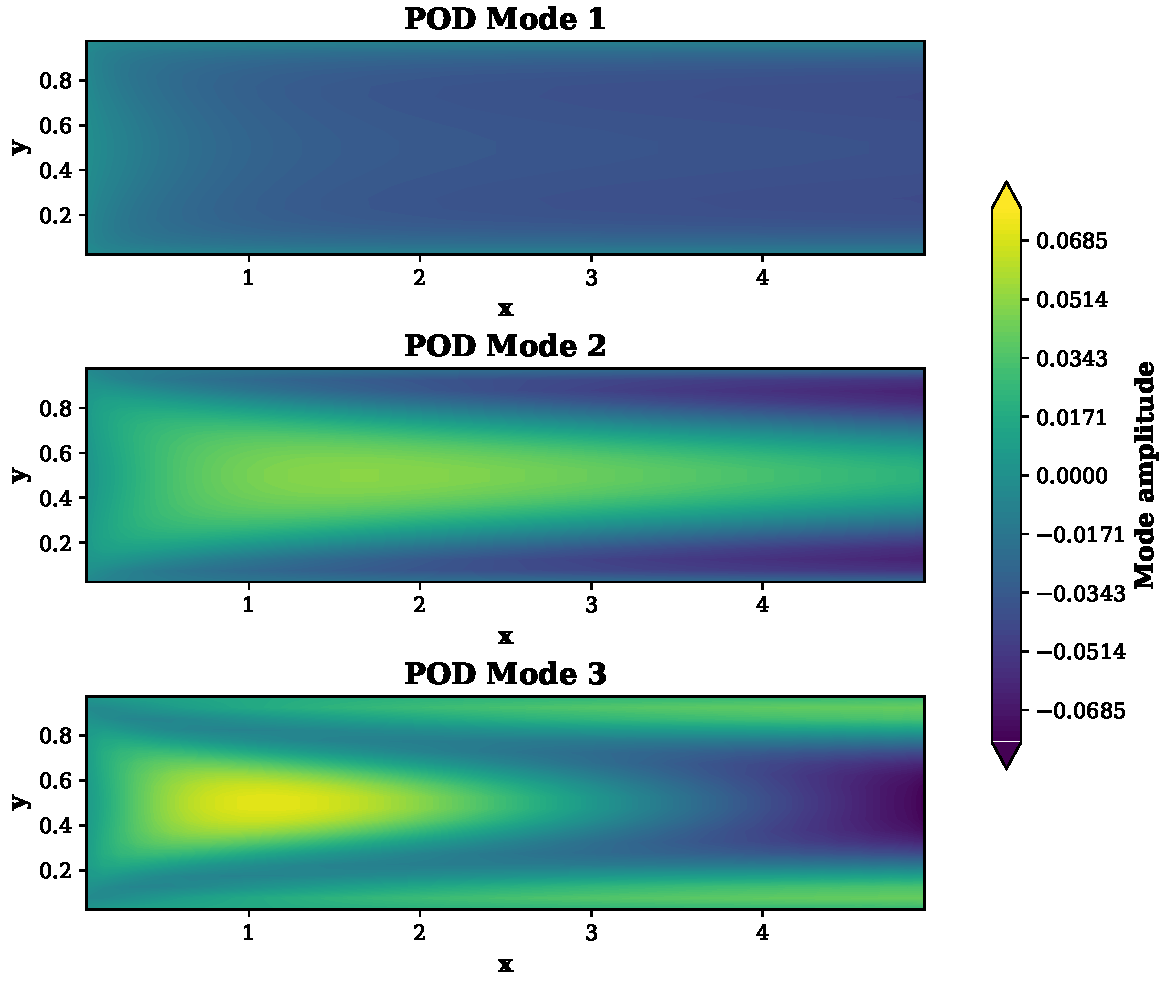
\includegraphics[width=0.95\textwidth]{figures/POD_modes.pdf}
    \caption{First three spatial POD modes obtained from
    the preliminary 25-snapshot dataset.}
    \label{fig:initial_pod_modes}
\end{figure}

The reconstruction accuracy was evaluated by projecting
the original snapshots onto the retained POD basis and
calculating the relative $L_2$ error for each case:
\begin{equation}
    \epsilon_k
    =
    \frac{
    \left\|
    \boldsymbol{\theta}_k
    -
    \hat{\boldsymbol{\theta}}_k
    \right\|_2
    }{
    \left\|
    \boldsymbol{\theta}_k
    \right\|_2
    },
    \label{eq:preliminary_pod_reconstruction_error}
\end{equation}
where $\boldsymbol{\theta}_k$ is the original
temperature-deviation snapshot and
$\hat{\boldsymbol{\theta}}_k$ is its POD reconstruction.
This measure evaluates the ability of the retained modes
to represent the snapshots used to construct the basis.

The reconstruction errors for the 25 cases are summarized
in Table~\ref{tab:preliminary_pod_errors}. Since the five
cases associated with each value of $\mu$ have identical
reported errors, the results are grouped according to
$\mu$ to avoid repeating the same values.

\begin{table}[htbp]
    \centering
    \caption{POD reconstruction errors for the preliminary
    25-case training dataset.}
    \label{tab:preliminary_pod_errors}
    \begin{tabular}{cccc}
        \toprule
        \textbf{$\mu$} &
        \textbf{Case IDs} &
        \textbf{$Br$ range} &
        \textbf{Relative $L_2$ error} \\
        \midrule
        1      & 1--5   & 0.01--2.00 & $4.96\times10^{-5}$ \\
        25.75  & 6--10  & 0.01--2.00 & $4.924\times10^{-3}$ \\
        50.50  & 11--15 & 0.01--2.00 & $1.7011\times10^{-2}$ \\
        75.25  & 16--20 & 0.01--2.00 & $3.284\times10^{-3}$ \\
        100    & 21--25 & 0.01--2.00 & $2.0632\times10^{-2}$ \\
        \bottomrule
    \end{tabular}
\end{table}

The minimum reconstruction error is
$4.96\times10^{-5}$, corresponding to cases 1--5
at $\mu=1$. The maximum error is
$2.0632\times10^{-2}$, corresponding to cases 21--25
at $\mu=100$. These values indicate that the
reconstruction accuracy varies across the sampled
values of $\mu$. The error does not increase
monotonically with $\mu$: it increases from the
lowest parameter value to $\mu=50.5$, decreases at
$\mu=75.25$, and reaches its maximum at $\mu=100$.

An additional observation is that the reconstruction
error remains identical across the five $Br$ values
for each fixed $\mu$. This behavior is consistent
with the linear structure of the steady reduced
governing equation. When the lifting residual is
zero or negligible, the temperature-deviation
equation has a source term proportional to $Br$.
Consequently, for a fixed $\mu$, the deviation
solutions scale linearly with $Br$. Both the
reconstruction error and the norm of the original
deviation field then scale proportionally, leaving
their relative ratio unchanged. The observed
repetition of the reconstruction errors across
different Brinkman numbers is consistent with
this property.

Figure~\ref{fig:preliminary_pod_reconstruction}
compares the full-order temperature fields, their
POD reconstructions, and the corresponding error
fields for representative minimum- and
maximum-error cases. Case 1 represents the
minimum-error group, while case 21 represents
the maximum-error group. Each of these cases has
the same reconstruction error as the other four
cases sharing its value of $\mu$.

\begin{figure}[htbp]
    \centering
    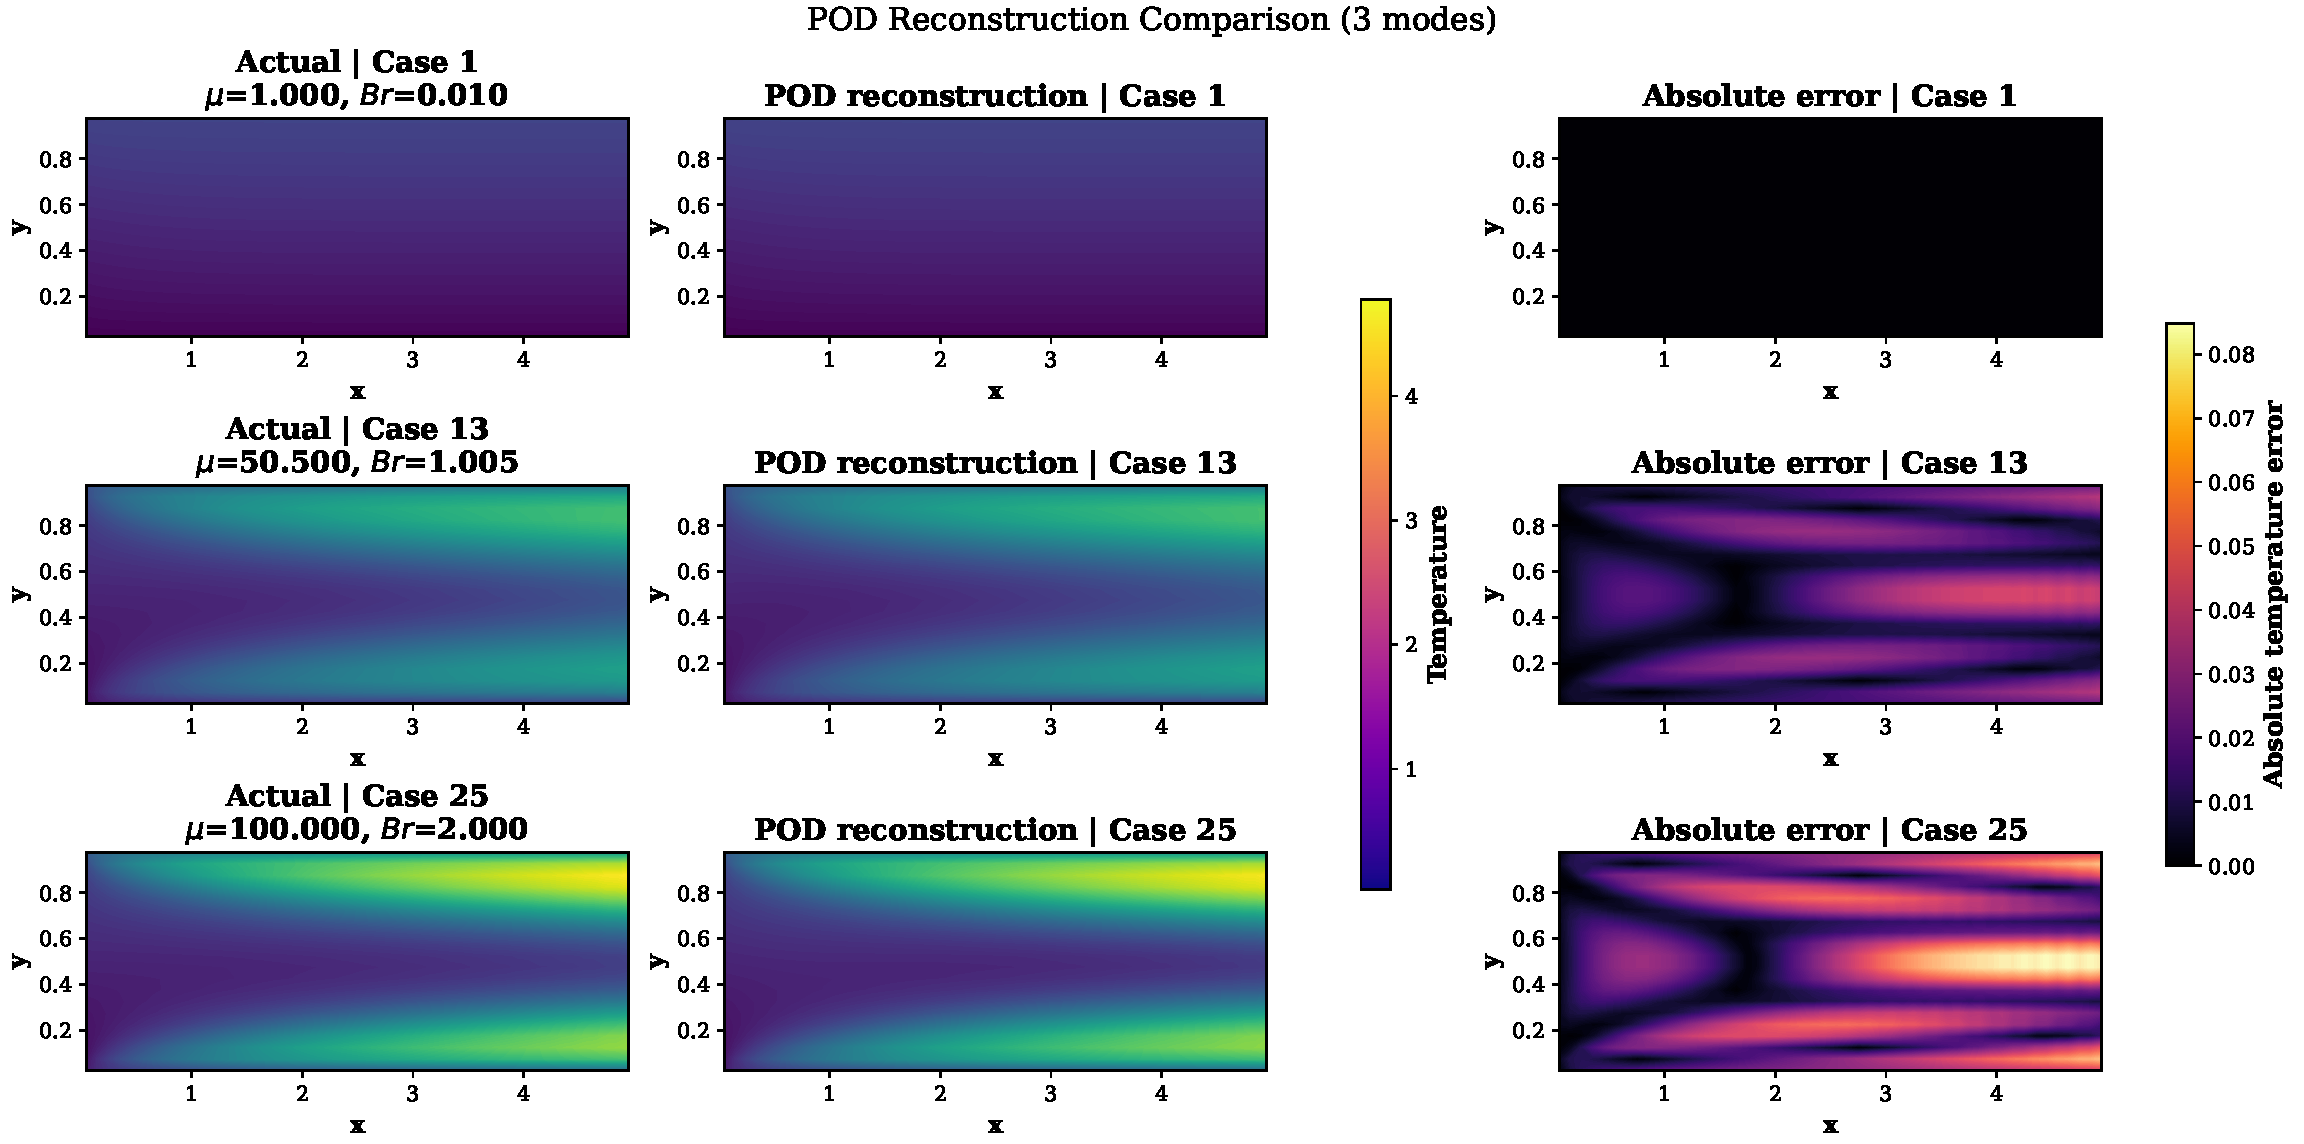
\includegraphics[width=\textwidth]
    {figures/POD_reconstruction.pdf}
    \caption{Comparison of the full-order temperature
    fields, POD reconstructions, and corresponding
    error fields for representative minimum-error
    and maximum-error cases from the preliminary
    25-case dataset.}
    \label{fig:preliminary_pod_reconstruction}
\end{figure}

The reconstruction plots provide a spatial comparison
of the original and approximated temperature fields.
The minimum-error case exhibits very close agreement
between the full-order and reconstructed fields,
whereas the maximum-error case has a larger
reconstruction discrepancy.

These results characterize the ability of the
initial POD basis to represent its own training
snapshots. They do not establish its accuracy at
parameter combinations outside the training dataset.
That question requires evaluating the reduced-order
model at independent parameter values, which is
examined in the following sections.

\subsection{Galerkin ROM results using the 100-snapshot POD basis}
\label{subsec:galerkin_rom_results}

The Galerkin reduced-order model was constructed using the
POD basis obtained from the 100 full-order training
solutions. As reported in Table~\ref{tab:pod_energy}, the
singular values exhibit a rapid decay. The first mode
accounts for 92.6360\% of the total snapshot energy, while
the first three modes capture 99.9833\%. Retaining four
modes increases the cumulative energy to 99.9995\%.

These results indicate that the training snapshots can
be represented using a relatively small number of spatial
modes. However, the accuracy of the Galerkin ROM also
depends on how well the reduced governing equations
determine the modal coefficients. Therefore, the ROM
temperature fields are compared directly with their
corresponding full-order solutions.

The ROM was evaluated for the 100 parameter combinations
in the original training dataset. For each case, the
Galerkin-projected system was solved, and the resulting
modal coefficients were used to reconstruct the complete
temperature field:
\[
\mathbf{T}_{\mathrm{ROM}}
=
\mathbf{T}_{\mathrm{ref}}+\mathbf{V}_r\mathbf{a}.
\]
The reconstructed fields were compared with the
corresponding full-order temperature solutions using
the relative discrete $L_2$ error, RMSE, and maximum
absolute error defined in the previous section.

The aggregate error statistics are reported in
Table~\ref{tab:initial_galerkin_errors}.

\begin{table}[htbp]
    \centering
    \caption{Aggregate Galerkin ROM errors over the
    100 training cases.}
    \label{tab:initial_galerkin_errors}
    \begin{tabular}{lc}
        \toprule
        \textbf{Metric} & \textbf{Value} \\
        \midrule
        Successful cases & 100 \\
        Mean relative $L_2$ error & $2.401402\times10^{-2}$ \\
        Median relative $L_2$ error & $1.705007\times10^{-2}$ \\
        Maximum relative $L_2$ error & $1.262083\times10^{-1}$ \\
        Mean RMSE & $6.498504\times10^{-2}$ \\
        Mean maximum absolute error & $1.353265\times10^{-1}$ \\
        \bottomrule
    \end{tabular}
\end{table}

The mean relative $L_2$ error across the 100 cases is
approximately 2.40\%, while the median error is
approximately 1.71\%. The maximum error reaches
approximately 12.62\%. The difference between the mean
and median indicates that the error distribution is
not uniform across the evaluated cases. Although most
cases have relatively small errors, some parameter
combinations produce considerably larger discrepancies.

The cases with the minimum and maximum relative
$L_2$ errors are summarized in
Table~\ref{tab:initial_galerkin_extremes}.

\begin{table}[htbp]
    \centering
    \caption{Minimum- and maximum-error cases in the
    initial Galerkin ROM evaluation.}
    \label{tab:initial_galerkin_extremes}
    \begin{tabular}{ccc}
        \toprule
        \textbf{Case} &
        \textbf{Relative $L_2$ error} &
        \textbf{Result} \\
        \midrule
        \texttt{train\_0001} &
        $7.040618\times10^{-6}$ &
        Minimum error \\
        \texttt{train\_0020} &
        $1.262083\times10^{-1}$ &
        Maximum error \\
        \bottomrule
    \end{tabular}
\end{table}

The minimum-error case has a relative $L_2$ error of
approximately $0.000704\%$, indicating very close
agreement between the full-order and reduced-order
temperature fields. In contrast, the maximum-error
case has a relative error of approximately 12.62\%.
This difference illustrates that the accuracy of the
reduced model varies across the parameter combinations,
even when the same POD basis and reduced formulation
are used.

Figures~\ref{fig:galerkin_minimum_error} and
\ref{fig:galerkin_maximum_error} present the spatial
comparison for the two cases. Each figure shows the
full-order temperature field, the reconstructed
Galerkin ROM temperature field, and their difference.

\begin{figure}[htbp]
    \centering
    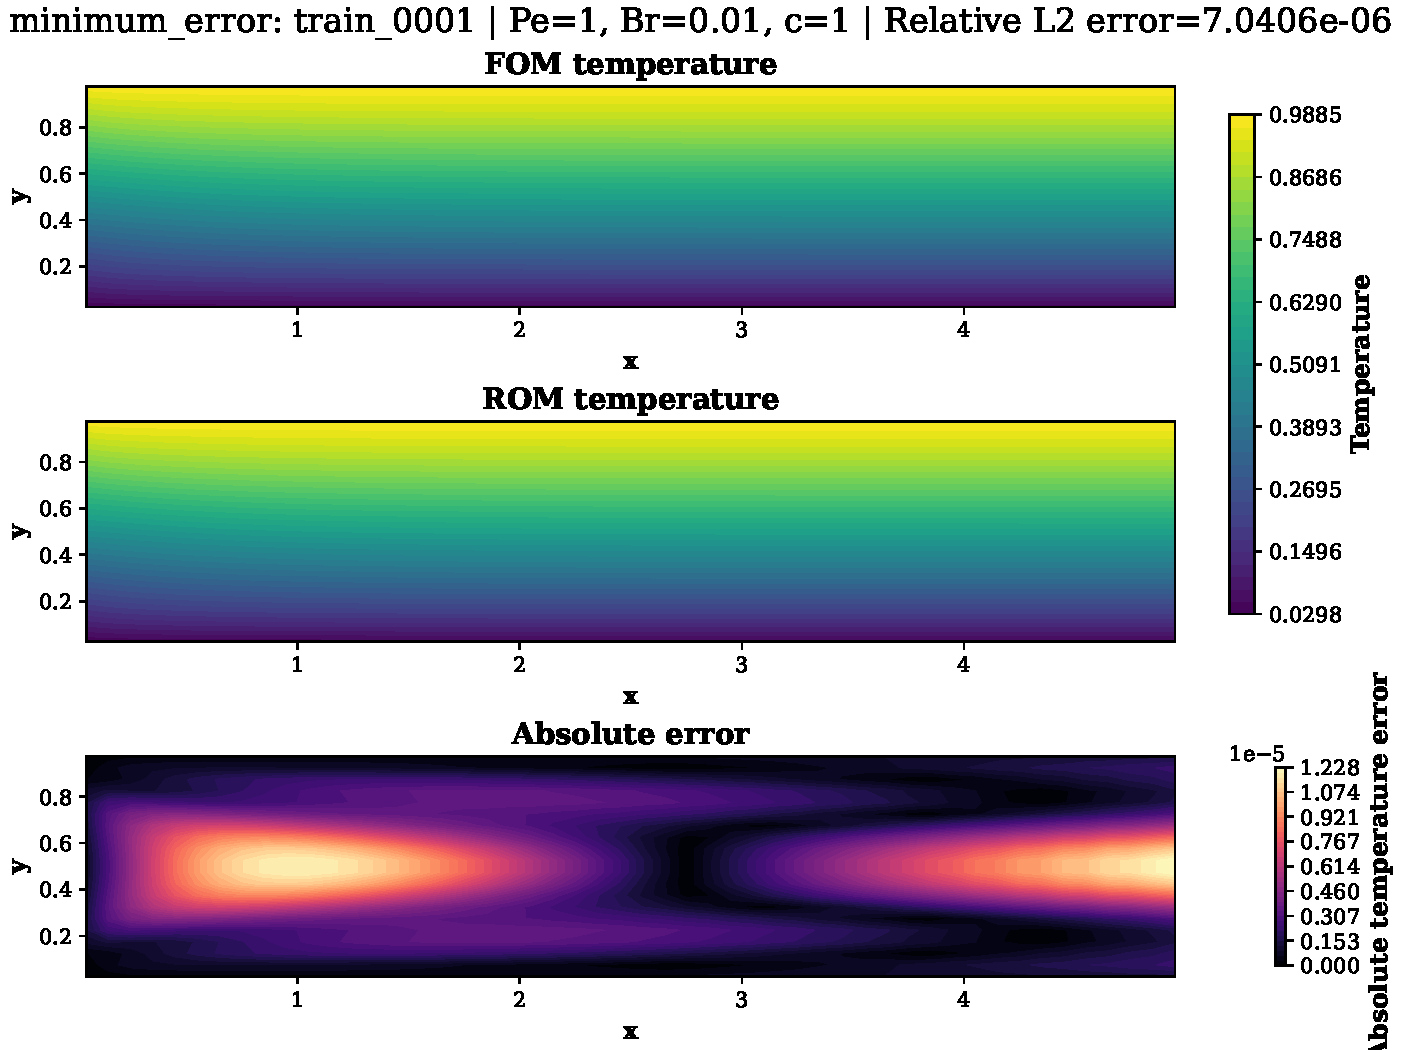
\includegraphics[width=\textwidth]
    {figures/Galerkin_minimum_error.pdf}
    \caption{Full-order temperature field, Galerkin ROM
    reconstruction, and corresponding error field for
    the minimum-error case (\texttt{train\_0001}).}
    \label{fig:galerkin_minimum_error}
\end{figure}

The comparison of the two cases provides a spatial
interpretation of the aggregate error statistics.
The minimum-error reconstruction exhibits close
agreement with the full-order solution, whereas the
maximum-error case displays larger discrepancies
between the two fields.

It should be noted that these 100 parameter combinations
were also used to construct the original POD basis.
Therefore, although the results assess the accuracy
of the Galerkin equations and their reconstructed
temperature fields at the training parameter values,
they do not constitute an independent assessment of
prediction accuracy at unseen parameter combinations.
The latter is examined using the separate test
dataset in the subsequent evaluation.

\begin{figure}[htbp]
    \centering
    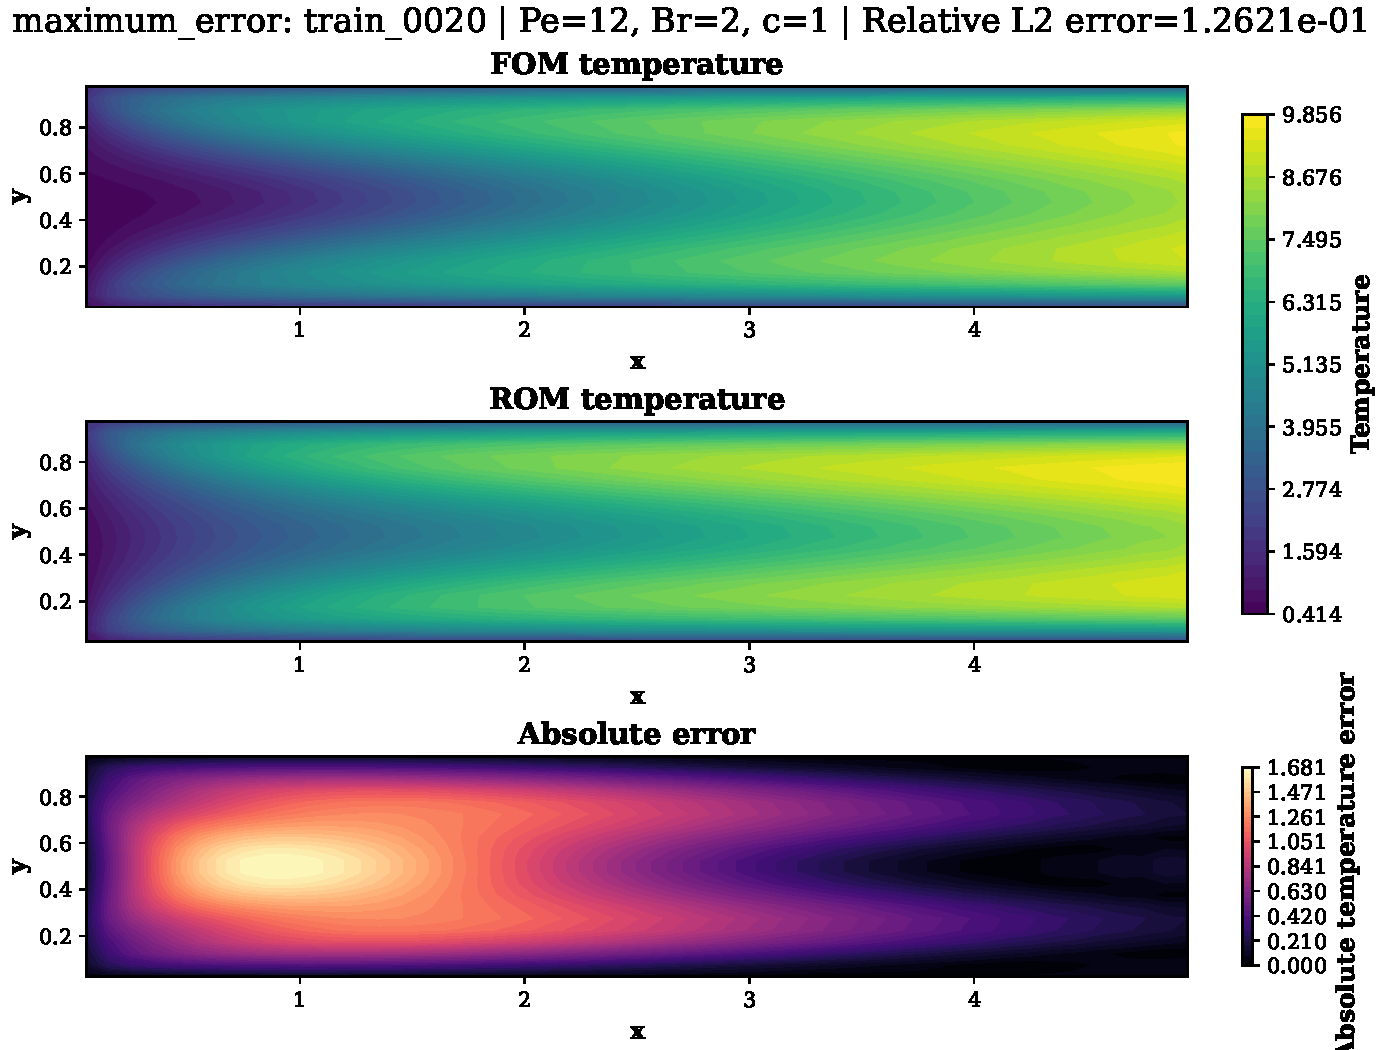
\includegraphics[width=\textwidth]
    {figures/Galerkin_maximum_error.pdf}
    \caption{Full-order temperature field, Galerkin ROM
    reconstruction, and corresponding error field for
    the maximum-error case (\texttt{train\_0020}).}
    \label{fig:galerkin_maximum_error}
\end{figure}


\subsection{Initial LHS evaluation and mode-count study}
\label{subsec:lhs_mode_count_results}

The first stage of ROM refinement examines the predictive
accuracy of the original POD basis using an independent
Latin hypercube sampling (LHS) dataset. This dataset
contains 100 parameter combinations within the prescribed
domain:
\[
1\leq\mu\leq100,
\qquad
0.01\leq Br\leq2.
\]
For each parameter combination, a full-order simulation
is performed to provide a reference temperature field.
The original POD basis is then evaluated using the
Galerkin reduced-order model.

The purpose of this evaluation is to identify the
dependence of ROM accuracy on the number of retained
POD modes and to locate regions of the parameter domain
where the original basis produces relatively large
errors. The resulting error records are subsequently
used to guide the selection of additional training
snapshots.

\paragraph{Effect of the retained basis dimension.}

The original POD basis is evaluated using the mode
counts
\[
r\in\{1,2,3,4,5,6,8,10\}.
\]
For each mode count, the first $r$ spatial modes are
retained, and the corresponding Galerkin reduced system
is solved for all 100 LHS cases. The relative $L_2$
error, RMSE, and maximum error are calculated for each
case. The aggregate statistics are reported in
Table~\ref{tab:lhs_mode_count_results}.

\begin{table}[htbp]
    \centering
    \caption{ROM error statistics for different retained
    POD mode counts over the 100 LHS screening cases.}
    \label{tab:lhs_mode_count_results}
    \scriptsize
    \setlength{\tabcolsep}{4pt}
    \begin{tabular}{ccccccc}
        \toprule
        \textbf{Modes} &
        \textbf{Cases} &
        \textbf{Mean error} &
        \textbf{Median error} &
        \textbf{95th percentile} &
        \textbf{Maximum error} &
        \textbf{Mean RMSE} \\
        \midrule
        1  & 100 & 0.395587 & 0.418291 & 0.614300 & 0.636144 & 0.813243 \\
        2  & 100 & 0.171552 & 0.175393 & 0.348644 & 0.410623 & 0.378429 \\
        3  & 100 & 0.027889 & 0.025590 & 0.063268 & 0.079345 & 0.073850 \\
        4  & 100 & 0.007663 & 0.006444 & 0.020409 & 0.044846 & 0.024056 \\
        5  & 100 & 0.002532 & 0.001145 & 0.013146 & 0.031450 & 0.010355 \\
        6  & 100 & 0.001377 & 0.000184 & 0.008551 & 0.024884 & 0.006698 \\
        8  & 100 & 0.000726 & $3.02\times10^{-6}$ & 0.005354 & 0.015513 & 0.003776 \\
        10 & 100 & 0.000468 & $2.96\times10^{-8}$ & 0.003338 & 0.010435 & 0.002440 \\
        \bottomrule
    \end{tabular}
\end{table}

The results show a substantial reduction in ROM error
as the number of retained modes increases. With one
mode, the mean relative $L_2$ error is approximately
39.56\%, and the maximum error reaches 63.61\%.
Increasing the basis dimension to three modes reduces
the mean error to 2.79\%. With four modes, the mean
error decreases further to approximately 0.77\%.

The improvement continues with additional modes.
For ten retained modes, the mean relative $L_2$ error
is approximately 0.0468\%, while the maximum error
decreases to approximately 1.04\%. The 95th-percentile
error also decreases from 61.43\% with one mode to
approximately 0.334\% with ten modes.

The median error at ten modes is particularly small,
approximately $2.96\times10^{-8}$. However, the
maximum error remains considerably larger than the
median. This indicates that the ROM does not achieve
uniformly similar accuracy across all parameter
combinations, even when a relatively large number
of modes is retained.

Figure~\ref{fig:mode_count_error_statistics} presents
the variation of the mean, median, 95th-percentile,
and maximum relative $L_2$ errors with the number of
retained modes.

\begin{figure}[htbp]
    \centering
    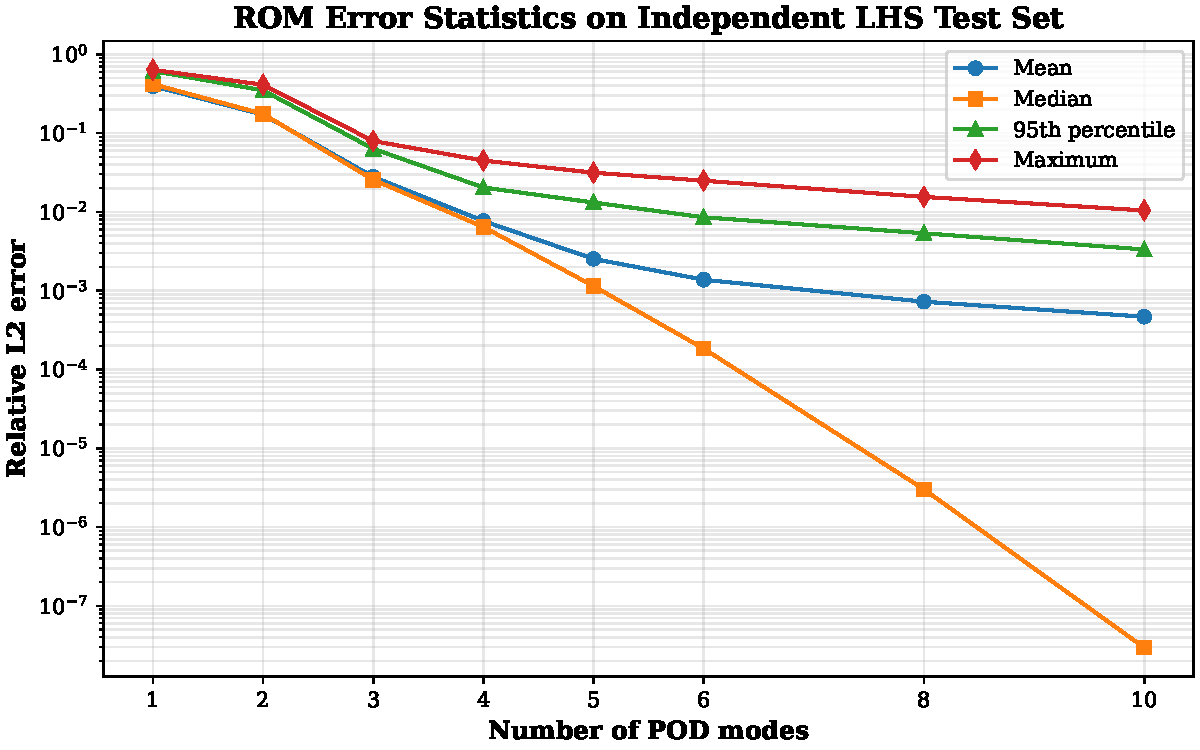
\includegraphics[width=0.95\textwidth]
    {figures/mode_count_study_error_statistics.pdf}
    \caption{Mean, median, 95th-percentile, and maximum
    relative $L_2$ errors as functions of the number
    of retained POD modes for the 100 LHS screening cases.}
    \label{fig:mode_count_error_statistics}
\end{figure}

The decreasing error statistics confirm that increasing
the reduced basis dimension improves the overall
accuracy of the original Galerkin ROM over the sampled
parameter domain. Nevertheless, the differences
between the median and maximum errors suggest that
some parameter regions remain more difficult to
represent than others. Therefore, increasing the
number of modes alone does not fully address the
spatially localized deficiencies of the original basis.

\paragraph{Error distribution in the parameter domain.}

To examine where the ROM produces relatively large
errors, the case-wise relative $L_2$ errors are also
visualized over the two-dimensional parameter space.
Each LHS case is associated with its parameter
coordinates $(\mu,Br)$ and its corresponding ROM
error.

Since the LHS parameter combinations are irregularly
distributed, they do not form a structured rectangular
grid. Therefore, a triangulation-based visualization
is used to represent the error distribution. The
sample points are connected through a triangular
mesh, and the error values are interpolated over the
resulting triangular regions to construct a
contour-like map.

Figure~\ref{fig:lhs_triangulated_error} presents
the resulting spatial distribution of the relative
$L_2$ error across the parameter domain.

\begin{figure}[htbp]
    \centering
    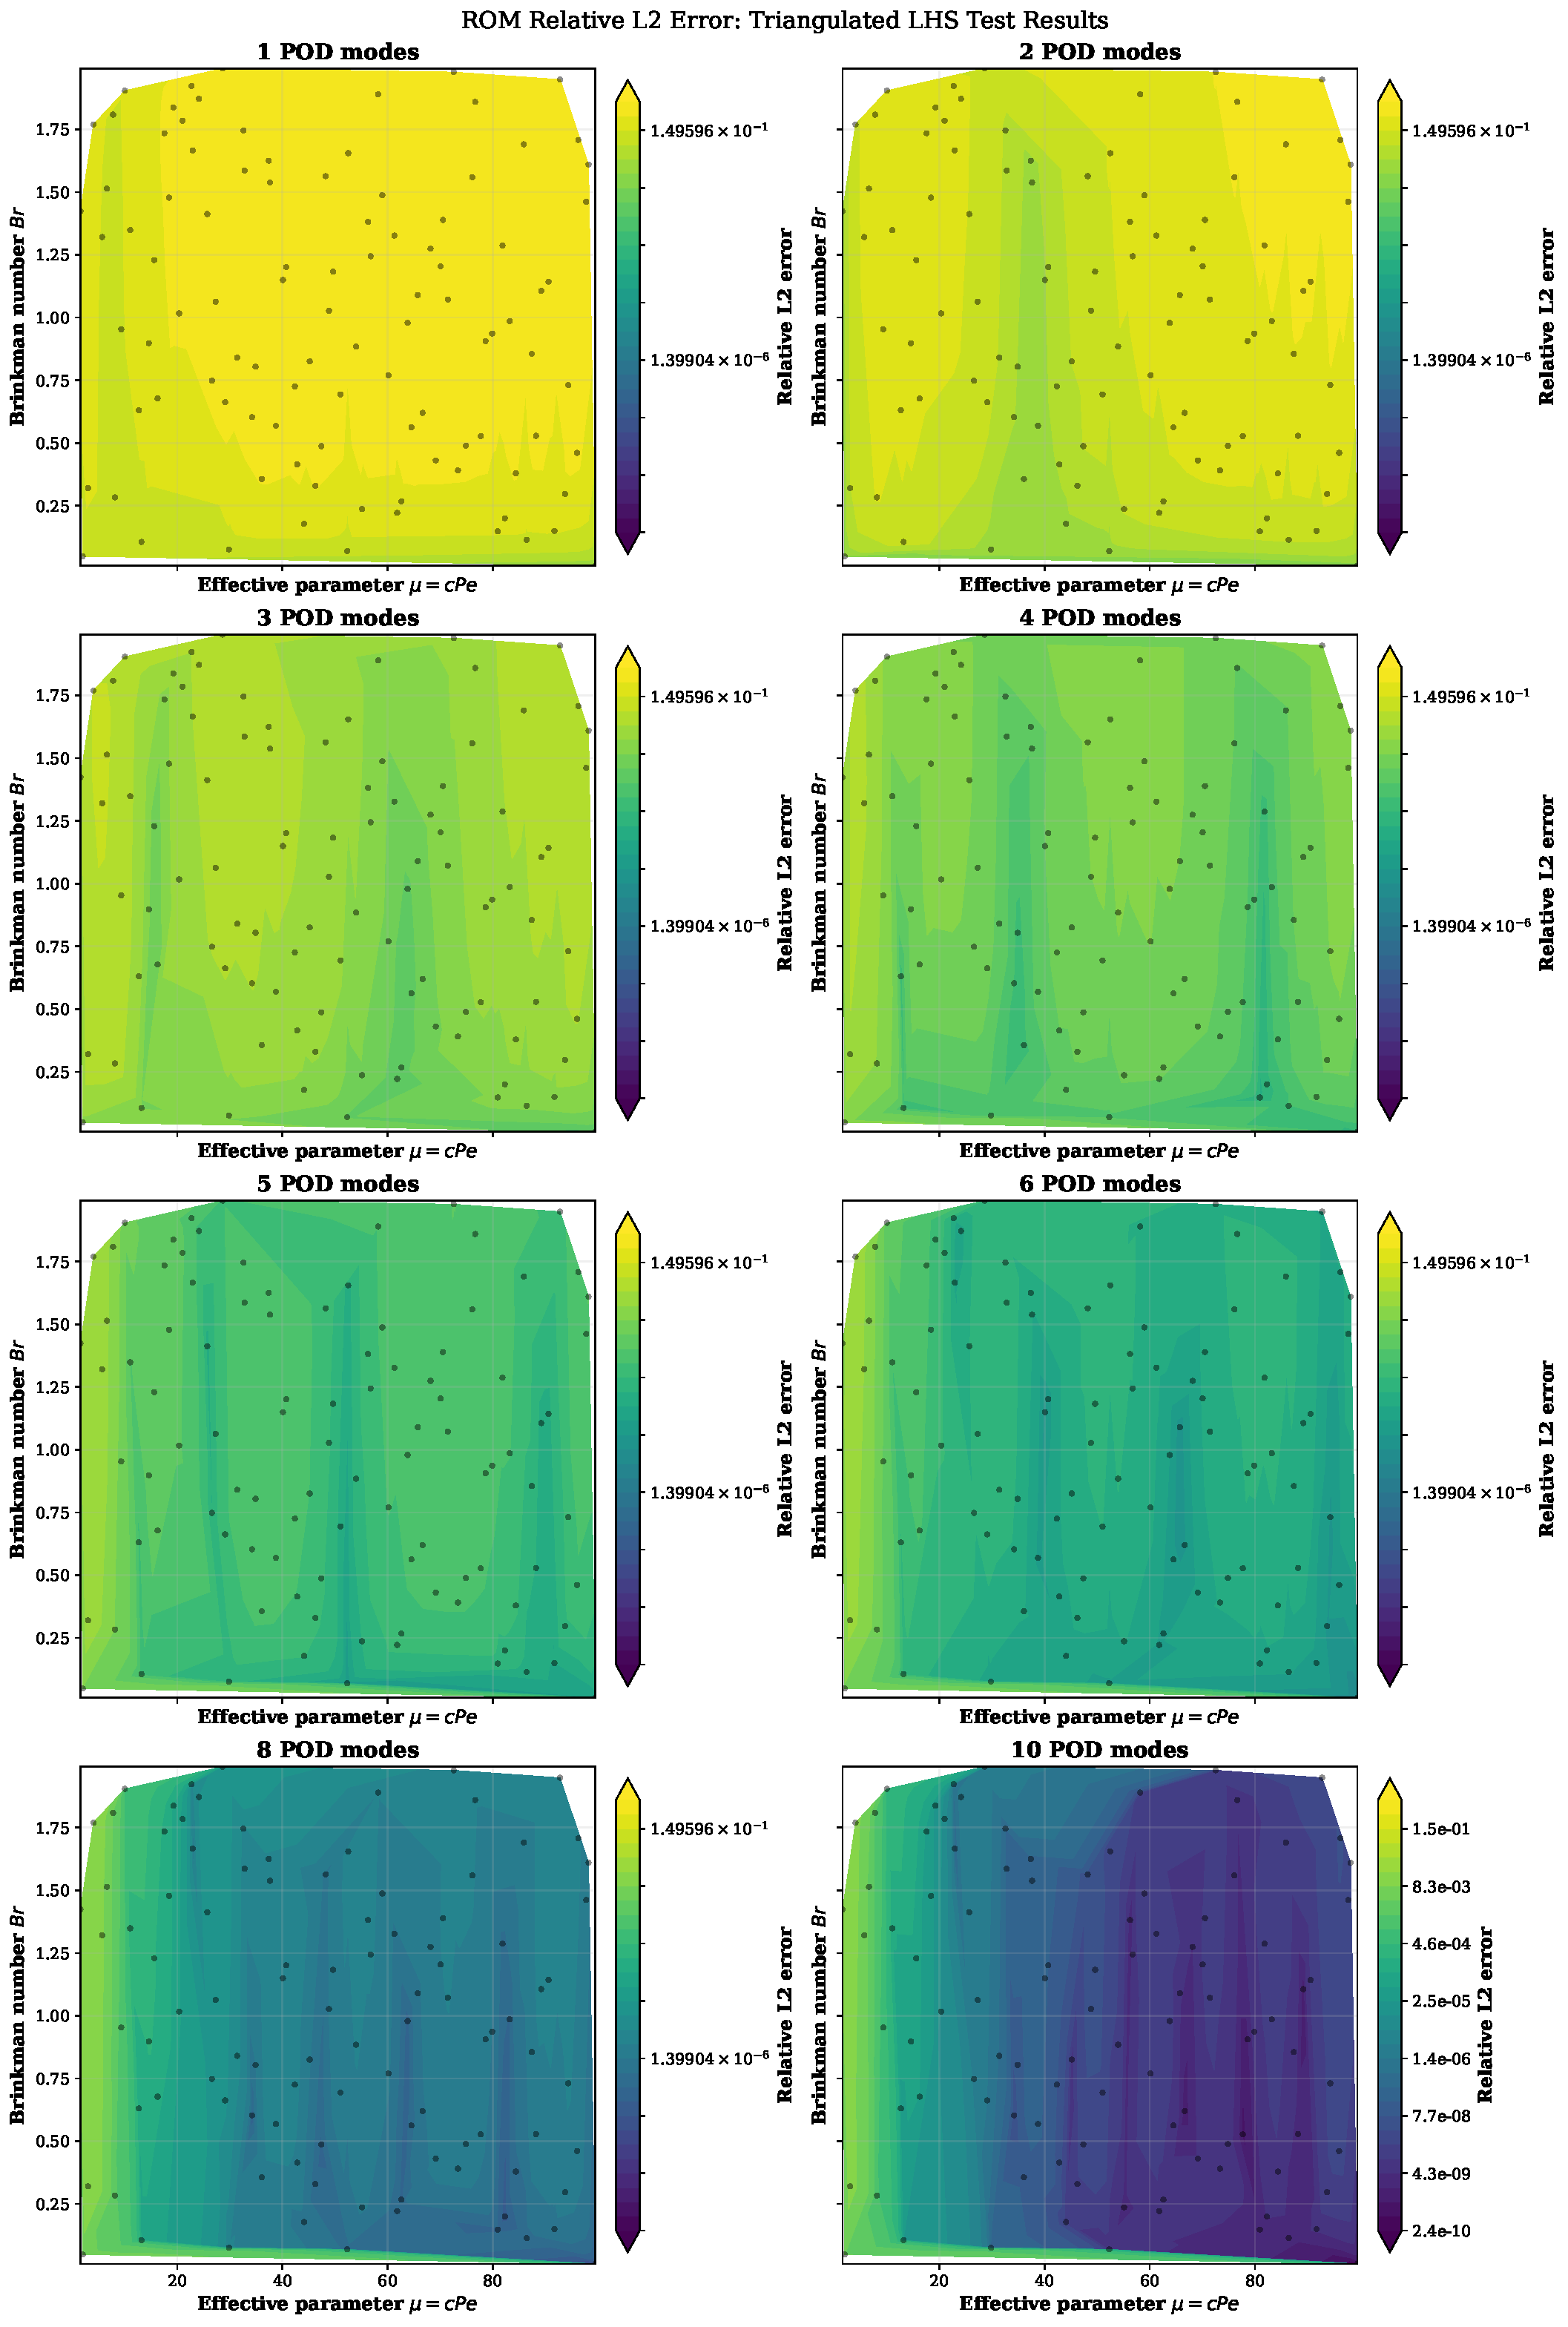
\includegraphics[width=0.95\textwidth]
    {figures/relative_l2_error_triangulated_lhs.pdf}
    \caption{Triangulation-based visualization of the
    relative $L_2$ ROM error over the 100 LHS
    parameter combinations.}
    \label{fig:lhs_triangulated_error}
\end{figure}

The triangulated map provides a visual representation
of the variation in ROM accuracy across the sampled
parameter domain. Regions associated with larger
errors can be identified and examined to determine
where additional training snapshots may be useful.
The interpolated regions are intended as a
visualization of the sampled error data; they do
not represent additional ROM evaluations between
the LHS points.

The mode-count statistics and parameter-space
visualization together provide the basis for the
subsequent snapshot-enrichment procedure. Rather than
increasing the training dataset uniformly, the
following refinement stage selects candidate
parameter combinations from the high-error cases
and generates additional full-order snapshots
around the selected locations.

\subsection{Snapshot enrichment and construction of the augmented basis}
\label{subsec:augmented_basis_results}

The high-error regions identified during the initial LHS
screening were used to generate additional full-order
snapshots. The hotspot-selection procedure identified
three parameter-space locations, around which local
parameter grids were constructed. After applying the
parameter-domain restrictions, removing duplicate
combinations, and excluding cases already present in
the original training grid, 15 additional parameter
combinations were obtained.

All 15 additional full-order simulations converged
successfully. No nonconverged cases or simulation
errors were reported. The resulting snapshot matrix
has dimensions $1000\times15$, as summarized in
Table~\ref{tab:enrichment_generation_results}.

\begin{table}[htbp]
    \centering
    \caption{Results of the additional snapshot-generation
    procedure.}
    \label{tab:enrichment_generation_results}
    \begin{tabular}{lc}
        \toprule
        \textbf{Quantity} & \textbf{Result} \\
        \midrule
        Selected hotspot centres & 3 \\
        Generated parameter combinations & 15 \\
        Successful full-order simulations & 15 \\
        Nonconverged simulations & 0 \\
        Cases with simulation errors & 0 \\
        Additional snapshot matrix dimensions & $1000\times15$ \\
        \bottomrule
    \end{tabular}
\end{table}

The additional snapshots were combined with the original
100 snapshots to construct the augmented snapshot matrix:
\[
\mathbf{X}_{\mathrm{aug}}
=
\begin{bmatrix}
\mathbf{X}_{\mathrm{original}} &
\mathbf{X}_{\mathrm{additional}}
\end{bmatrix}.
\]
Therefore,
\[
\mathbf{X}_{\mathrm{aug}}
\in\mathbb{R}^{1000\times115}.
\]
A new SVD was performed on this combined matrix, and
the augmented POD basis was obtained from its left
singular vectors.

The three-mode cumulative POD energy of the augmented
basis is 99.9699\%, compared with 99.9833\% for the
original basis. Although the augmented basis has a
slightly lower cumulative energy at this mode count,
this does not directly indicate poorer predictive
accuracy. The additional snapshots change the total
snapshot energy and its distribution among the modes.
The effect of enrichment must therefore be judged
through the subsequent ROM evaluation on independent
parameter combinations.

\subsection{Independent comparison of the original and augmented bases}
\label{subsec:original_augmented_comparison}

The final comparison was performed using a separate
set of 100 LHS parameter combinations. These cases
were generated after construction of the augmented
basis. Parameter combinations already present in
either the original or augmented training datasets
were excluded. The full-order solver was then executed
for each accepted test case to obtain its reference
temperature field.

Both POD bases were evaluated using exactly the same
100 test cases and the same eight retained mode counts:
\[
r\in\{1,2,3,4,5,6,8,10\}.
\]
For each test case and mode count, the original-basis
ROM and augmented-basis ROM were solved and compared
against the same full-order temperature field. This
resulted in
\[
2\times100\times8=1600
\]
ROM evaluations.

The comparison therefore changes the POD basis while
keeping the test cases, reference solutions, mode
counts, and error definitions fixed.

\paragraph{Comparison of aggregate error statistics.}

Table~\ref{tab:final_basis_error_statistics} reports
the relative $L_2$ error distributions for the two
bases. The mean, median, 95th-percentile, and maximum
errors are included for each retained mode count.

\begin{table}[htbp]
    \centering
    \caption{Relative $L_2$ error statistics for the
    original and augmented POD bases over 100 independent
    test cases.}
    \label{tab:final_basis_error_statistics}
    \scriptsize
    \setlength{\tabcolsep}{3pt}
    \resizebox{\textwidth}{!}{%
        \begin{tabular}{ccccccc}
            \toprule
            \textbf{Basis} &
            \textbf{Modes} &
            \textbf{Cases} &
            \textbf{Mean} &
            \textbf{Median} &
            \textbf{95th percentile} &
            \textbf{Maximum} \\
            \midrule
            Original  & 1  & 100 & 0.401768 & 0.437246 & 0.620615 & 0.634832 \\
            Original  & 2  & 100 & 0.176187 & 0.166973 & 0.371498 & 0.411629 \\
            Original  & 3  & 100 & 0.028506 & 0.024564 & 0.062156 & 0.081035 \\
            Original  & 4  & 100 & 0.008127 & 0.007205 & 0.026946 & 0.044410 \\
            Original  & 5  & 100 & 0.002725 & 0.001065 & 0.018959 & 0.030992 \\
            Original  & 6  & 100 & 0.001571 & 0.000189 & 0.013137 & 0.026048 \\
            Original  & 8  & 100 & 0.000876 & $3.00\times10^{-6}$ & 0.006426 & 0.018205 \\
            Original  & 10 & 100 & 0.000577 & $3.31\times10^{-8}$ & 0.003450 & 0.013008 \\
            \midrule
            Augmented & 1  & 100 & 0.384505 & 0.423167 & 0.594550 & 0.608058 \\
            Augmented & 2  & 100 & 0.193602 & 0.163706 & 0.435441 & 0.468897 \\
            Augmented & 3  & 100 & 0.036678 & 0.035301 & 0.079193 & 0.095283 \\
            Augmented & 4  & 100 & 0.013629 & 0.013465 & 0.028654 & 0.037714 \\
            Augmented & 5  & 100 & 0.003841 & 0.004188 & 0.007181 & 0.009805 \\
            Augmented & 6  & 100 & 0.000930 & 0.000758 & 0.001740 & 0.005040 \\
            Augmented & 8  & 100 & 0.000141 & 0.000123 & 0.000241 & 0.001747 \\
            Augmented & 10 & 100 & $1.74\times10^{-5}$ & $1.30\times10^{-5}$ & $3.07\times10^{-5}$ & 0.000401 \\
            \bottomrule
        \end{tabular}%
    }
\end{table}

For one retained mode, the augmented basis reduces
the mean relative $L_2$ error from 0.401768 to
0.384505. The improvement is modest, but it is
observed across all 100 test cases.

For two and three modes, however, the augmented basis
produces higher mean and maximum errors. The mean
relative $L_2$ error increases from 0.176187 to
0.193602 for two modes and from 0.028506 to 0.036678
for three modes. The maximum errors also increase
at both ranks.

A similar increase in mean error occurs for four
and five modes. However, the maximum error decreases
at both mode counts. For four modes, it decreases
from 0.044410 to 0.037714. For five modes, it
decreases more substantially, from 0.030992 to
0.009805. Thus, the enrichment reduces the largest
observed errors at these ranks, although the mean
error becomes higher.

The behavior changes at six modes. The augmented
basis reduces the mean relative $L_2$ error from
0.001571 to 0.000930 and the maximum error from
0.026048 to 0.005040. These reductions become
more pronounced at eight and ten modes.

At ten modes, the mean relative $L_2$ error decreases
from 0.000577 to $1.74\times10^{-5}$, while the
maximum error decreases from 0.013008 to 0.000401.
The corresponding reductions are approximately
96.98\% and 96.92\%, respectively. The 95th-percentile
error also decreases from 0.003450 to
$3.07\times10^{-5}$.

\paragraph{Paired case-wise comparison.}

The aggregate statistics do not indicate how
consistently the augmented basis improves individual
test cases. For this reason, the error difference
is calculated separately for every paired case:
\[
\boxed{
\Delta\epsilon_k
=
\epsilon_{\mathrm{rel},k}^{\mathrm{aug}}
-
\epsilon_{\mathrm{rel},k}^{\mathrm{orig}}.
}
\]
A negative value indicates that the augmented basis
produces a lower error, while a positive value
indicates that the original basis performs better.

The percentage of improved cases is calculated as
\[
P_{\mathrm{improved}}
=
\frac{
N(\Delta\epsilon_k<0)
}{100}
\times100.
\]
The percentage reductions in mean and maximum errors
are also calculated relative to the original basis.

The paired results are summarized in
Table~\ref{tab:paired_enrichment_results}.

\begin{table}[htbp]
    \centering
    \caption{Paired comparison of the original and
    augmented POD bases over 100 independent test cases.}
    \label{tab:paired_enrichment_results}
    \scriptsize
    \setlength{\tabcolsep}{3pt}
    \resizebox{\textwidth}{!}{%
        \begin{tabular}{ccccccccc}
            \toprule
            \textbf{Modes} &
            \textbf{Mean reduction (\%)} &
            \textbf{Max. reduction (\%)} &
            \textbf{Mean $\Delta\epsilon$} &
            \textbf{Median $\Delta\epsilon$} &
            \textbf{5th percentile} &
            \textbf{95th percentile} &
            \textbf{Improved cases (\%)} \\
            \midrule
            1  & 4.2967   & 4.2175   & -0.017260 & -0.017340 & -0.026400 & -0.004820 & 100 \\
            2  & -9.8843  & -13.9125 & 0.017415  & 0.041945  & -0.080070 & 0.077803  & 33 \\
            3  & -28.6650 & -17.5825 & 0.008171  & 0.011487  & -0.027850 & 0.031049  & 32 \\
            4  & -67.6905 & 15.0773  & 0.005501  & 0.007381  & -0.014240 & 0.021053  & 28 \\
            5  & -40.9432 & 68.3639  & 0.001116  & 0.002426  & -0.013540 & 0.005900  & 22 \\
            6  & 40.7665  & 80.6523  & -0.000640 & 0.000445  & -0.011450 & 0.001546  & 22 \\
            8  & 83.9121  & 90.4018  & -0.000730 & 0.000082  & -0.006310 & 0.000193  & 11 \\
            10 & 96.9841  & 96.9175  & -0.000560 & 0.00000833 & -0.003440 & 0.0000271 & 20 \\
            \bottomrule
        \end{tabular}%
    }
\end{table}

For one mode, all test cases improve with the augmented
basis. At two through five modes, the percentage of
improved cases decreases to between 22\% and 33\%.
The positive mean and median case-wise error changes
at these ranks indicate that the augmented basis
generally produces higher errors across the paired
test cases, even though the maximum error is reduced
at four and five modes.

At six, eight, and ten modes, the mean case-wise
error change becomes negative, indicating an overall
reduction when the differences are averaged. However,
the median case-wise change remains positive at all
three mode counts, and the percentage of improved
cases is only 22\%, 11\%, and 20\%, respectively.

This distinction is important. At eight modes, for
example, the mean relative $L_2$ error is reduced
by approximately 83.91\%, yet only 11 of the 100
test cases have lower errors with the augmented
basis. At ten modes, the mean error is reduced by
approximately 96.98\%, while only 20 cases improve.

Therefore, the large reductions in aggregate errors
are concentrated in a relatively small number of
test cases. The errors of the remaining cases
generally increase, but these increases are
outweighed by substantial reductions in a smaller
number of cases. This explains why the mean and
maximum errors can improve while most individual
cases do not.

\paragraph{Spatial distribution of the error changes.}

The paired error distributions are also examined
over the parameter domain. The triangulated error
maps compare the relative $L_2$ errors of the
original and augmented bases at each retained
mode count. These maps help identify whether the
changes in the aggregate statistics are associated
with the parameter regions targeted during
snapshot enrichment.

The error-statistics comparison is shown in
Figure~\ref{fig:original_augmented_error_statistics}.
The corresponding relative error reductions are
shown in Figure~\ref{fig:original_augmented_error_reduction}.

\begin{figure}[htbp]
    \centering
    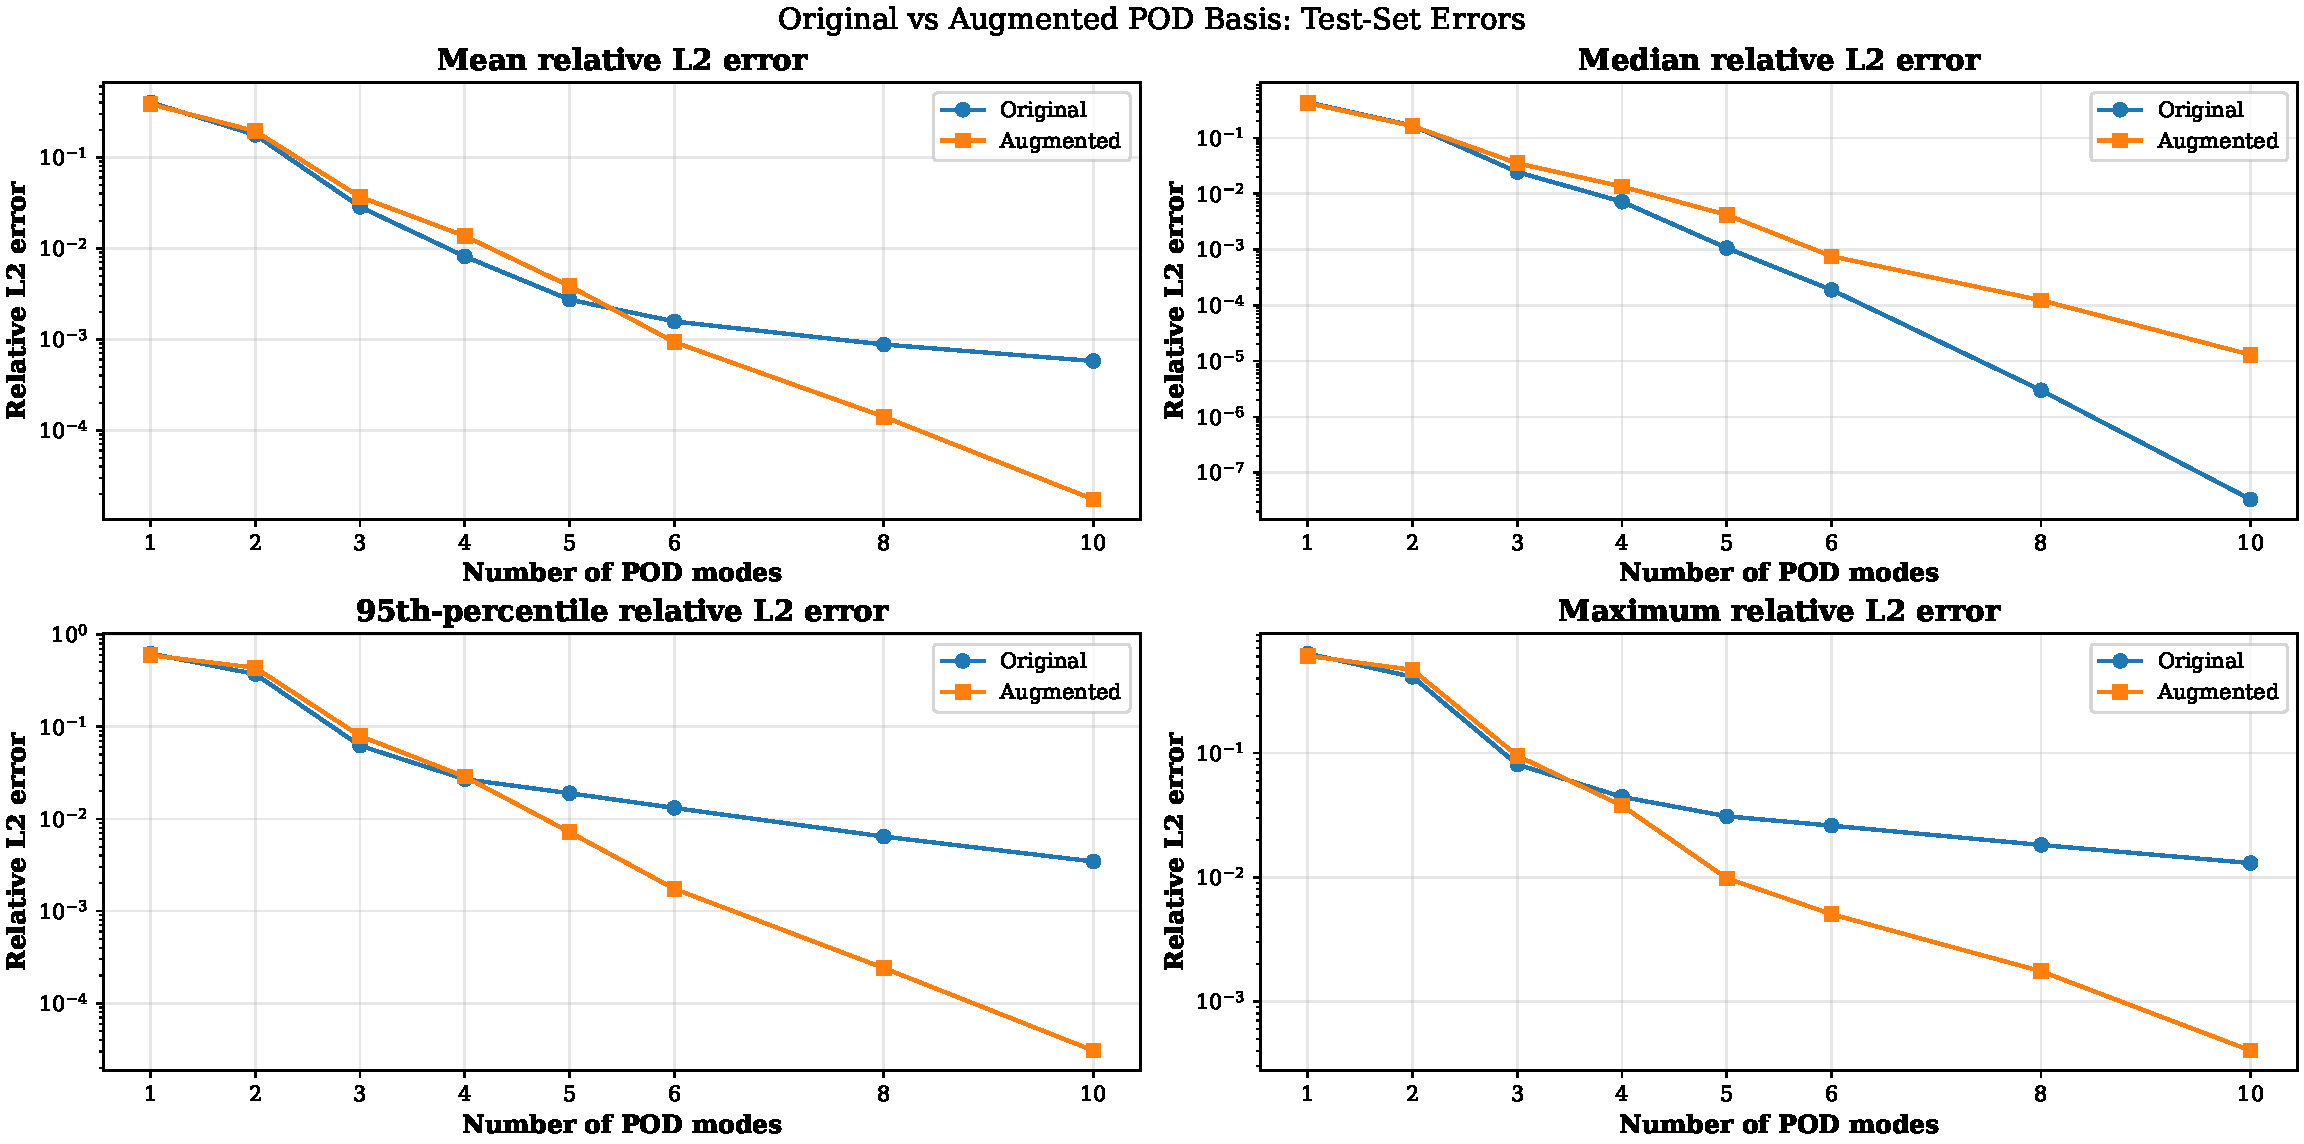
\includegraphics[width=0.95\textwidth]
    {figures/original_augmented_rom_comparison_error_statistics.pdf}
    \caption{Comparison of error statistics for the
    original and augmented POD bases across the
    retained mode counts.}
    \label{fig:original_augmented_error_statistics}
\end{figure}

\begin{figure}[htbp]
    \centering
    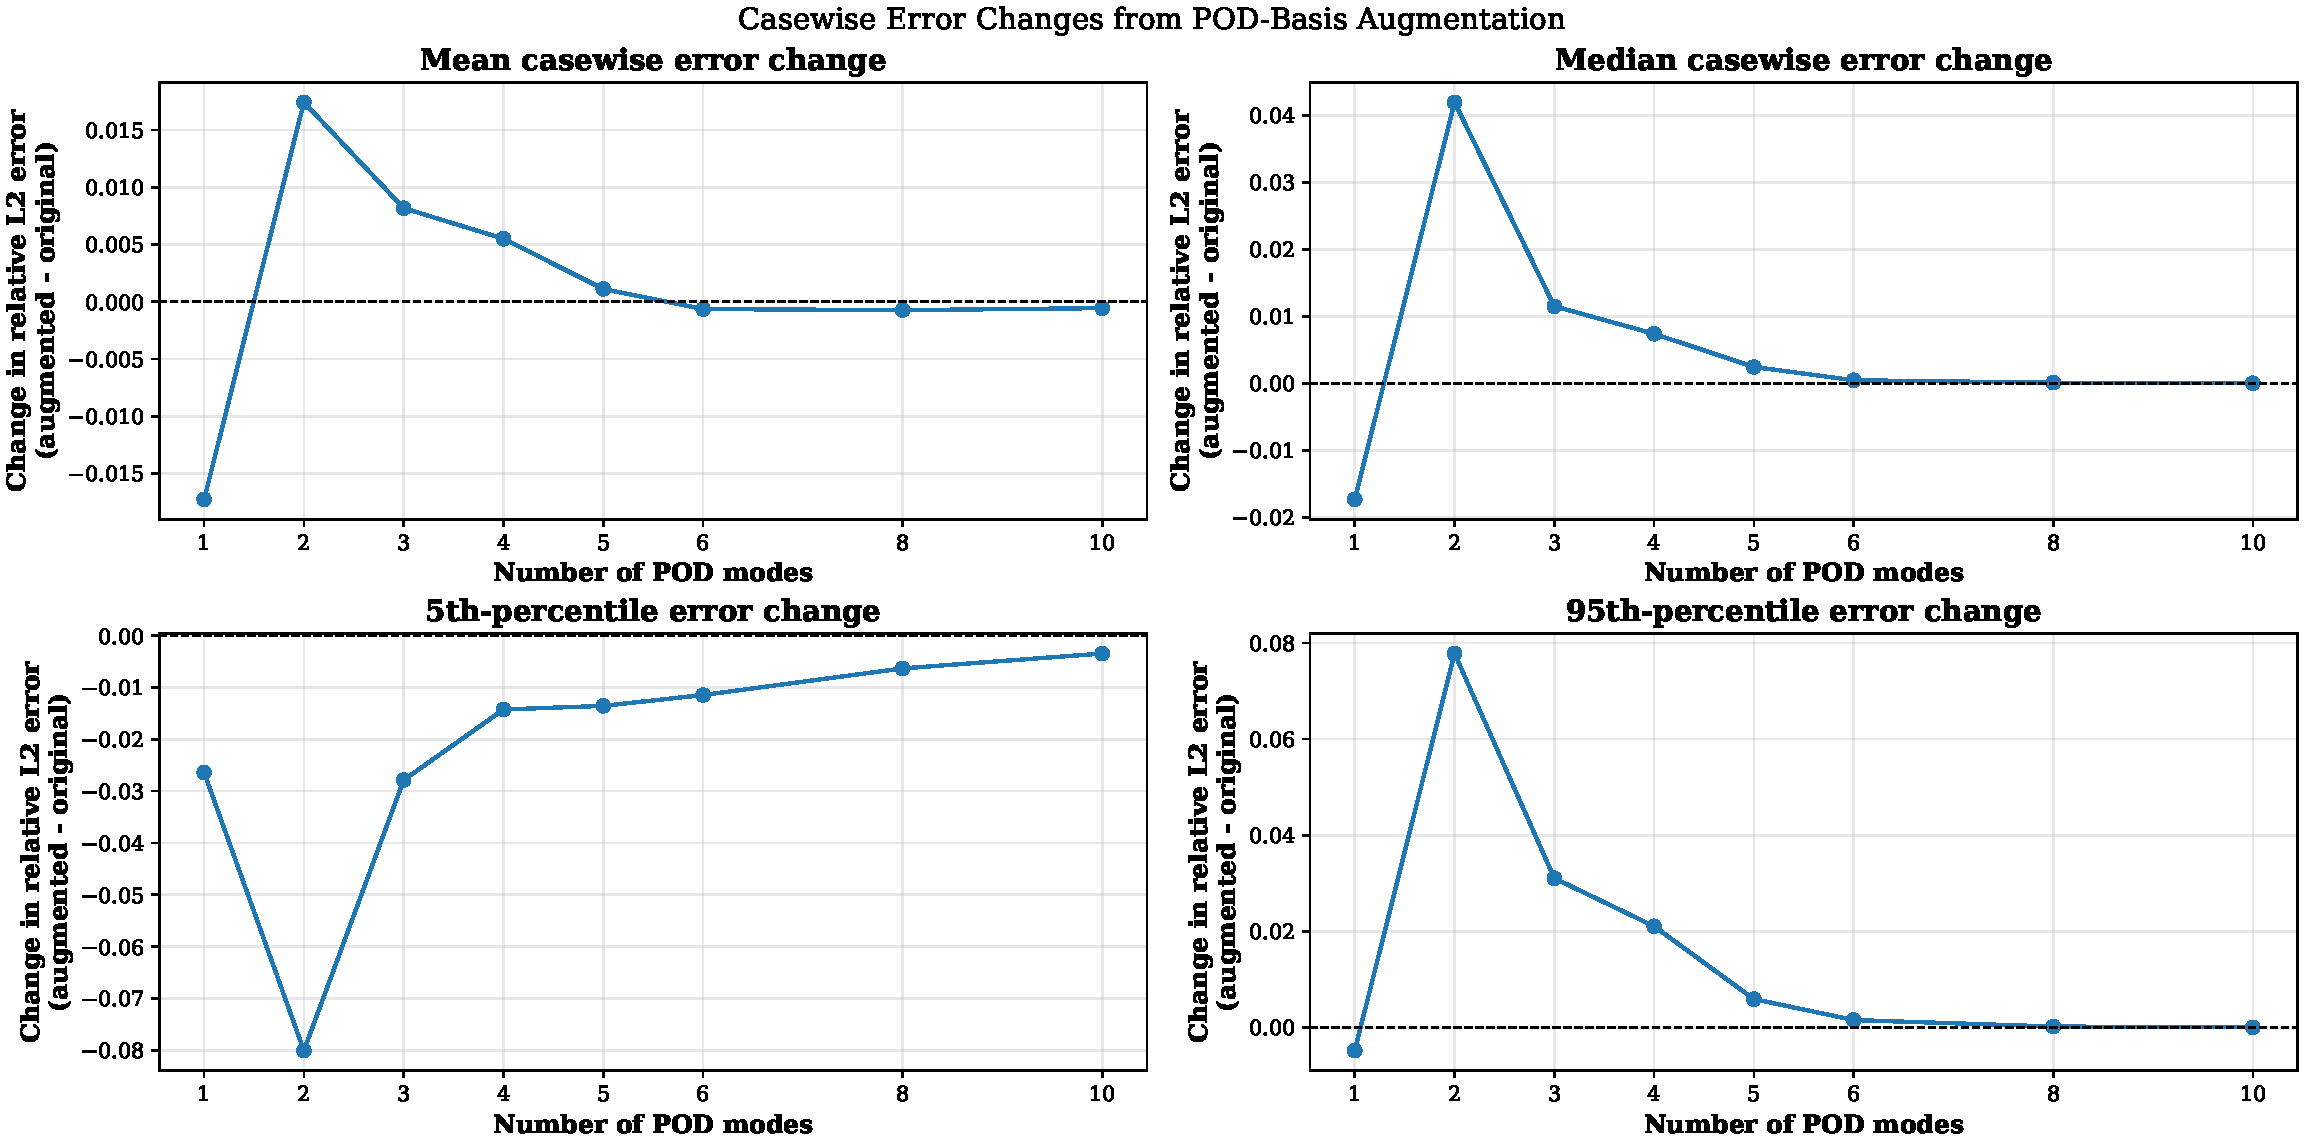
\includegraphics[width=0.95\textwidth]
    {figures/original_augmented_rom_comparison_error_reduction.pdf}
    \caption{Relative error reductions obtained with
    the augmented POD basis compared with the
    original basis for different retained mode counts.}
    \label{fig:original_augmented_error_reduction}
\end{figure}

The parameter-space error maps provide a more
localized comparison. In particular, the ten-mode
comparison is shown in
Figure~\ref{fig:augmented_error_map_ten_modes}.

\begin{figure}[htbp]
    \centering
    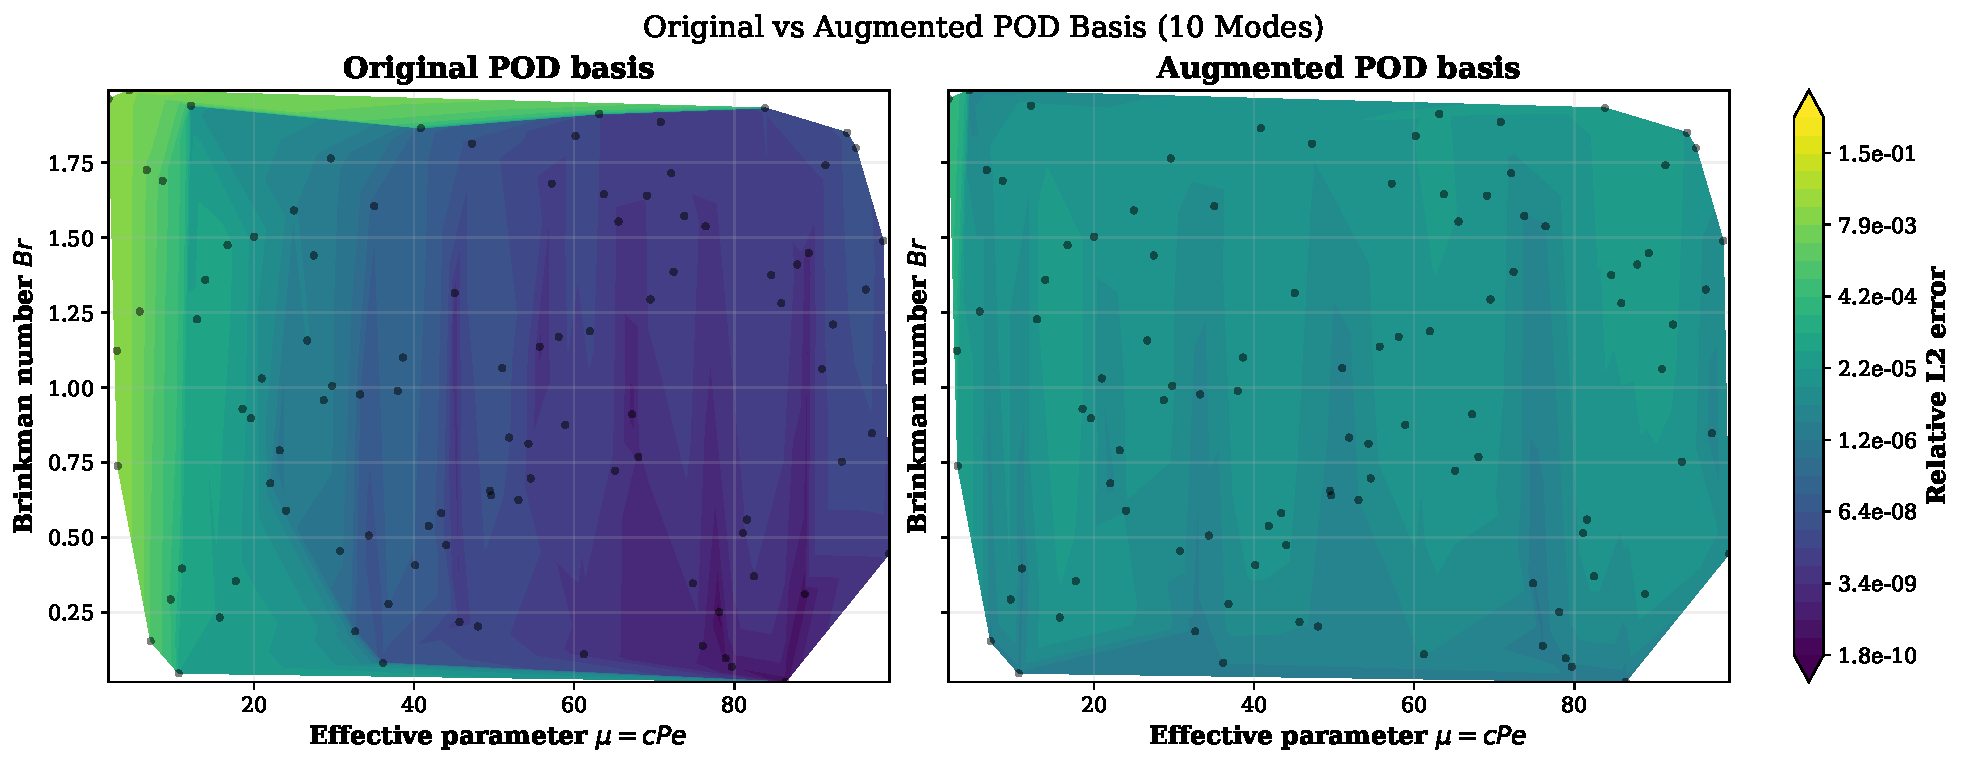
\includegraphics[width=0.95\textwidth]
    {figures/error_map_10_modes.pdf}
    \caption{Triangulated comparison of the original
    and augmented ROM relative $L_2$ errors over
    the independent test parameter domain for
    ten retained modes.}
    \label{fig:augmented_error_map_ten_modes}
\end{figure}

The error maps should be interpreted together with
the paired statistics. They show how the changes
in prediction error are distributed over the
parameter domain, whereas the aggregate statistics
describe their overall magnitude. The reduction
in the largest errors at higher mode counts is
consistent with the purpose of the targeted
enrichment: adding snapshots near parameter regions
where the original basis had difficulty representing
the solution.

\paragraph{Additional error measures and computational time.}

The RMSE and maximum absolute error provide further
information about the temperature-field differences.
For ten modes, the mean RMSE decreases from
$3.786\times10^{-3}$ to $7.24\times10^{-5}$.
The maximum absolute error over all test cases
decreases from 0.434450 to 0.014533.

The mean ROM computation times are also compared.
For the original basis, they range from approximately
$3.07\times10^{-4}$ to
$5.15\times10^{-4}$ seconds per case. For the
augmented basis, they range from approximately
$3.07\times10^{-4}$ to
$7.05\times10^{-4}$ seconds per case. These
measurements indicate a small increase in evaluation
time for most of the higher mode counts. However,
the times remain sub-millisecond, and the differences
should be interpreted with care because of their
small magnitude.

\paragraph{Overall discussion.}

The snapshot-enrichment procedure successfully
increased the training dataset from 100 to 115
full-order snapshots, with all additional simulations
converging. The independent paired evaluation shows
that the resulting augmented basis does not improve
the ROM uniformly across the parameter domain.

At low and intermediate mode counts, the augmented
basis generally produces higher mean errors, although
the maximum errors decrease at four and five modes.
At six, eight, and ten modes, both the mean and
maximum errors decrease substantially. The
ten-mode results are particularly pronounced, with
approximately 97\% reductions in both quantities.

However, the percentage of improved individual
test cases remains low at these higher mode counts.
In particular, only 20\% of the cases improve at
ten modes. This indicates that the enrichment
strongly improves a limited set of parameter
combinations, while it slightly degrades the
approximation for many others.

The results therefore suggest that local snapshot
enrichment is effective at reducing the large
errors associated with selected regions of the
parameter domain, but does not necessarily improve
the global approximation uniformly. The augmented
basis changes the distribution of spatial modes,
and the effect of this change depends on the
retained basis dimension and the parameter
combination being evaluated.

For the present enrichment strategy, the main
benefit is a substantial reduction in the upper
end of the error distribution at higher mode
counts, rather than a consistent improvement for
every test case. Further refinement would therefore
need to consider both the high-error regions and
the broader parameter-space accuracy when selecting
additional snapshots.


\subsection{Computational cost}
\label{subsec:computational_cost}

The Galerkin--POD formulation reduces the dimension of
the governing system from the original full-order spatial
dimension to the number of retained POD modes. For the
present computational grid, the full-order temperature
field contains
\[
N=N_xN_y=50\times20=1000
\]
physical degrees of freedom. In the three-mode
configuration considered here, the reduced system
contains only three unknown modal coefficients:
\[
\mathbf{A}_r\mathbf{a}=\mathbf{b}_r,
\qquad
\mathbf{a}\in\mathbb{R}^{3}.
\]
Thus, the reduced linear system has only three unknowns,
compared with the 1000 unknowns of the full-order
spatial problem. This corresponds to a 99.7\% reduction
in the number of system unknowns.

After solving the reduced system, the complete
temperature field is reconstructed through
\[
\boxed{
\mathbf{T}_{\mathrm{ROM}}
=
\mathbf{T}_{\mathrm{ref}}+\mathbf{V}_3\mathbf{a}.
}
\]
Although the reduced solve involves only three
coefficients, the reconstruction still produces
a temperature vector with 1000 physical values.

\paragraph{Full-order and reduced-order computation times.}

The recorded computation times for the 100 full-order
training cases and the corresponding reduced-order
evaluations are summarized in
Table~\ref{tab:computational_time_comparison}.
The ROM calculations use three retained POD modes.

\begin{table}[htbp]
    \centering
    \caption{Recorded full-order and reduced-order
    computation times for the three-mode ROM.}
    \label{tab:computational_time_comparison}
    \begin{tabular}{lccccc}
        \toprule
        \textbf{Model} &
        \textbf{Cases} &
        \textbf{Mean (s)} &
        \textbf{Median (s)} &
        \textbf{Minimum (s)} &
        \textbf{Maximum (s)} \\
        \midrule
        FOM & 100 & 0.137740 & 0.136677 & 0.099995 & 0.218700 \\
        ROM & 99  & 0.054623 & 0.050581 & 0.046414 & 0.122380 \\
        \bottomrule
    \end{tabular}
\end{table}

The mean recorded full-order computation time is
approximately 0.138~s per case. The mean of the
99 supplied ROM timing records is approximately
0.0546~s. The corresponding median times are
approximately 0.1367~s and 0.0506~s, respectively.

The timing records therefore indicate that the
reduced-order calculations require less computation
time per case than the full-order simulations.
However, one ROM timing entry is missing from the
provided dataset. Consequently, the two reported
means are based on different numbers of records,
and a definitive paired speedup ratio is not
reported here.

\paragraph{Operator construction and reduced-system evaluation.}

The total computational cost of the ROM can be
separated into operator construction, Galerkin
projection, reduced-system solution, and temperature
reconstruction:
\[
\begin{aligned}
t_{\mathrm{ROM}}
={}&t_{\mathrm{operators}}
+t_{\mathrm{projection}}\\
&+t_{\mathrm{reduced\ solve}}
+t_{\mathrm{reconstruction}}.
\end{aligned}
\]

The operator-construction stage includes the assembly
of the full-order convection and diffusion matrices,
the viscous-dissipation source, and the lifting
contribution. These quantities are then projected
onto the retained POD basis.

The reduced-system evaluation stage consists of
assembling the parameter-dependent reduced matrix
and right-hand-side vector, solving the resulting
$3\times3$ linear system, and reconstructing the
temperature field.

For a fixed computational grid and prescribed
velocity field, the full-order spatial operators
and viscous-dissipation source are independent of
the parameter values. Their reduced projections
can therefore be constructed once and reused for
multiple parameter combinations. This would allow
the operator construction and projection costs to
be treated as an offline computational stage,
while the reduced-system solution and reconstruction
would form the online stage.

However, the current implementation reconstructs
the full-order operator components for individual
parameter cases before performing the reduced
projection and solution. Therefore, the current
workflow does not yet fully exploit the potential
offline-online separation.

The timing summary provided here contains the
overall FOM and ROM computation times, but does
not provide the numerical breakdown of operator
construction, projection, reduced-system solution,
and reconstruction. These contributions should
be reported separately using their respective
timing records. In particular, the reduced linear
solve time alone should not be interpreted as the
complete ROM evaluation time.

A consistent comparison of computational
efficiency should include all operations required
to produce the reconstructed ROM temperature
field and compare them with the complete
full-order solution process. Any one-time
preprocessing cost should be reported separately
from the per-parameter evaluation cost.

\subsection{Limitations}
\label{subsec:limitations}

The present reduced-order model has several limitations.
First, the velocity field is prescribed and remains fixed;
therefore, the model does not account for changes in the
flow field or flow-temperature coupling. The parameter
study is restricted to $\mu$ and $Br$, with $c=1$.
Furthermore, all simulations use a fixed $50\times20$
computational grid, and the final ROM represents only
steady-state solutions.

The snapshot-enrichment strategy also depends on the
high-error regions identified in the initial LHS
screening dataset. Consequently, the selected hotspots
reflect the behavior of the original ROM over that
particular sample. The augmented basis does not improve
the accuracy uniformly: its effect depends on the
retained mode count and parameter combination.

Although the final 100-case test dataset excludes
parameter combinations used in the original and
augmented training datasets, its complete independence
from the initial screening dataset should also be
confirmed. Since the screening results were used to
select the enrichment locations, any overlap with the
final test set could affect the interpretation of the
comparison. Therefore, claims about generalization
should be limited to the evaluated parameter domain
and supported by a check for overlap with both the
training and screening datasets.


\section{Conclusions and Future Work}
\label{sec:conclusions}

\subsection{Conclusions}

A discrete Galerkin--POD reduced-order model was developed
for the parameterized steady-state energy equation. The
full-order model was used to generate temperature
snapshots, from which an original POD basis was
constructed. The discretized governing equation was
then projected onto the retained modes to obtain a
reduced system for calculating the modal coefficients.

The original basis was assessed using 100 independent
LHS samples and different retained mode counts.
Increasing the number of modes substantially reduced
the prediction errors. The mean relative $L_2$ error
decreased from 39.56\% with one mode to 0.0468\%
with ten modes.

An adaptive snapshot-enrichment procedure was
subsequently developed. Three high-error parameter
regions were selected, and 15 additional full-order
snapshots were generated around them. These snapshots
were combined with the original 100 snapshots to
construct an augmented POD basis.

The final comparison used 100 test cases excluded
from both POD training datasets. The results showed
that enrichment did not improve the ROM uniformly.
At two to five modes, the mean relative error
increased. At six, eight, and ten modes, it decreased
by 40.77\%, 83.91\%, and 96.98\%, respectively.
At ten modes, the maximum relative error also
decreased by 96.92\%. However, only 20\% of the
individual test cases improved at this mode count.

These findings indicate that targeted snapshot
enrichment can substantially reduce large prediction
errors at higher basis dimensions, but may degrade
accuracy for other parameter combinations. Its
effect therefore depends on both the retained
basis dimension and the location within the
parameter domain.

\subsection{Future Work}

Future work can investigate alternative hotspot
selection criteria and parameter-space sampling
strategies to improve the distribution of prediction
errors. Different enrichment rules and mode-dependent
basis construction could also be examined to obtain
more consistent improvements across test cases.

The evaluation could be extended to larger independent
test datasets to further assess generalization.
Finally, precomputing and storing reusable reduced
operators would improve the offline-online structure
of the implementation and provide a more complete
assessment of its computational efficiency.


%================================================
% Appendices
%================================================

\clearpage

\appendix

\appendix

\section{Supplementary ROM Error Maps}
\label{app:supplementary_error_maps}

This appendix presents the triangulated parameter-space
error maps obtained from the paired comparison of the
original and augmented POD bases. The maps complement
the aggregate statistics discussed in
Section~\ref{subsec:original_augmented_comparison} by
showing the spatial distribution of the relative
$L_2$ errors over the independent test parameter set.

Each map compares the original and augmented ROM
errors for a fixed number of retained POD modes.
The eight mode counts considered are
$r\in\{1,2,3,4,5,6,8,10\}$.

The triangulation-based representation is used because
the independent LHS test points do not form a structured
rectangular grid. The interpolated contours provide a
visual representation of the sampled errors over the
parameter domain.

\begin{figure}[htbp]
    \centering
    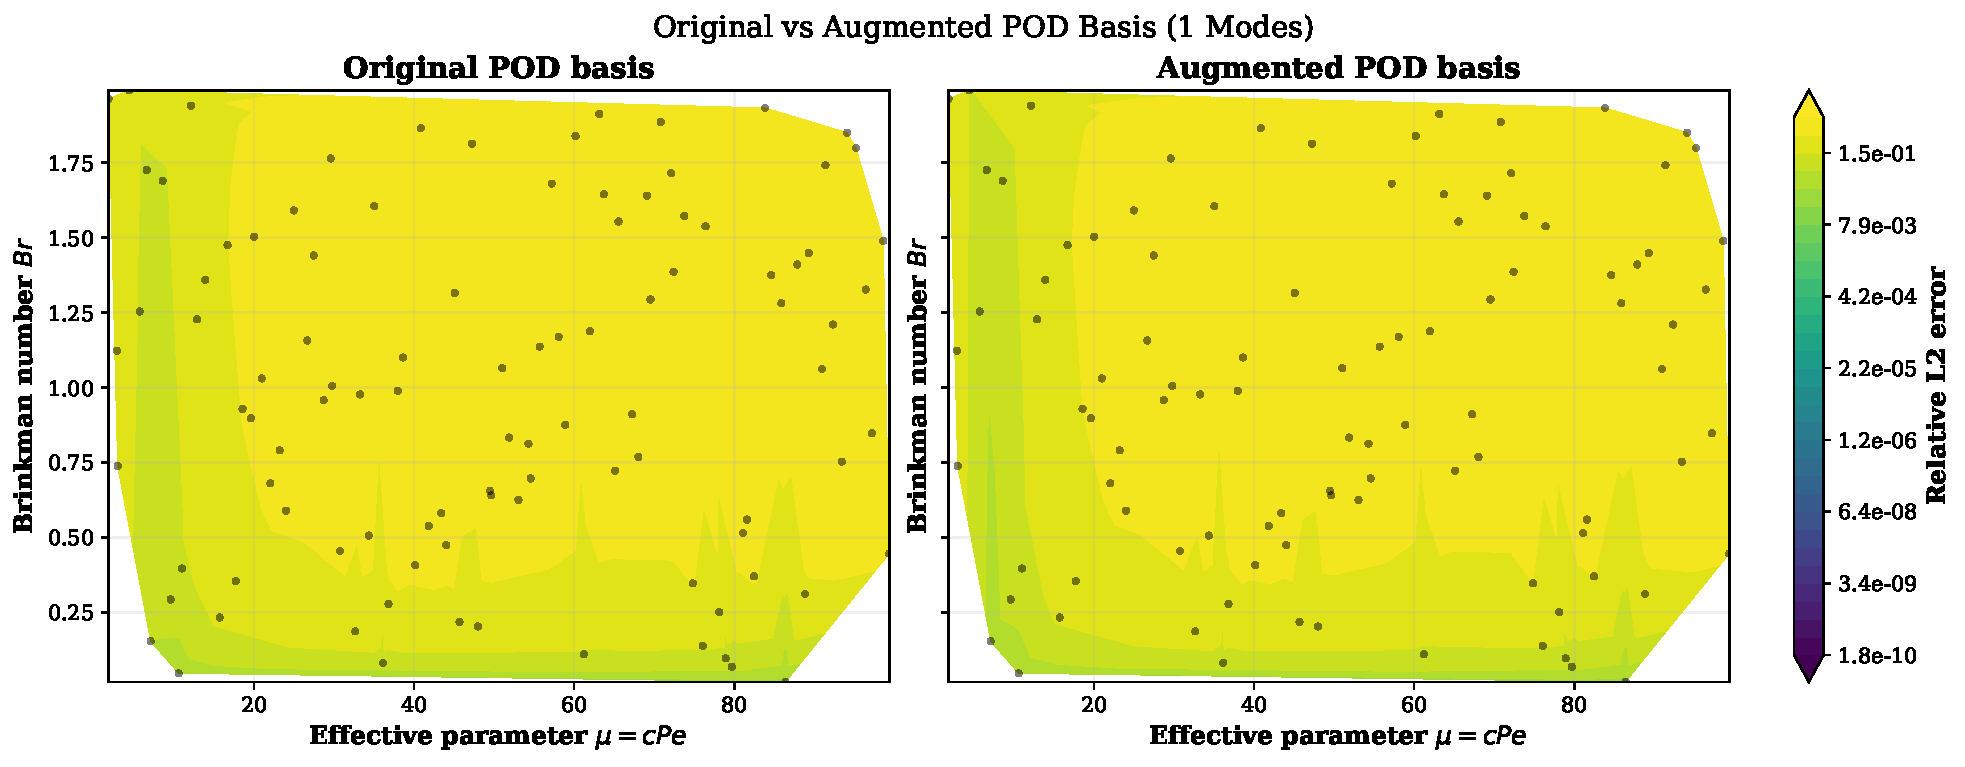
\includegraphics[width=0.95\textwidth]
    {figures/error_map_1_modes.pdf}
    \caption{Original and augmented ROM relative
    $L_2$ error distributions for one retained mode.}
    \label{fig:app_error_map_1}
\end{figure}

\begin{figure}[htbp]
    \centering
    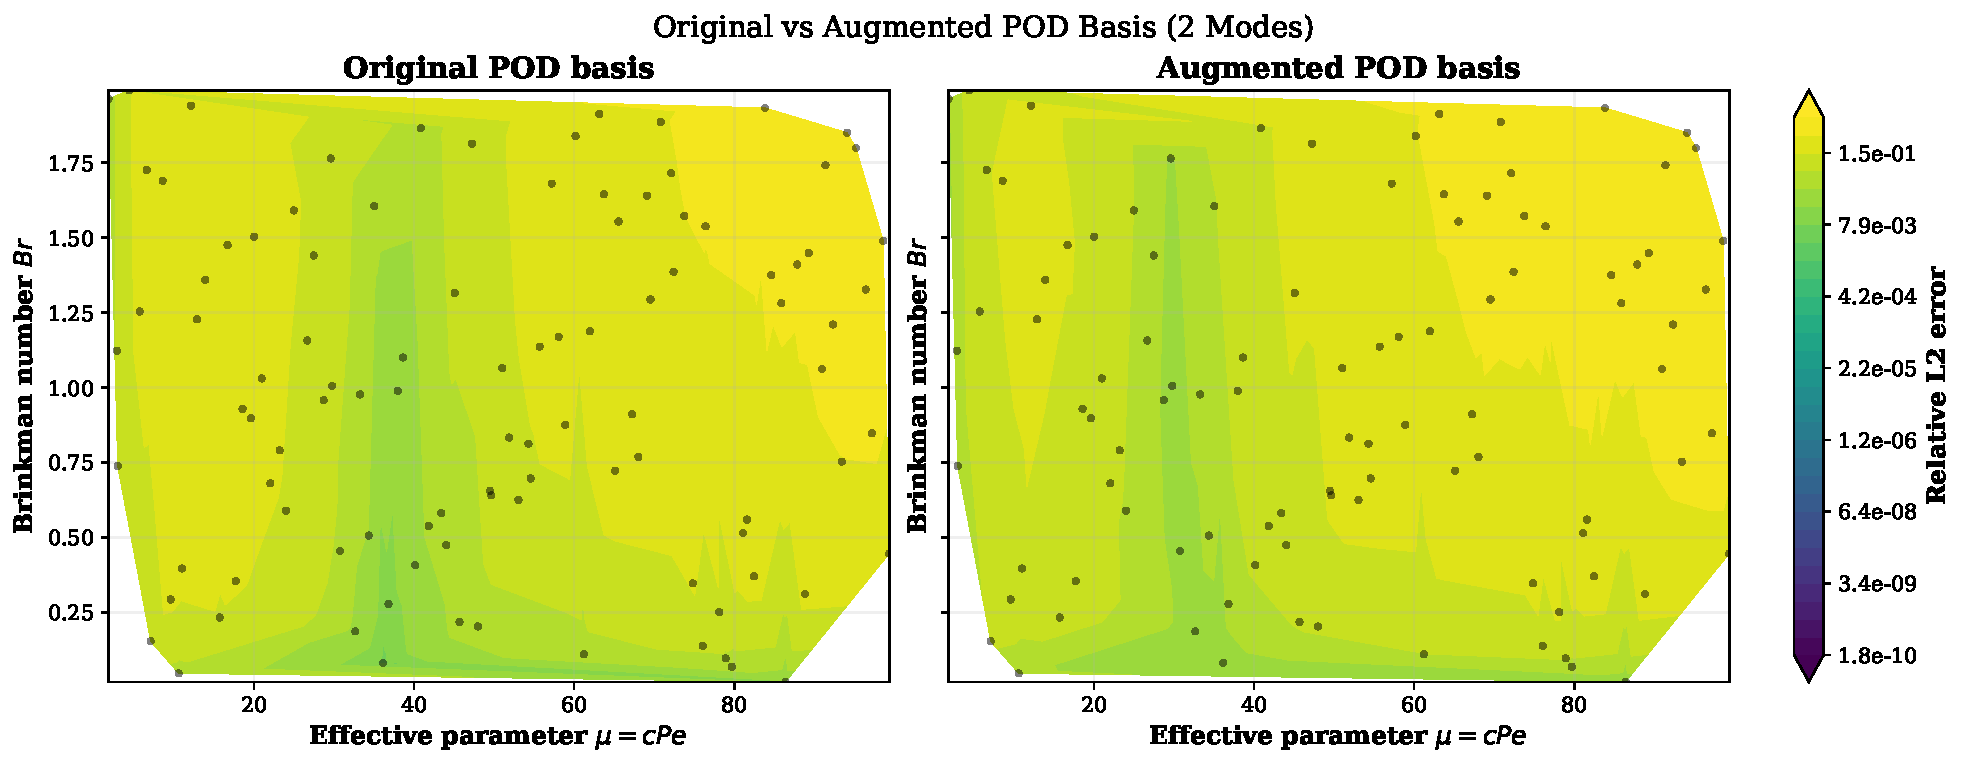
\includegraphics[width=0.95\textwidth]
    {figures/error_map_2_modes.pdf}
    \caption{Original and augmented ROM relative
    $L_2$ error distributions for two retained modes.}
    \label{fig:app_error_map_2}
\end{figure}

\begin{figure}[htbp]
    \centering
    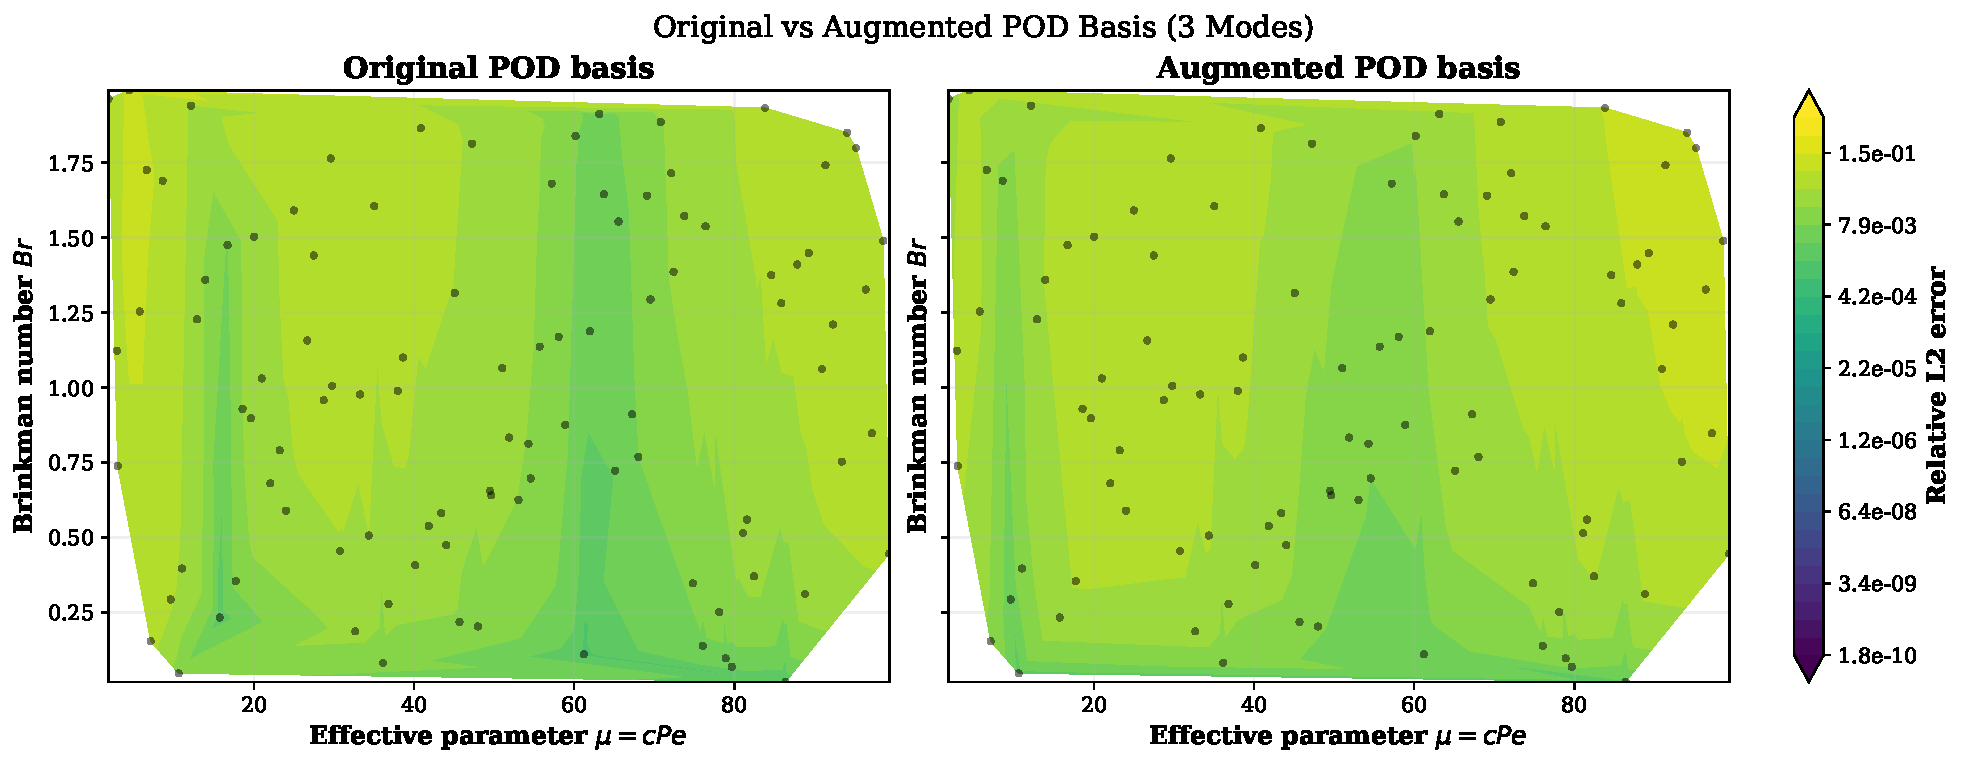
\includegraphics[width=0.95\textwidth]
    {figures/error_map_3_modes.pdf}
    \caption{Original and augmented ROM relative
    $L_2$ error distributions for three retained modes.}
    \label{fig:app_error_map_3}
\end{figure}

\begin{figure}[htbp]
    \centering
    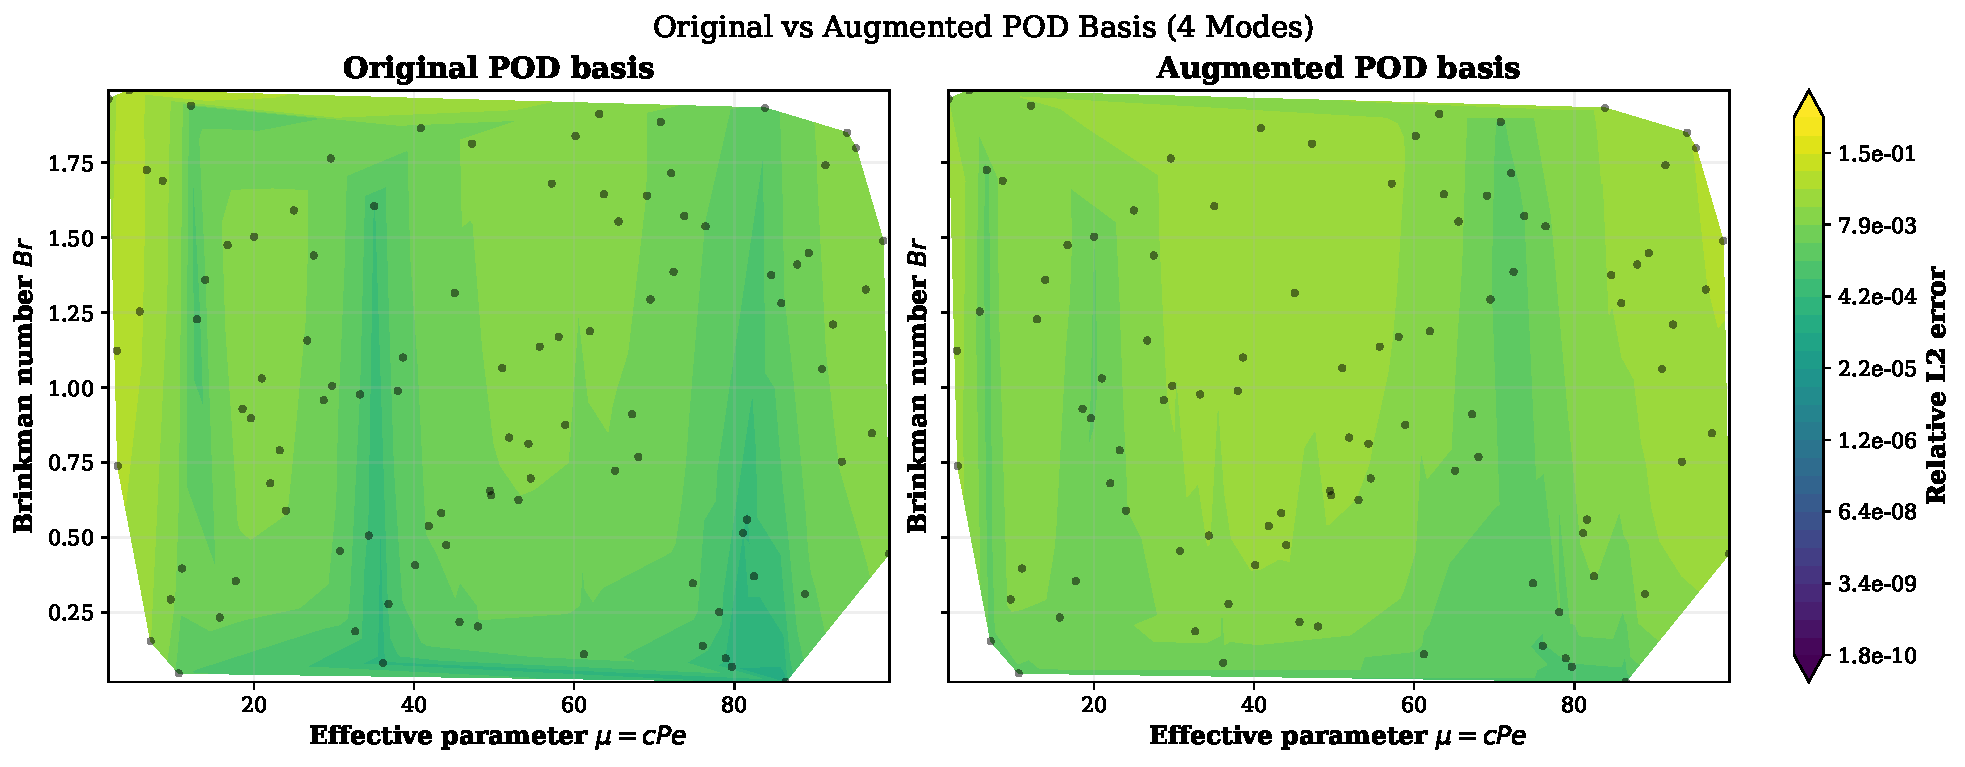
\includegraphics[width=0.95\textwidth]
    {figures/error_map_4_modes.pdf}
    \caption{Original and augmented ROM relative
    $L_2$ error distributions for four retained modes.}
    \label{fig:app_error_map_4}
\end{figure}

\begin{figure}[htbp]
    \centering
    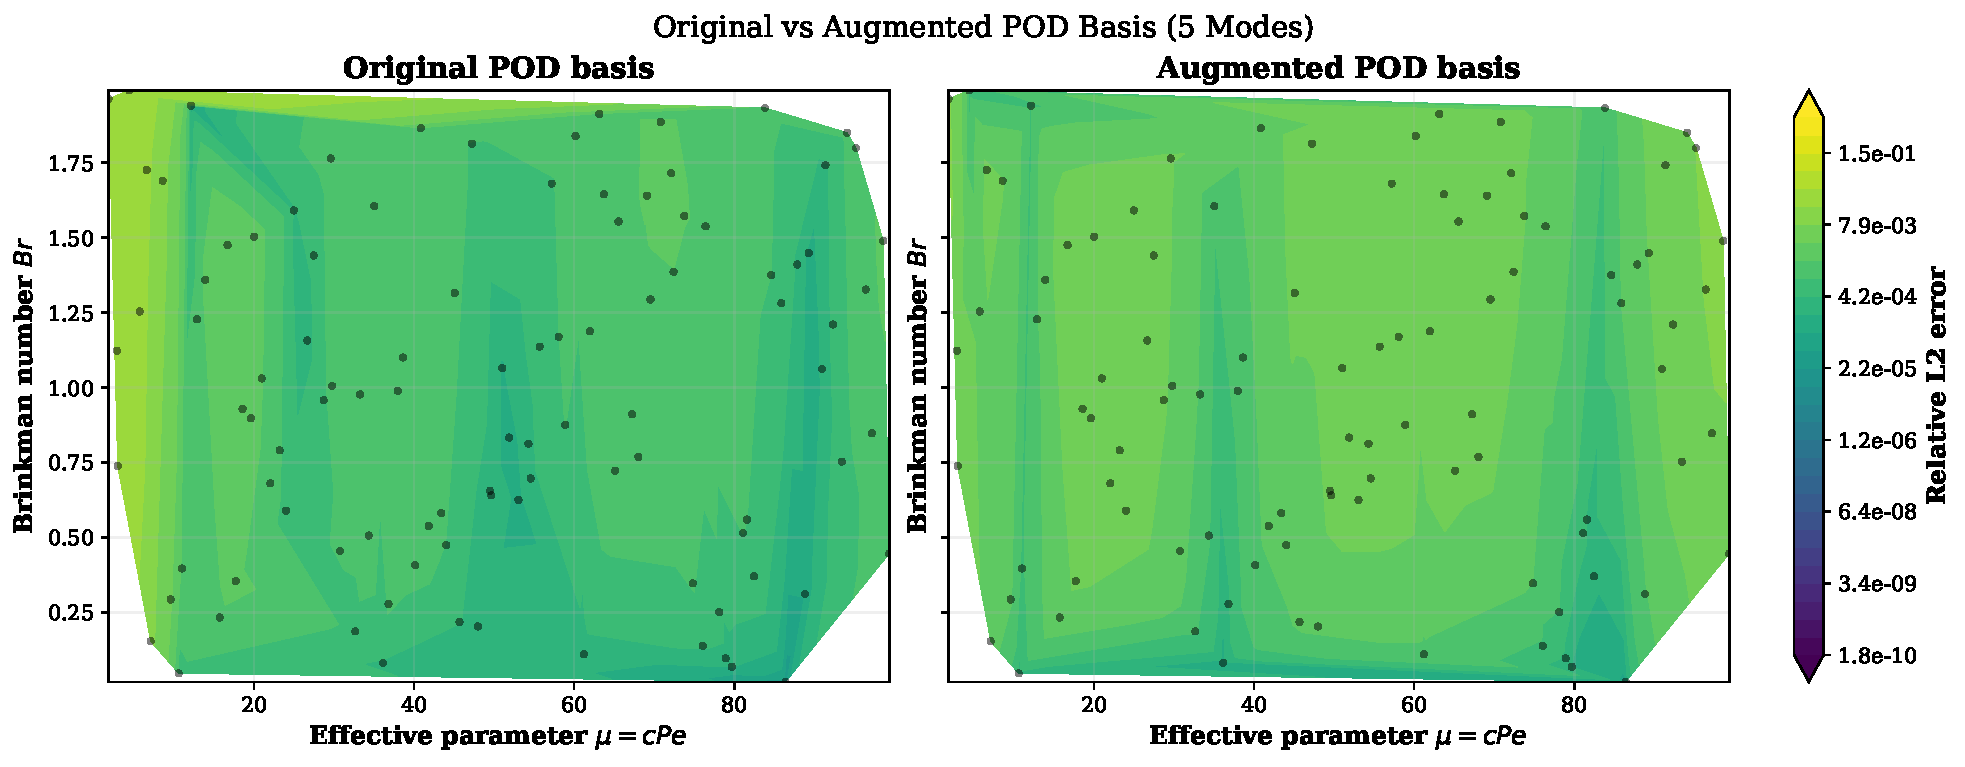
\includegraphics[width=0.95\textwidth]
    {figures/error_map_5_modes.pdf}
    \caption{Original and augmented ROM relative
    $L_2$ error distributions for five retained modes.}
    \label{fig:app_error_map_5}
\end{figure}

\begin{figure}[htbp]
    \centering
    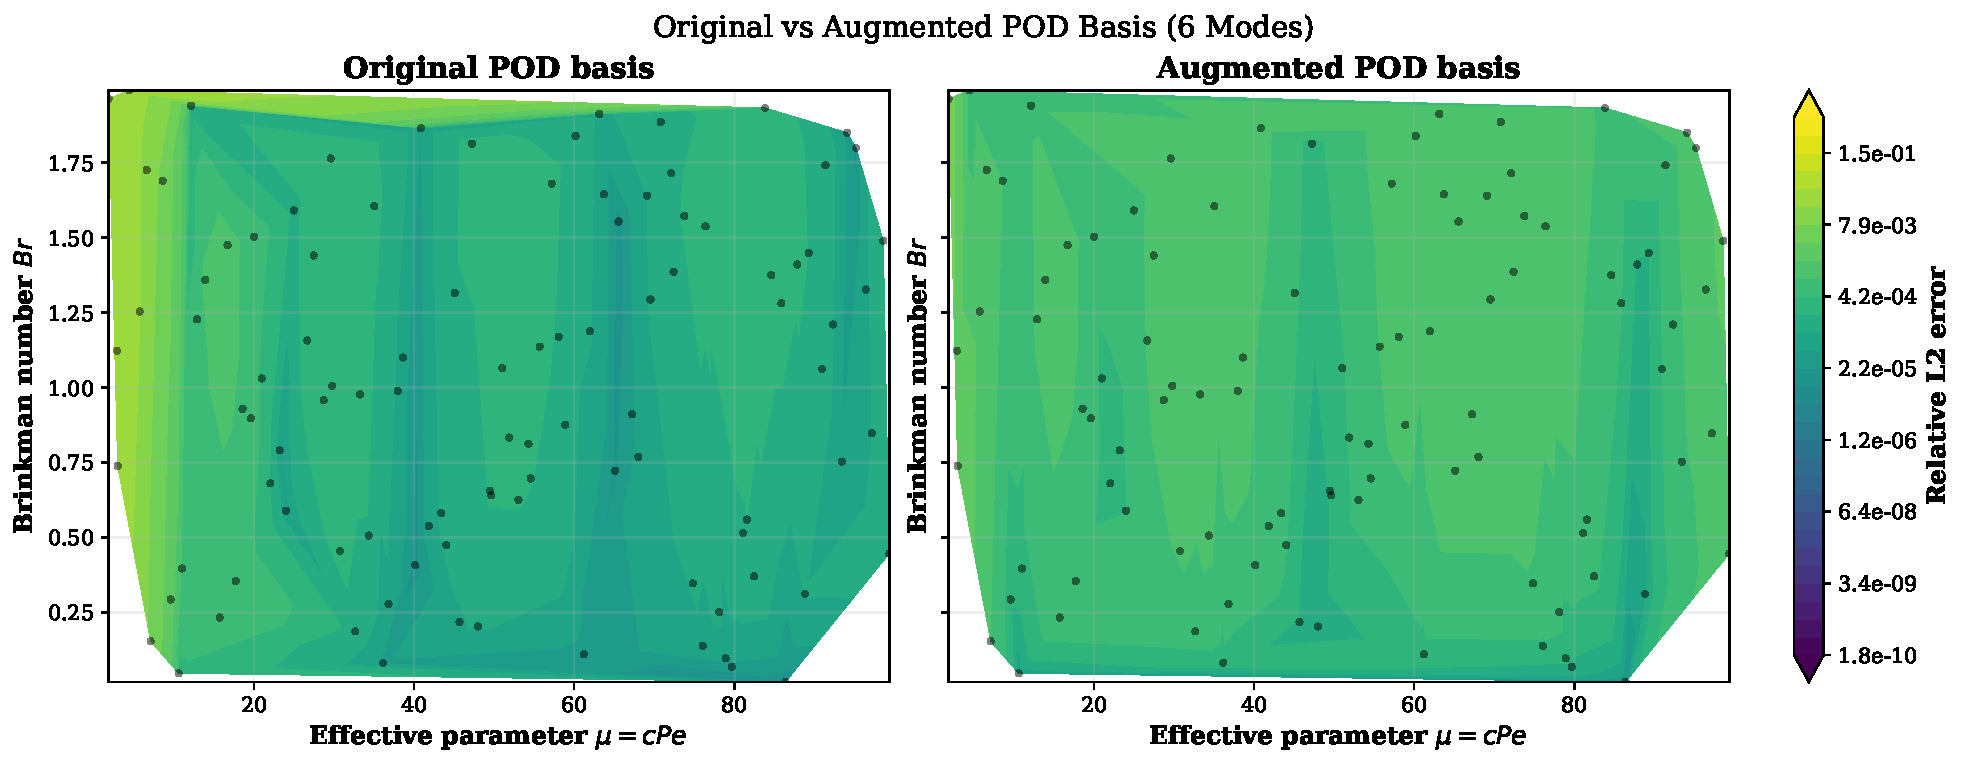
\includegraphics[width=0.95\textwidth]
    {figures/error_map_6_modes.pdf}
    \caption{Original and augmented ROM relative
    $L_2$ error distributions for six retained modes.}
    \label{fig:app_error_map_6}
\end{figure}

\begin{figure}[htbp]
    \centering
    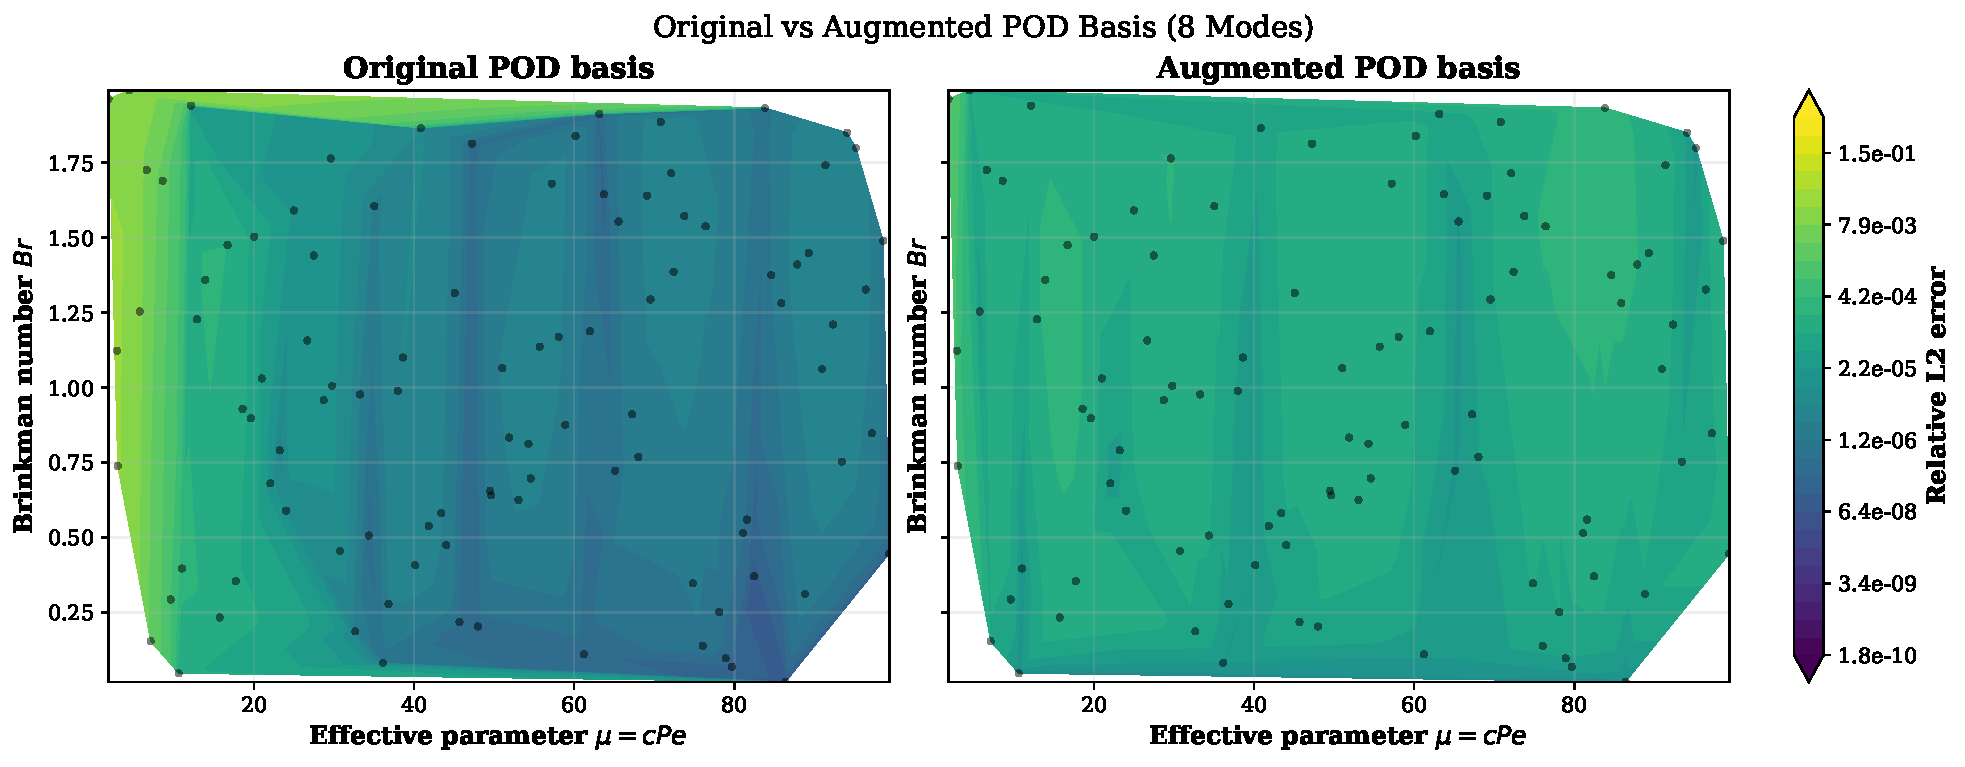
\includegraphics[width=0.95\textwidth]
    {figures/error_map_8_modes.pdf}
    \caption{Original and augmented ROM relative
    $L_2$ error distributions for eight retained modes.}
    \label{fig:app_error_map_8}
\end{figure}

\begin{figure}[htbp]
    \centering
    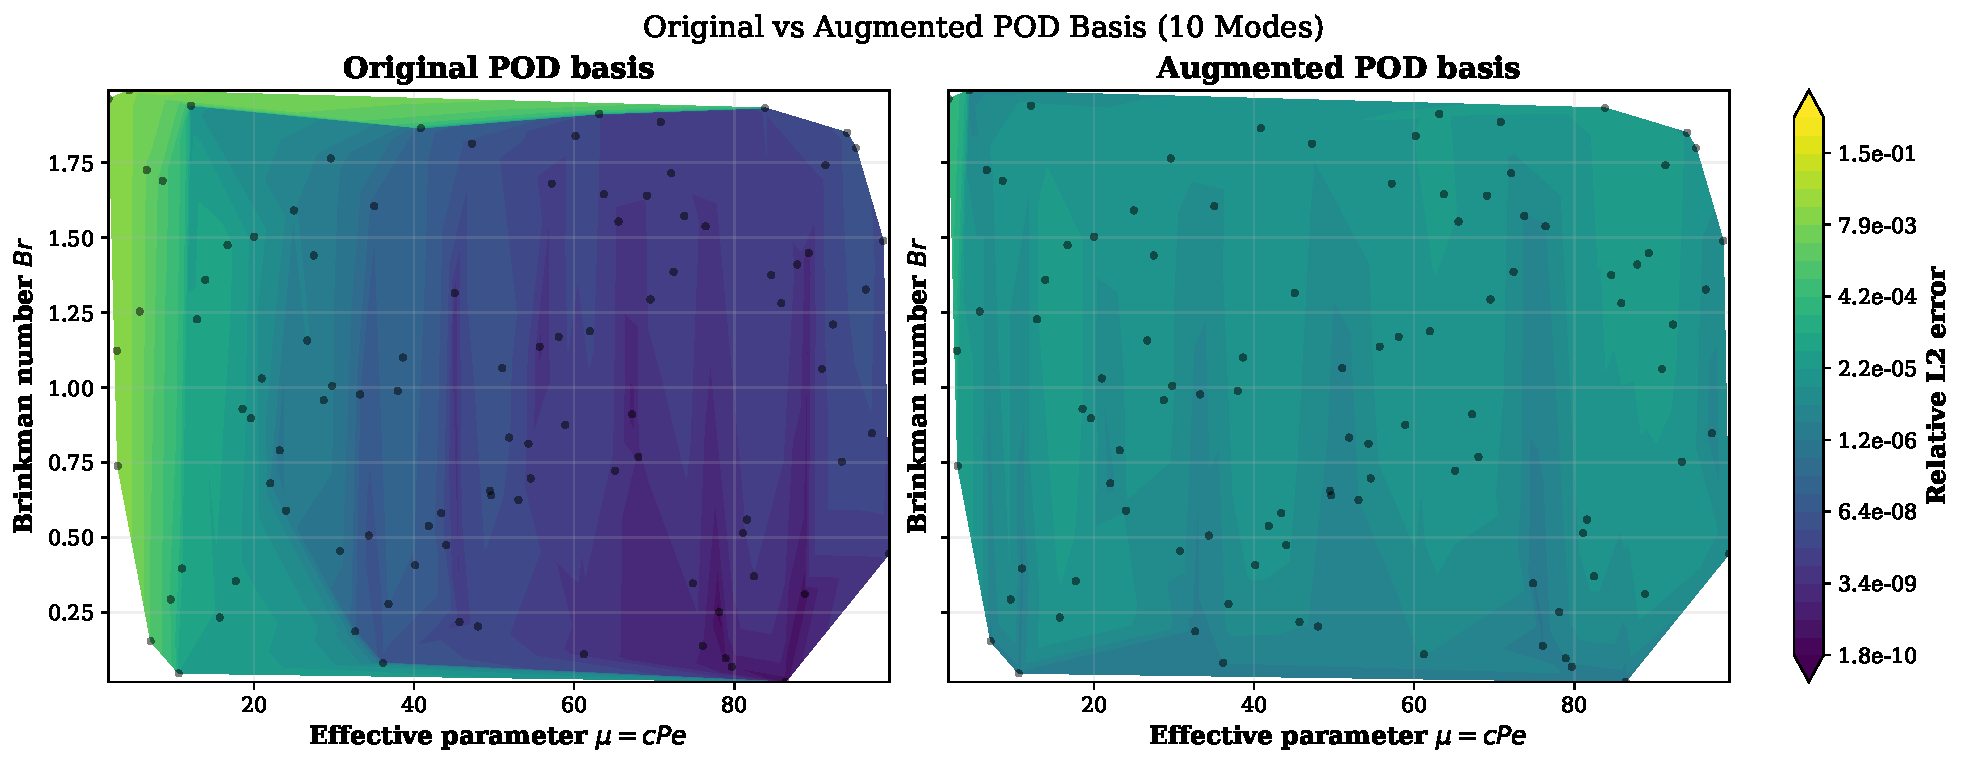
\includegraphics[width=0.95\textwidth]
    {figures/error_map_10_modes.pdf}
    \caption{Original and augmented ROM relative
    $L_2$ error distributions for ten retained modes.}
    \label{fig:app_error_map_10}
\end{figure}


\clearpage

\section{Software Architecture and Implementation Details}
\label{app:software_architecture}

The project is organized into two main directories:
\texttt{src}, which contains the shared numerical
components, and \texttt{Studies}, which contains the
scripts for snapshot generation, POD construction,
Galerkin projection, refinement, and evaluation.

\subsection{Shared numerical modules}

The main source modules are responsible for the
computational grid, initialization, boundary conditions,
diagnostics, and full-order solution.

\paragraph{\texttt{src/grid.py} and
\texttt{src/initialization.py}.}

The function \texttt{create\_grid} generates the
structured grid coordinates. The initialization
module provides the initial temperature field through
\texttt{initialize\_temperature}, which initializes
$T(y)=y$, and constructs the prescribed velocity
components using \texttt{initialize\_velocity\_fields}.

\paragraph{\texttt{src/boundary\_conditions.py}.}

The function \texttt{apply\_temperature\_boundary\_conditions}
implements the four temperature boundary conditions
using ghost cells. It applies the prescribed inlet
and wall temperatures and the zero-gradient outlet
condition.

\paragraph{\texttt{src/diagnostics.py}.}

The function \texttt{build\_rhs} evaluates the
non-temporal terms of the discretized energy equation.
The function \texttt{steady\_state\_residual\_rms}
calculates the RMS residual over the computational
domain. This residual is used to determine convergence
of the full-order solver.

\paragraph{\texttt{src/solvers/direct.py}.}

The full-order solver is implemented through four
main functions:
\begin{itemize}
    \item \texttt{build\_spatial\_matrix}: Constructs
    the sparse five-diagonal spatial matrix. It maps
    physical two-dimensional indices to the
    one-dimensional system and incorporates
    ghost-cell contributions into the matrix
    coefficients.

    \item \texttt{build\_rhs}: Constructs the
    right-hand-side contribution for an individual
    row.

    \item \texttt{build\_forcing\_field}: Applies
    \texttt{build\_rhs} over the computational domain
    to assemble the forcing vector.

    \item \texttt{solve\_with\_direct}: Assembles
    the spatial matrix and forcing vector, factorizes
    $(\mathbf{I}-\Delta t\mathbf{A})$, advances the
    temperature field, and checks convergence using
    the steady-state RMS residual.
\end{itemize}

\subsection{POD construction and Galerkin implementation}

\paragraph{Original snapshot generation and POD basis.}

The script
\texttt{F05\_refinement/f00\_generate\_large\_training\_cases.py}
generates the 100-case training parameter grid. Its
function \texttt{build\_parameter\_grid} creates the
parameter combinations. Each case is then solved
using \texttt{run\_fom\_case}. Converged temperature
fields are converted into snapshot columns, and
their associated simulation information is stored
in \texttt{snapshot\_case\_records}.

The script
\texttt{F05\_refinement/f01\_build\_pod\_basis.py}
loads the snapshot matrix and its case records,
performs the SVD, calculates the POD energy
distribution, and saves the resulting basis.

\paragraph{\texttt{F04\_galerkin\_rom/f01\_operators.py}.}

This module constructs the full-order operator
components required for Galerkin projection.

The function \texttt{\_assemble\_spatial\_matrix}
builds the spatial matrix used to extract the
convection and diffusion operators.

The function \texttt{build\_linear\_operators}
constructs $\mathbf{C}_h$ and $\mathbf{L}_h$.
The function \texttt{build\_viscous\_dissipation\_source}
calculates the parameter-independent source vector
$\boldsymbol{\Phi}_h$ from the prescribed velocity field.

The function \texttt{build\_lifting\_residual}
calculates the discrete lifting contribution, while
\texttt{\_assemble\_forcing\_field} obtains the
affine forcing through the existing full-order
forcing routine.

The function \texttt{verify\_operator\_decomposition}
provides checks for the consistency of the operator
decomposition and lifting-residual formulation.
Finally, \texttt{build\_operator\_components}
collects the resulting matrices and vectors.

\paragraph{\texttt{F04\_galerkin\_rom/f02\_reduced\_operators.py}.}

This module projects the full-order operators onto
the retained POD basis. It constructs the reduced
convection and diffusion matrices and the projected
viscous-dissipation and lifting vectors:
\[
\begin{aligned}
\mathbf{C}_r&=\mathbf{V}_r^T\mathbf{C}_h\mathbf{V}_r,\\
\mathbf{L}_r&=\mathbf{V}_r^T\mathbf{L}_h\mathbf{V}_r,\\
\boldsymbol{\Phi}_r&=\mathbf{V}_r^T\boldsymbol{\Phi}_h,\\
\mathbf{g}_r&=\mathbf{V}_r^T\mathbf{g}_{\mathrm{lift}}.
\end{aligned}
\]

\paragraph{\texttt{F04\_galerkin\_rom/f03\_solve\_reduced.py}.}

This module handles reduced-system assembly,
solution, and temperature reconstruction.

The function \texttt{construct\_reduced\_system}
assembles the reduced matrix and forcing vector.
The function \texttt{solve\_reduced\_system}
calculates the modal coefficients and returns
the reduced-system residual. The function
\texttt{reconstruct\_temperature} recovers the
temperature field from the modal coefficients
and reference temperature.

The main function, \texttt{run\_reduced\_model},
coordinates these operations and saves the
reduced system, modal coefficients, and
reconstructed temperature field.

\paragraph{Case-level ROM evaluation.}

The script
\texttt{F04\_galerkin\_rom/f04\_rom\_for\_case.py}
provides case-level full-order and reduced-order
evaluations. Its main function,
\texttt{run\_rom\_for\_case}, processes the
specified cases, computes their error metrics,
saves the reconstructed fields and records,
and identifies the minimum- and maximum-error
cases for visualization.

The functions \texttt{run\_fom\_case} and
\texttt{run\_rom\_case} provide the corresponding
full-order and reduced-order calculations.
The script
\texttt{F04\_galerkin\_rom/f05\_test\_rom.py}
generates parameter cases and passes them to
the case-level evaluation routine.

\subsection{Snapshot enrichment and independent evaluation}

The refinement workflow is implemented through
the scripts in \texttt{F05\_refinement}.

\paragraph{Mode-count study.}

The script
\texttt{f03\_mode\_count\_study.py}
evaluates the original POD basis over the LHS
screening dataset. It constructs the full-order
operators, evaluates the ROM for each selected
mode count, records the error metrics, and
generates the error-statistics plots and
triangulated error maps.

\paragraph{Hotspot selection and additional snapshots.}

The script
\texttt{f04\_generate\_augmented\_training\_set.py}
identifies high-error candidates and selects
spatially diverse hotspot centres.

The function \texttt{build\_hotspot\_candidates}
ranks the high-error cases separately for each
selected mode count, groups repeated parameter
combinations, and calculates their mean rank
scores, support fractions, and base scores.

The function \texttt{select\_hotspots} applies
the spatial-diversity criterion. The function
\texttt{build\_augmented\_parameter\_grid}
generates the local parameter combinations
around the selected centres and removes
invalid, duplicate, and previously sampled
points.

Finally, \texttt{run\_augmented\_training\_set\_generation}
solves the additional full-order cases and
saves their temperature fields and records.

\paragraph{Augmented POD basis.}

The script
\texttt{f05\_build\_augmented\_pod\_basis.py}
combines the original and additional snapshot
matrices through
\texttt{combine\_snapshot\_datasets}. The
combined matrix is then decomposed using SVD
to obtain and save the augmented POD basis.

\paragraph{Independent test generation.}

The script
\texttt{f06\_generate\_independent\_test\_set.py}
generates the final LHS test dataset. The
function \texttt{load\_training\_parameter\_keys}
loads the parameter combinations used in the
original and augmented training datasets.
The function \texttt{generate\_test\_parameter\_grid}
generates unique test combinations and excludes
previously used training points.

The main function,
\texttt{run\_independent\_test\_set\_generation},
runs the full-order solver for the accepted
test cases and saves their temperature fields
and simulation records.

\paragraph{Original-versus-augmented comparison.}

The script
\texttt{f07\_compare\_original\_and\_augmented\_bases.py}
performs the final paired comparison.

The function \texttt{run\_basis\_comparison}
loads the independent test cases and both POD
bases, evaluates them at the selected mode
counts, and generates the comparison results.

The function \texttt{run\_rom\_evaluations}
applies each basis to exactly the same test
cases. The function \texttt{build\_comparison\_summary}
calculates the aggregate error statistics,
while \texttt{build\_paired\_comparison}
matches the original and augmented results
case by case. The function
\texttt{build\_improvement\_summary}
then calculates the error changes and
improvement statistics.

Finally, the plotting functions generate the
aggregate error comparisons, error-reduction
plots, and parameter-space error maps.

\subsection{Overall execution sequence}

The main computational workflow can be summarized
as follows:
\begin{enumerate}
    \item Generate full-order training cases and
    construct the original POD basis.
    \item Build the discrete Galerkin operators
    and evaluate the original ROM.
    \item Generate the LHS screening dataset and
    perform the mode-count study.
    \item Select hotspots and generate additional
    full-order snapshots.
    \item Construct the augmented POD basis.
    \item Generate the independent test dataset.
    \item Evaluate both POD bases on the same test
    cases and calculate the paired error statistics.
\end{enumerate}

This organization separates the shared numerical
components from the individual study stages and
allows the full-order solver, POD routines, and
Galerkin implementation to be reused throughout
the refinement and evaluation workflow.


%================================================
\end{document}
